

\chapter{System devices/components - Models and Manufacturers}
This chapter presents the equipment that will compose the electronics architecture of DORIS. The following equipment are considered in this scope:
\begin{itemize}
  \item Computers and accessories
  \item Network devices
  \item Motor and peripheral components
  \item Motor drivers
  \item Electronic components for printed circuit boards (PCBs)
  \item Cables
  \item Connectors
  \item General tools and utilities
\end{itemize}
For each equipment, this chapter presents:
\begin{itemize}
  \item Selected model and manufacturer.
  \item Main features and considerations.
  \item Datasheet and manual references.
  \item Contact for purchasing.
  \item Alternate models/manufacturers.
\end{itemize}

\section{Computers} \label{DEVICE:PC}
\subsection{1\textsuperscript{st} option: ADLQM67PC-2715QE}
\begin{itemize}
  \item Manufacturer: ADL Embedded Solutions\texttrademark
  \item Description:
  \begin{itemize}
    \item This computer model was chosen as the first option for use in DORIS. It can be used for both control and signal processing PC. Its main bus interface is PCI/104-Express, which makes easier the system expansion using PCI/104-Express compatible modules, such as: CAN controller, Ethernet switch, analog-digital converter, frame-grabber, etc. The processor is a 2\textsuperscript{nd} generator Intel Core i7. The fast processing combined with 8GB RAM and 512GB SSD (Solid-State Drive) guarantees DORIS main software requirements: large data amount real-time processing (video, image, audio), traction and manipulator control, mission control management, navigation and data transmission. The SSD drive is a solution for a storage device with no-moving parts, which is suitable for DORIS operation.
  \end{itemize}
  \item Main features:
  \begin{itemize}
    \item Processor: Intel\textregistered Core\texttrademark i7 Gen2 Quad 2.1GHz - 3GHz
    \item Chipset: Intel\textregistered QM67 PCH with PCI/104 Express v1.0a Form Factor
    \item Memory: Up to 8GB DDR3-1333 DRAM SoDIMM204
    \item Storage interface: 2x SATA 600 Ports with RAID (6000MHz)
    \item Operational system: Ubuntu (version 12.04) kernel 3.2.0 running ROS. See G4 project for more information.
    \item Watchdog Timer
    \item Power supply: 5VDC and 12VDC
    \item Power consumption: 45W (full load)
    \item Approx. dimensions: 115mm x 96mm
  \end{itemize}
  \item Main interfaces:
  \begin{itemize}
    \item 2x 10/100/1000 Mbit Ethernet LAN Port
    \item 2x RS232 COM Ports, 8x USB2.0 Ports
  \end{itemize}
  \item Documentation:
  \begin{itemize}
    \item Website: \href{http://adl-usa.com/products/detail/6/adlqm67pc2715qe}{http://adl-usa.com/products/detail/6/adlqm67pc2715qe}
    \item Datasheet: see website.
    \item Manual: see website.
    \item Sales contact: sales@adl-usa.com; sales@adl-europe.com. For more info, see \href{http://adl-usa.com/contact}{http://adl-usa.com/contact}.
  \end{itemize}
\end{itemize}
ADLQM67PC-2715QE picture can be seen in figure~\ref{FIG:DEVICEPCOPTION1}.
\begin{figure}
  \centering
  % Requires \usepackage{graphicx}
  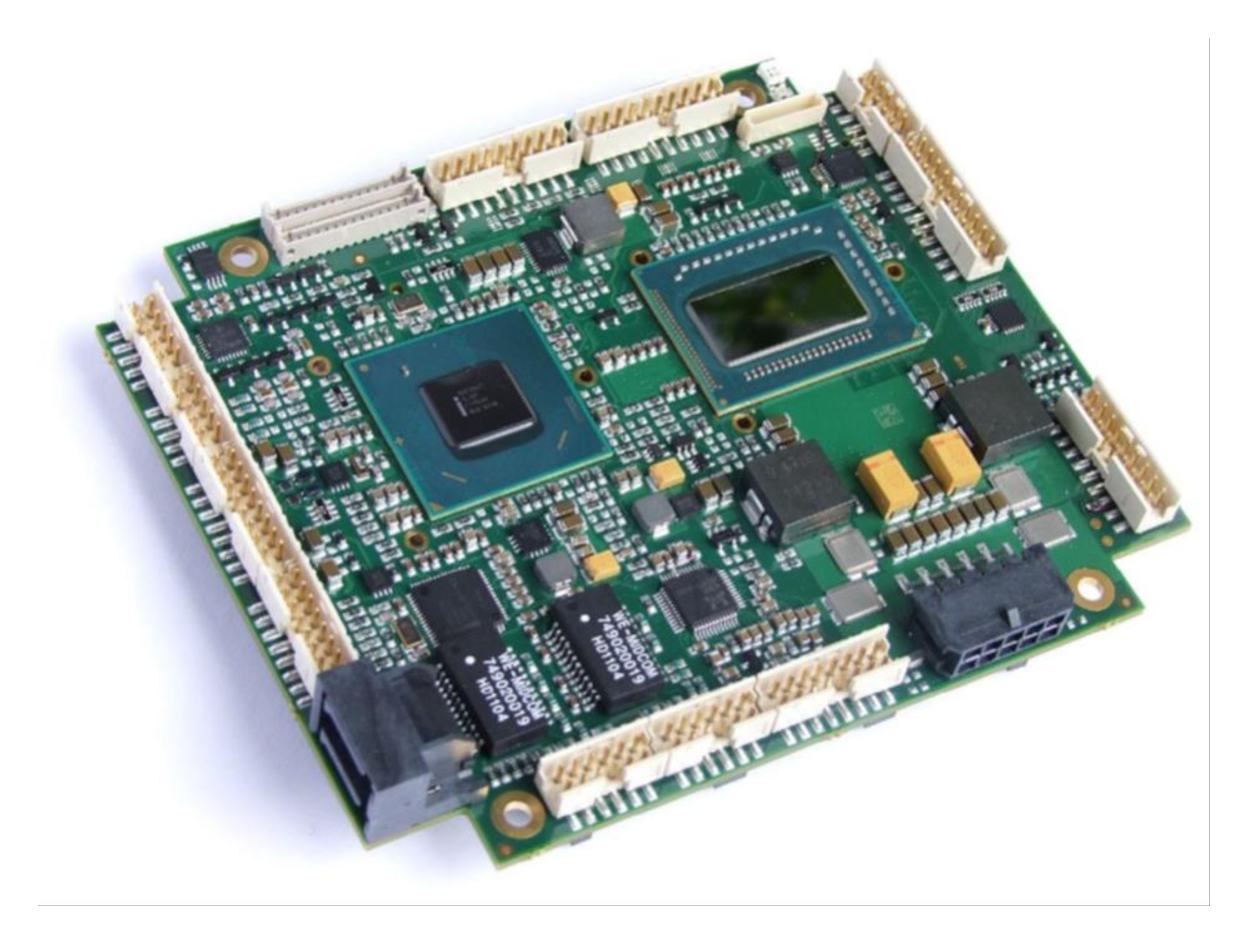
\includegraphics[angle=90,width=1\columnwidth]{figs/body02/FIGDEVICEPCOPTION1.pdf}\\
  \caption[Computer (Option 1): ADLQM67PC-2715QE]{Computer (Option 1): ADLQM67PC-2715QE}
  \label{FIG:DEVICEPCOPTION1}
\end{figure}

\subsection{2\textsuperscript{nd} option: ADLQM87PC}
\begin{itemize}
  \item Manufacturer: ADL Embedded Solutions\texttrademark
  \item Description:
  \begin{itemize}
    \item The preliminary tests involving DORIS PC were performed using the first option (ADLQM67PC-2715QE). But later, this new model was launched onto the market. It was selected as DORIS second PC option, since it is similar to the first option and is superior in some features. Like ADLQM67PC-2715QE, this new model can also be used for both control and signal processing PC.
  \end{itemize}
    \item Enhancements:
  \begin{itemize}
    \item Faster and newer processor, newer chipset, more interface ports (including 5 extra USB ports with different data rates).
  \end{itemize}
  \item Main features:
  \begin{itemize}
    \item Processor: 4\textsuperscript{th} Gen Intel\textregistered Core\texttrademark Dual and Quad Core; BGA1364
    \item Chipset: Intel\textregistered 8-Series PCH Lynx Point QM87 Chipset with PCI/104 Express v1.0a Form Factor
    \item Memory: Up to 8 GB DDR3L-1333/1600; 1.35V SoDIMM204 Socket
    \item Storage interface: 4x SATA 6 Gb/s with RAID 0/1/5/10, Backward Compatible (6000MHz)
    \item Operational system: Ubuntu (version 12.04) kernel 3.2.0 running ROS. See G4 project for more information.
    \item Watchdog Timer
    \item Power supply: 5VDC and 12VDC
    \item Approx. dimensions: 115mm x 96mm
  \end{itemize}
  \item Main interfaces:
  \begin{itemize}
    \item 2x 10/100/1000 Mbit Ethernet LAN Port
    \item 13x USB 2.0. Total:
    \begin{itemize}
      \item 8x Onboard
      \item 2x PCIe Connector
      \item 1x Mini PCIe Socket
      \item 2x USB 3.0
      \item Backward USB 2.0 Compatible
    \end{itemize}
  \end{itemize}
  \item Documentation:
  \begin{itemize}
    \item Website: \href{http://adl-usa.com/products/detail/100/adlqm87pc}{http://adl-usa.com/products/detail/100/adlqm87pc}
    \item Datasheet: see website.
    \item Manual: see website.
    \item Sales contact: sales@adl-usa.com; sales@adl-europe.com. For more info, see \href{http://adl-usa.com/contact}{http://adl-usa.com/contact}.
  \end{itemize}
\end{itemize}
ADLQM87PC picture can be seen in figure~\ref{FIG:DEVICEPCOPTION2}.
\begin{figure}
  \centering
  % Requires \usepackage{graphicx}
  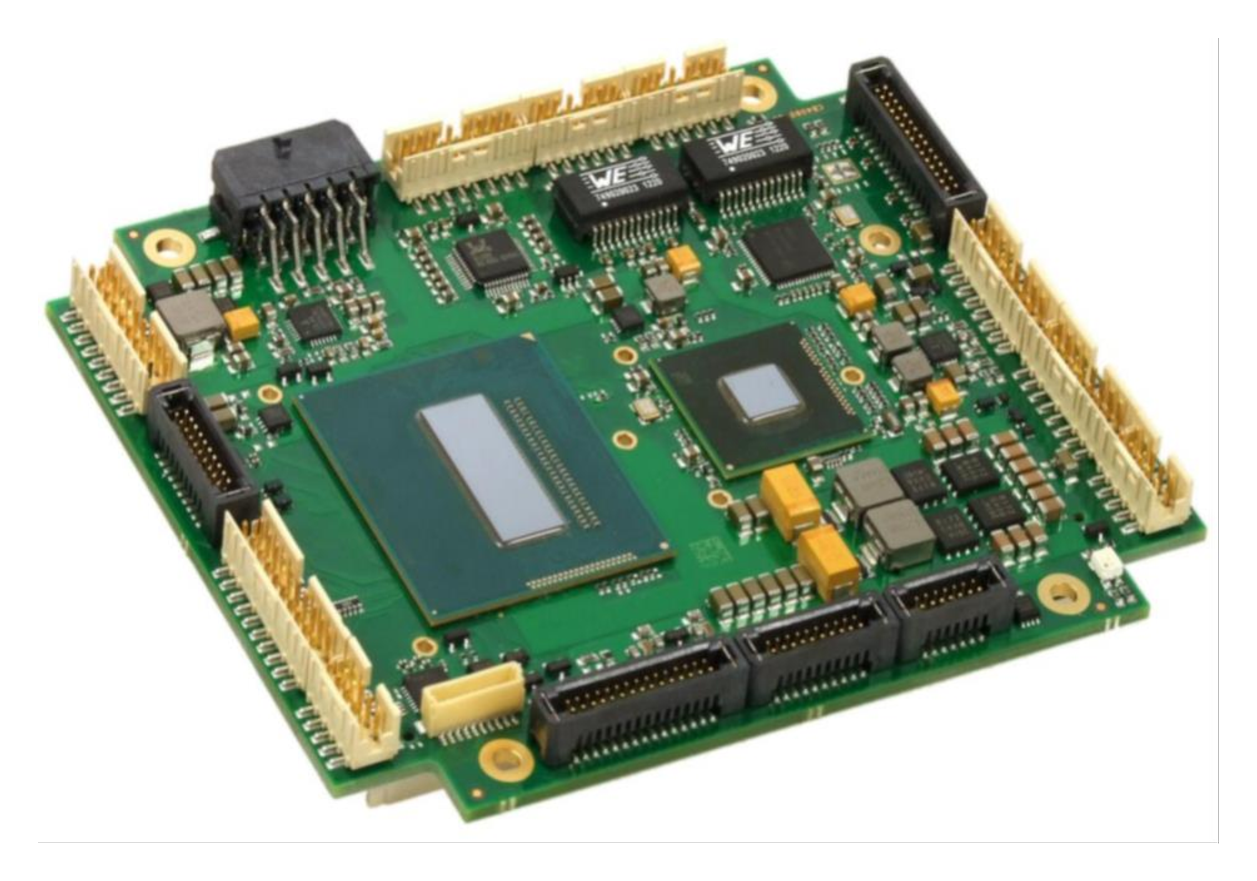
\includegraphics[angle=90,width=1\columnwidth]{figs/body02/FIGDEVICEPCOPTION2.pdf}\\
  \caption[Computer (Option 2): ADLQM87PC]{Computer (Option 2): ADLQM87PC}
  \label{FIG:DEVICEPCOPTION2}
\end{figure}

\subsection{3\textsuperscript{rd} option: Small PC SC240ML-i724 Waterproof Computer}
\begin{itemize}
  \item Manufacturer: Small PC, A Division of ICI Controls, Inc.
  \item Description:
  \begin{itemize}
    \item This PC is a more complete solution for DORIS PC, since it is already designed for reliable operation in hazardous areas and under abnormal situations, which release the user from the need to purchase/fabricate a protection cover. The system is waterproof (IP67), sealed and vibration proof. An specialized heat pipe provides fanless cooling. A SSD drive provides a no-moving parts solution. It is based on a Intel Core i7 processor, with a wide and customizable variety of configurations and I/O options. The system supports optional removal hot swap drives and comes complete with a sealed cable and connectors set.
  \end{itemize}
    \item Superior features:
  \begin{itemize}
    \item Waterproof chassis (IP67), heat-pipe for cooling, sealed cable and connector set, vibration proof, hot swap drives for system expansion.
  \end{itemize}
  \item Main features:
  \begin{itemize}
    \item Processor: Intel\textregistered Core\texttrademark i7 2.4GHz
    \item Chipset: Intel\textregistered NF9G-QM77 Express
    \item Memory: Up to 16GB
    \item Storage interface: Hard Drive capacity up to 1 TB; SSD drive up to 512GB
    \item Operational system: Ubuntu (version 12.04) kernel 3.2.0 running ROS. See G4 project for more information.
    \item Watchdog Timer
    \item Power supply: 12VDC to 32VDC input range (option for "Integrated 6-24VDC wide input range Vehicle Power supply", which includes: intelligent shutdown controller, engine cranks survival, battery deep discharge prevention, automotive fuse)
    \item Power consumption: 20-25W (standby), 65-70W (full load)
    \item Approx. dimensions: 11.74mm x 23.44mm x 23.05mm
    \item Approx. weight: 2.5 kg
  \end{itemize}
  \item Main interfaces (customizable):
  \begin{itemize}
    \item Multiple 10/100/1000 Gigabit LAN
    \item USB ports (3x USB 3.0)
    \item CAN interface via USB
    \item Firewire
    \item RS232 and RS485
    \item SATA
    \item Expansion slots via 1x (one) PCIe x 16 and 2x (two) Mini PCI-E sockets
  \end{itemize}
  \item Documentation:
  \begin{itemize}
    \item Website: \href{http://www.smallpc.com/prod\_sc240ml.php}{http://www.smallpc.com/prod\_sc240ml.php}
    \item Price list for system customizations: \href{http://www.smallpc.com/prod\_sc240ml\_pricelist.php}{http://www.smallpc.com/prod\_sc240ml\_pricelist.php}
    \item Chipset website: \href{http://www.jetway.com.tw/jw/ipcboard\_view.asp?productid=996\&proname=NF9G-QM77}{http://www.jetway.com.tw/jw/ipcboard\_view.asp?productid=996\&proname=NF9G-QM77}
    \item Datasheet: contact sales department.
    \item Manual: contact sales department.
    \item Sales contact: salesinfo@smallpc.com; dallen@smallpc.com. For more info, see \href{http://www.smallpc.com/contact.php}{http://www.smallpc.com/contact.php}.
  \end{itemize}
\end{itemize}
SC240ML-i724 picture can be seen in figure~\ref{FIG:DEVICEPCOPTION3}.
\begin{figure}
  \centering
  % Requires \usepackage{graphicx}
  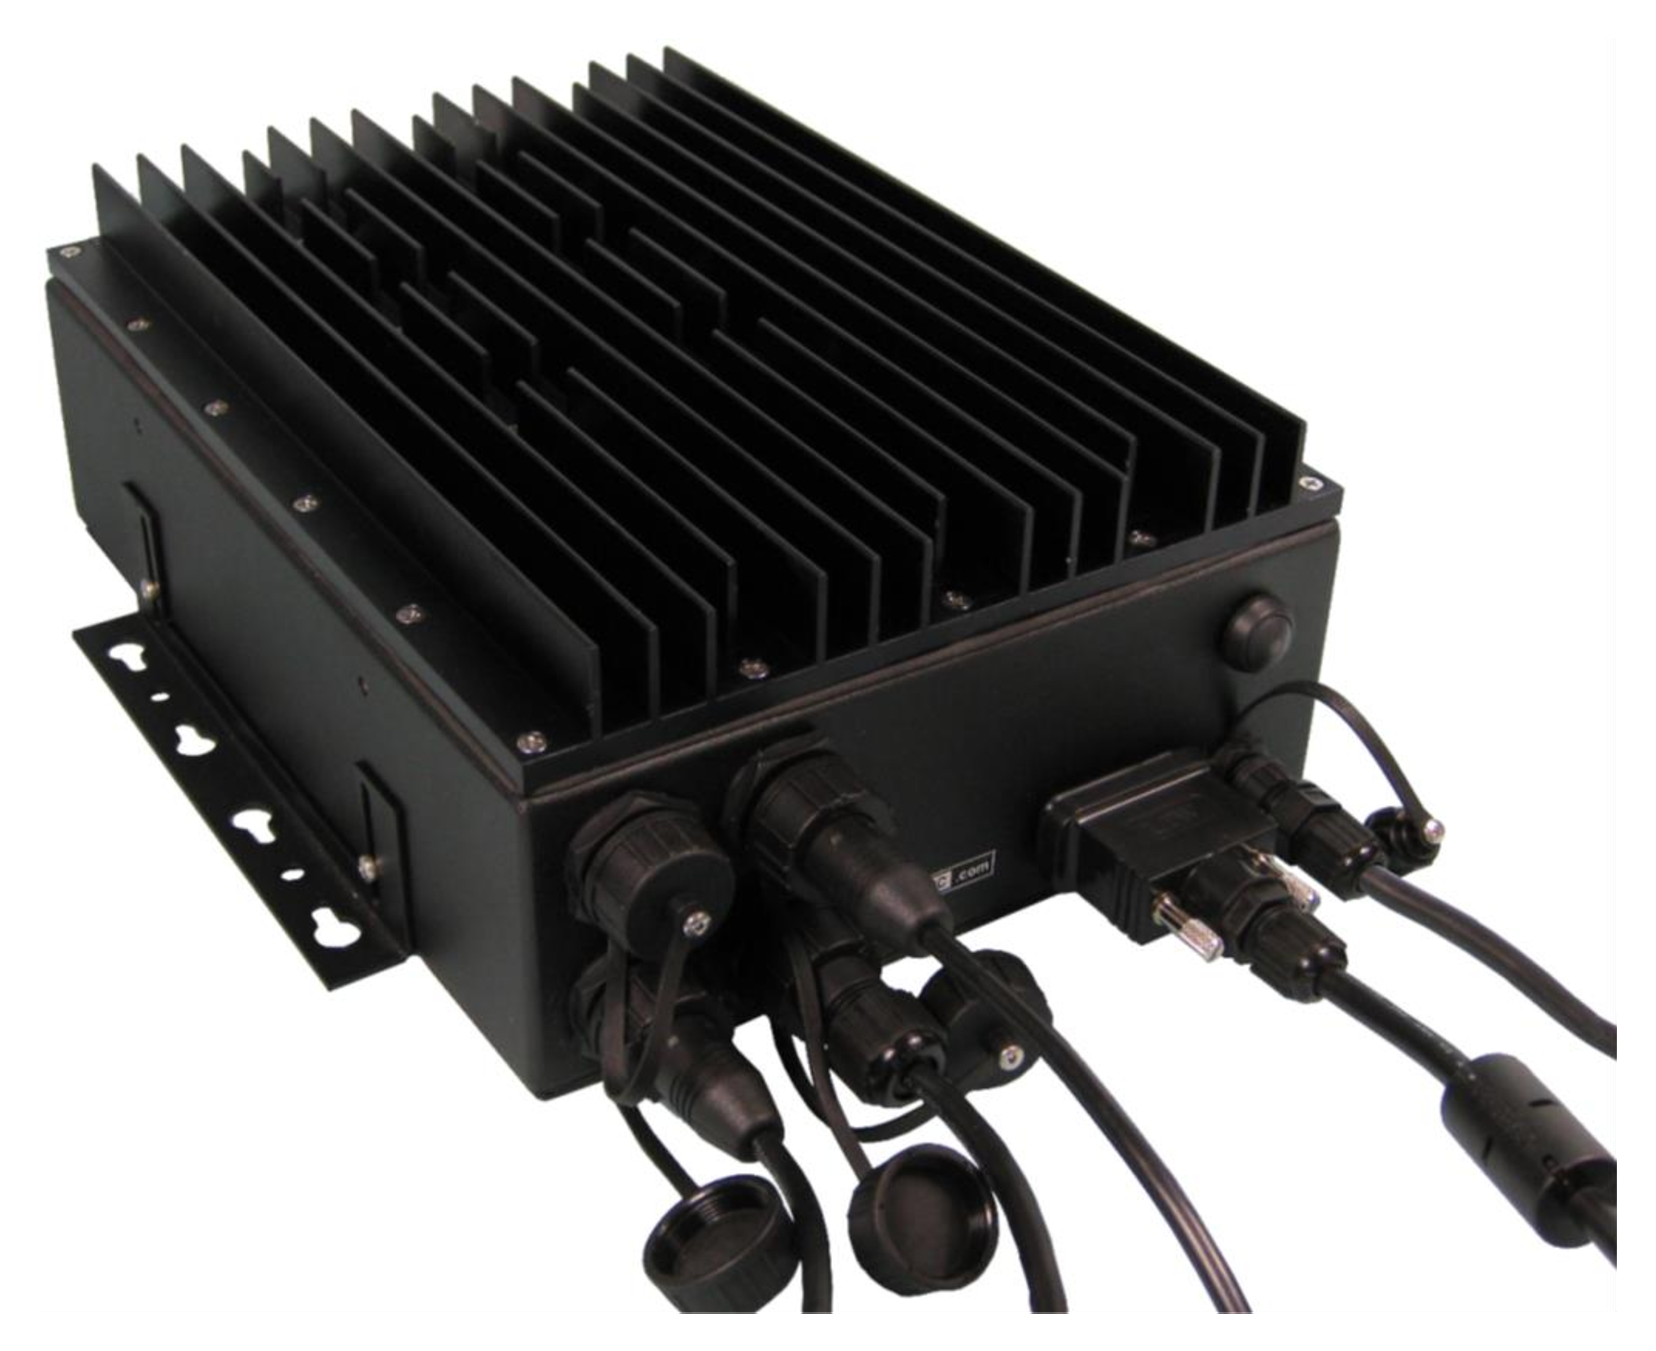
\includegraphics[angle=90,width=1\columnwidth]{figs/body02/FIGDEVICEPCOPTION3.pdf}\\
  \caption[Computer (Option 3): SC240ML-i724]{Computer (Option 3): SC240ML-i724}
  \label{FIG:DEVICEPCOPTION3}
\end{figure}
SC240ML-i724 cable set and heat pipe pictures can be seen in figure~\ref{FIG:DEVICEPCOPTION3CABLE}.
\begin{figure}
  \centering
  % Requires \usepackage{graphicx}
  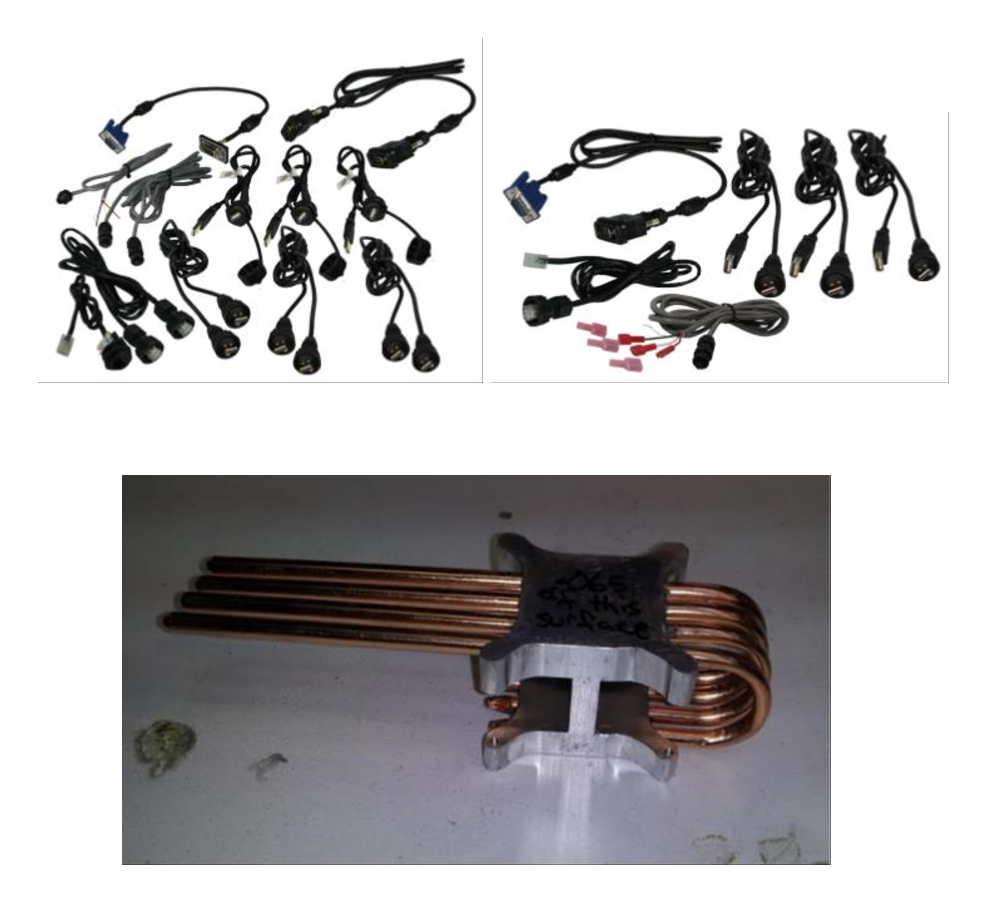
\includegraphics[angle=90,width=1\columnwidth]{figs/body02/FIGDEVICEPCOPTION3CABLE.pdf}\\
  \caption[Computer (Option 3): SC240ML-i724 cable set and heat pipe]{Computer (Option 3): SC240ML-i724 cable set and heat pipe}
  \label{FIG:DEVICEPCOPTION3CABLE}
\end{figure}
SC240ML-i724 technical drawing (in inches) using a specific customization can be seen in figure~\ref{FIG:DEVICEPCOPTION3DRAWING}.
\begin{figure}
  \centering
  % Requires \usepackage{graphicx}
  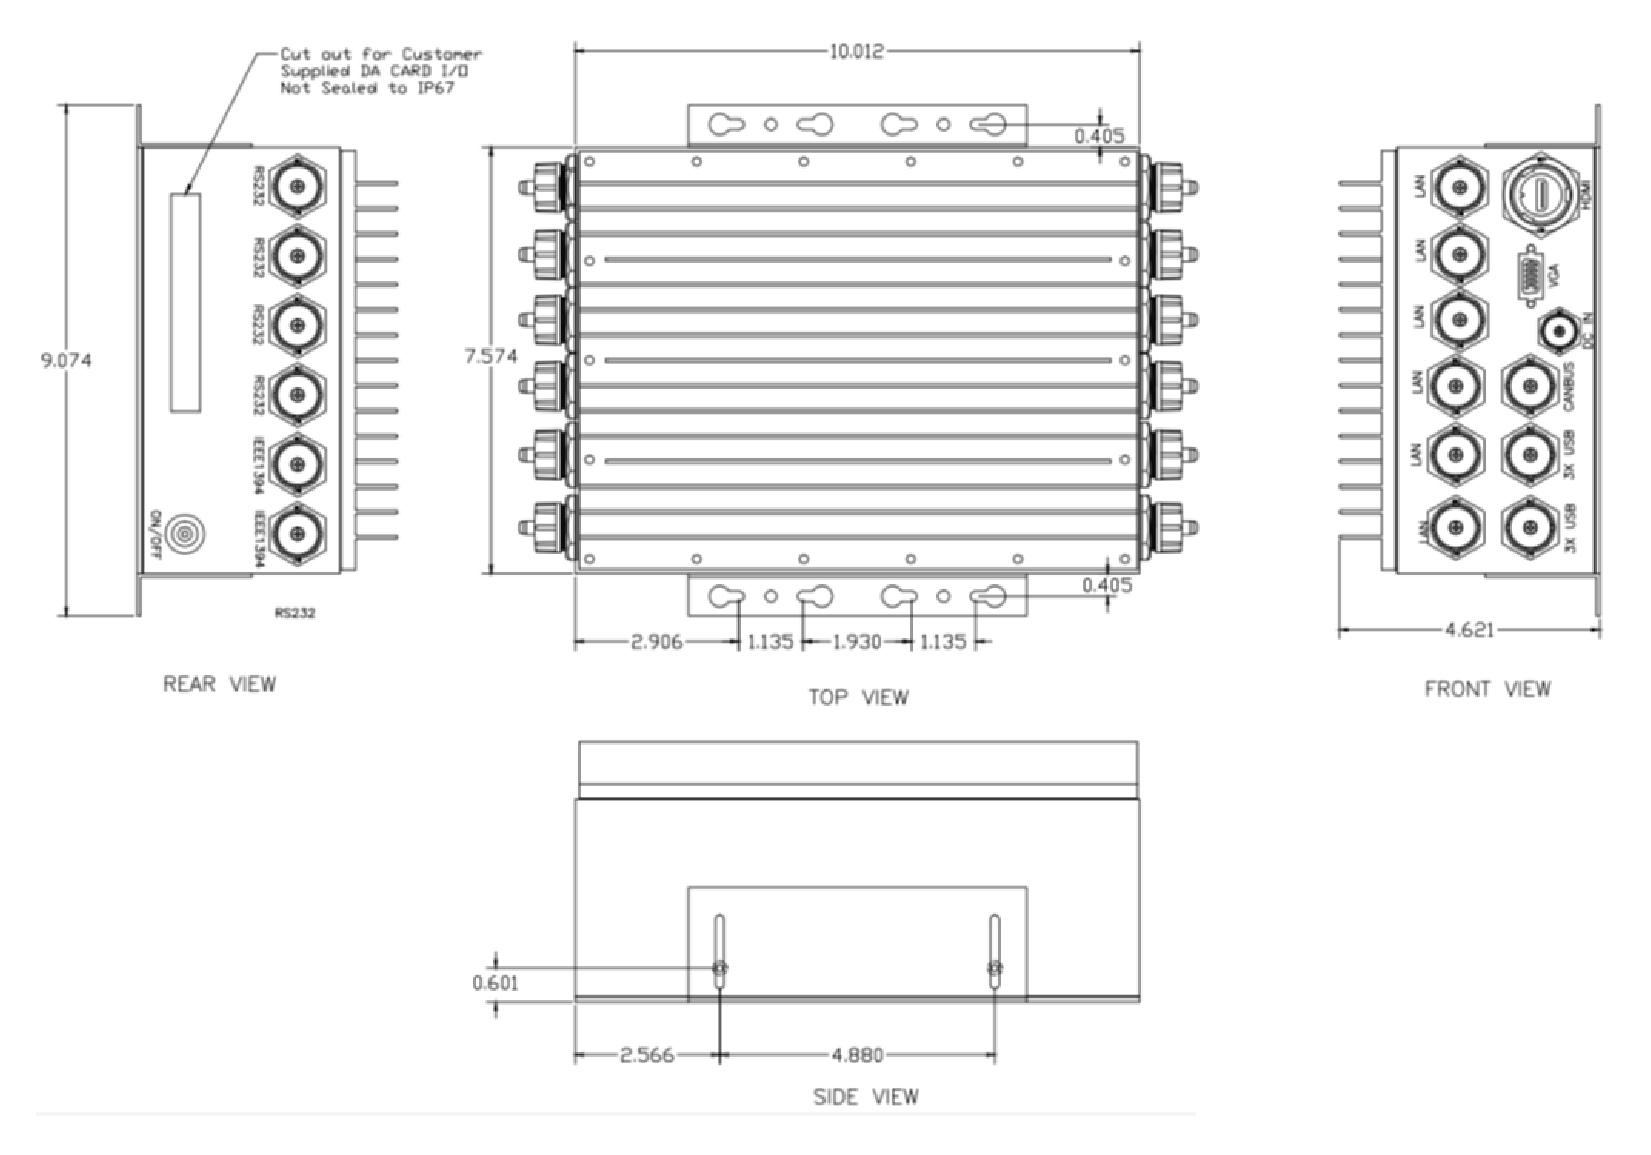
\includegraphics[angle=90,width=1\columnwidth]{figs/body02/FIGDEVICEPCOPTION3DRAWING.pdf}\\
  \caption[Computer (Option 3): SC240ML-i724 technical drawing (in inches)]{Computer (Option 3): SC240ML-i724 technical drawing (in inches)}
  \label{FIG:DEVICEPCOPTION3DRAWING}
\end{figure}

\section{Storage Devices} \label{DEVICE:STORAGE}
\section{1\textsuperscript{st} option: ESCREVER}

\section{Data acquisition system}

\section{Network devices} \label{DEVICE:NETWORK}
\subsection{Ethernet Switches}  \label{DEVICE:ETHERNETSWITCHES}
\subsection{1\textsuperscript{st} option: Korenix JetNet 3008G} \label{DEVICE:ETHERNETSWITCH3008G}
\begin{itemize}
  \item Manufacturer: Korenix
  \item Description:
  \begin{itemize}
    \item This Ethernet switch is an industrial product suitable for reliable Local Area Networks that demands high Ethernet speed. These objectives are achieved with its 8 Gigabit Ethernet ports, IP31 rugged aluminium case, Quality of Service (QoS) for packet forwarding and wide operating temperature (-10 to 70°C). In DORIS, it is suitable for use in modules 3 and 4, which can carry a great number of Ethernet devices.
  \end{itemize}
  \item Main features:
  \begin{itemize}
    \item Case: IP31 grade aluminum metal
    \item QoS: Compliance with IEEE802.1p class of service with Tag Based Priority. Each port support 4 priority queues with 8(Higher):4(High):2(Lo w):1(Lowest) scheduling. The Tag Priority ID as following: Higher (6,7), High (4,5), Low (0,3), Lowest (1,2)
    \item Operating Temperature: -10 to 70°C
    \item Storage Temperature: -40 to 85°C
    \item Power supply: 12-48VDC input range (nominal 24VDC)
    \item Power consumption: max 8W at 48VDC
    \item Approx. dimensions: 120mm x 55mm x 108mm
    \item Weight: 0.775kg with package, 0.525kg without package
  \end{itemize}
  \item Main interfaces:
  \begin{itemize}
    \item 8x (eight) Gigabit Ethernet 10/100/1000 Base-T(X) (female RJ-45)
  \end{itemize}
  \item Documentation:
  \begin{itemize}
    \item Website: \href{http://www.korenix.com/jetnet-ethernet-switch-3008G-overview.htm}{http://www.korenix.com/jetnet-ethernet-switch-3008G-overview.htm}
    \item Datasheet: see website.
    \item Manual: see website.
    \item Sales contact: sales@korenix.com; sales@korenix.com. For more info, see \href{http://www.korenix.com/contact-us.htm}{http://www.korenix.com/contact-us.htm}.
    \item Brazil sales: Marcelo.Reboucas@beijerinc.com; Flavio.Grassi@beijerinc.com. For more info, see \href{http://www.korenix.com/where-to-buy.htm}{http://www.korenix.com/where-to-buy.htm}.
  \end{itemize}
\end{itemize}
Korenix JetNet 3008G picture can be seen in figure~\ref{FIG:DEVICESWITCHOPTION1}.
\begin{figure}
  \centering
  % Requires \usepackage{graphicx}
  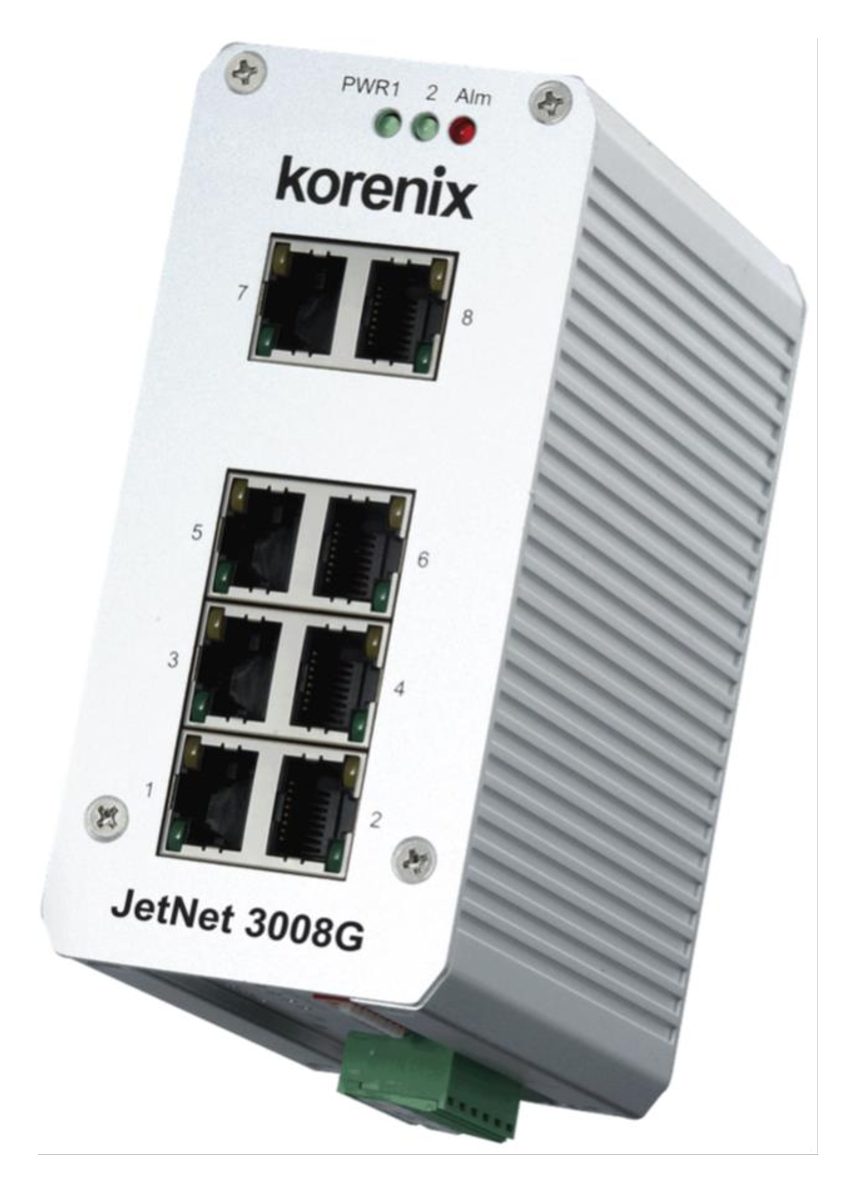
\includegraphics[angle=90,width=1\columnwidth]{figs/body02/FIGDEVICESWITCHOPTION1.pdf}\\
  \caption[Ethernet Switch (Option 1): Korenix JetNet 3008G]{Ethernet Switch (Option 1): Korenix JetNet 3008G}
  \label{FIG:DEVICESWITCHOPTION1}
\end{figure}
Korenix JetNet 3008G technical drawing (in millimeters) can be seen in figure~\ref{FIG:DEVICESWITCHOPTION1DRAWING}.
\begin{figure}
  \centering
  % Requires \usepackage{graphicx}
  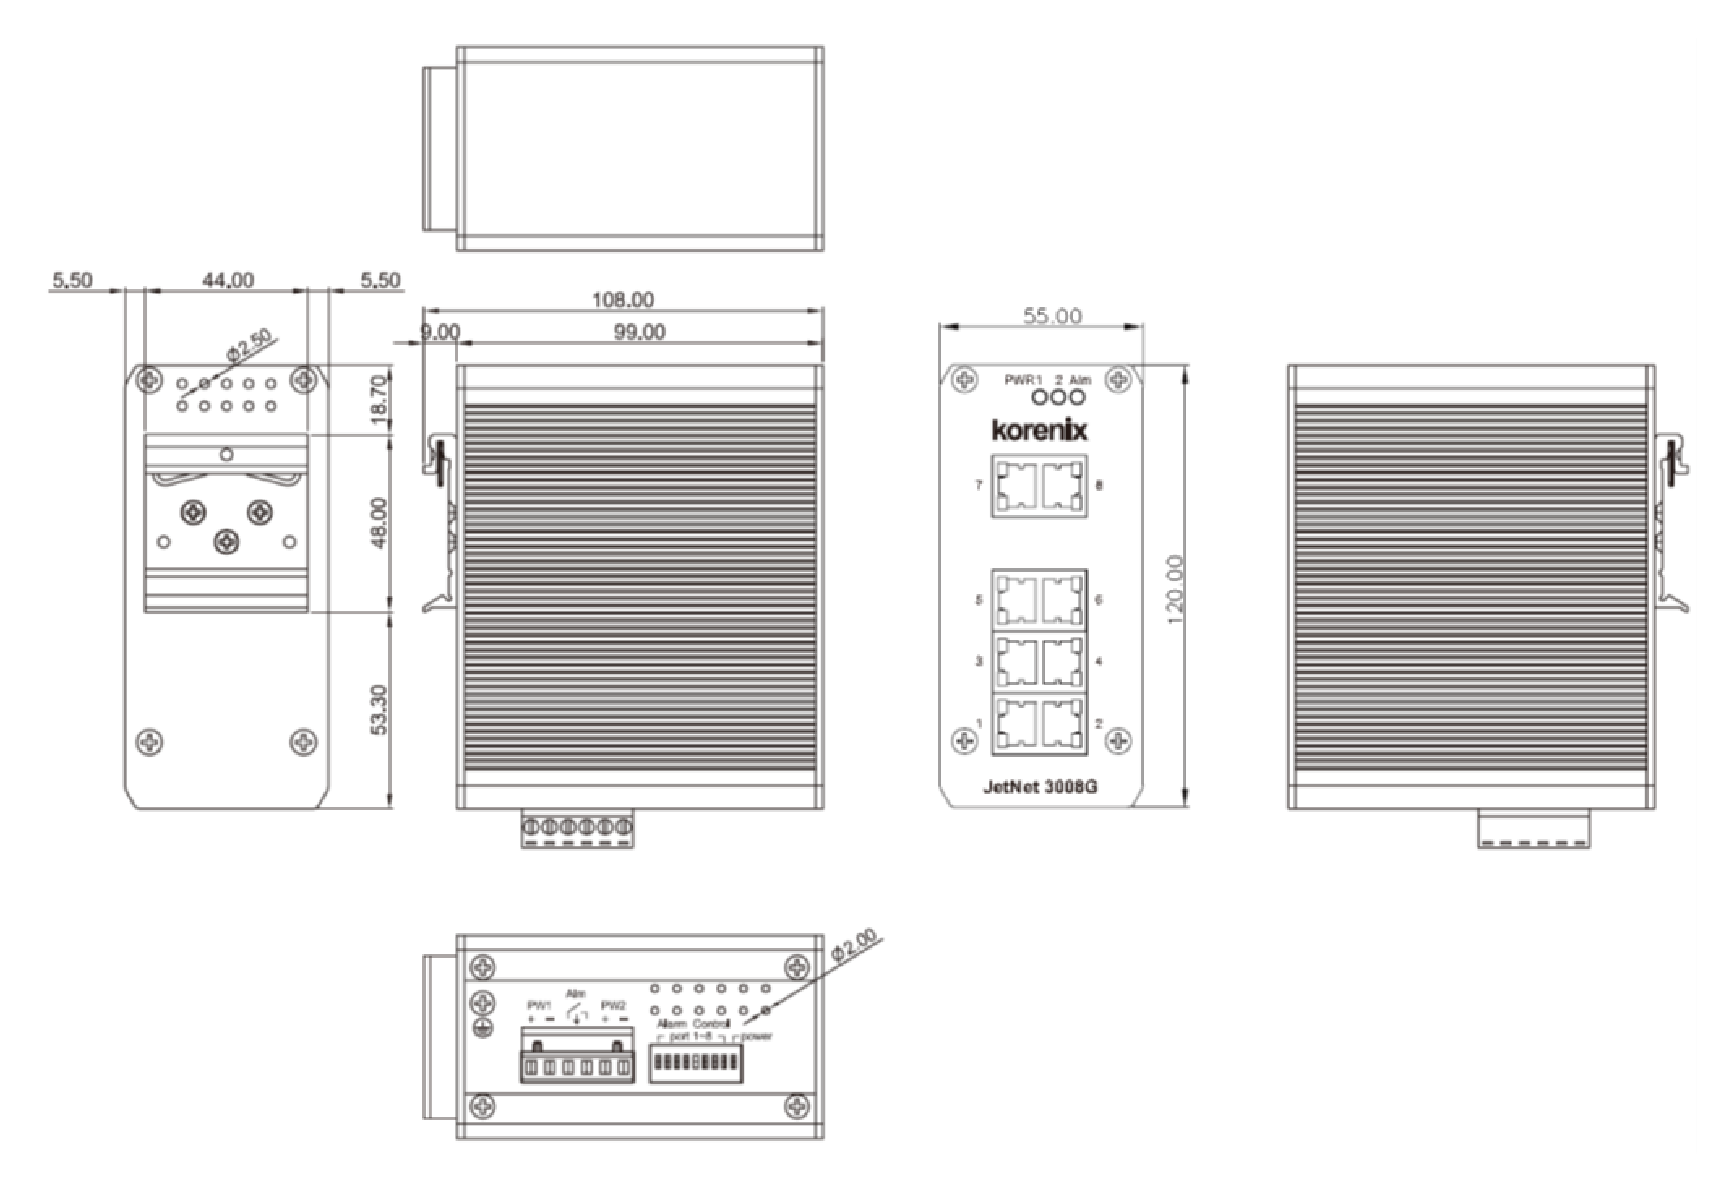
\includegraphics[angle=90,width=1\columnwidth]{figs/body02/FIGDEVICESWITCHOPTION1DRAWING.pdf}\\
  \caption[Ethernet Switch (Option 1): Korenix JetNet 3008G technical drawing (in inches)]{Ethernet Switch (Option 1): Korenix JetNet 3008G technical drawing (in inches)}
  \label{FIG:DEVICESWITCHOPTION1DRAWING}
\end{figure}


\subsection{2\textsuperscript{nd} option: Korenix JetNet 3005G} \label{DEVICE:ETHERNETSWITCH3005G}
\begin{itemize}
  \item Manufacturer: Korenix
  \item Description:
  \begin{itemize}
    \item This Ethernet switch is similar to the first option above, except that this model has only five ports. Hence, it is suitable for use in DORIS modules 1 and 2, which carry a few number of Ethernet devices.
  \end{itemize}
  \item Main features:
  \begin{itemize}
    \item Case: IP31 grade aluminum metal
    \item QoS: Compliance with IEEE802.1p class of service with Tag Based Priority. Each port support 4 priority queues with 8(Higher):4(High):2(Lo w):1(Lowest) scheduling. The Tag Priority ID as following: Higher (6,7), High (4,5), Low (0,3), Lowest (1,2)
    \item Operating Temperature: -10 to 70°C
    \item Storage Temperature: -40 to 85°C
    \item Power supply: 12-48VDC input range (nominal 24VDC)
    \item Power consumption: max 8W at 48VDC
    \item Approx. dimensions: 120mm x 55mm x 108mm
    \item Weight: 0.775kg with package, 0.525kg without package
  \end{itemize}
  \item Main interfaces:
  \begin{itemize}
    \item 5x (eight) Gigabit Ethernet 10/100/1000 Base-T(X) (female RJ-45)
  \end{itemize}
  \item Documentation:
  \begin{itemize}
    \item Website: \href{http://www.korenix.com/jetnet-ethernet-switch-3005G-overview.htm}{http://www.korenix.com/jetnet-ethernet-switch-3005G-overview.htm}
    \item Datasheet: see website.
    \item Manual: see website.
    \item Sales contact: sales@korenix.com; sales@korenix.com. For more info, see \href{http://www.korenix.com/contact-us.htm}{http://www.korenix.com/contact-us.htm}.
    \item Brazil sales (Beijer Brasil): Marcelo.Reboucas@beijerinc.com; Flavio.Grassi@beijerinc.com. For more info, see \href{http://www.korenix.com/where-to-buy.htm}{http://www.korenix.com/where-to-buy.htm}.
  \end{itemize}
\end{itemize}
Korenix JetNet 3005G picture can be seen in figure~\ref{FIG:DEVICESWITCHOPTION2}.
\begin{figure}
  \centering
  % Requires \usepackage{graphicx}
  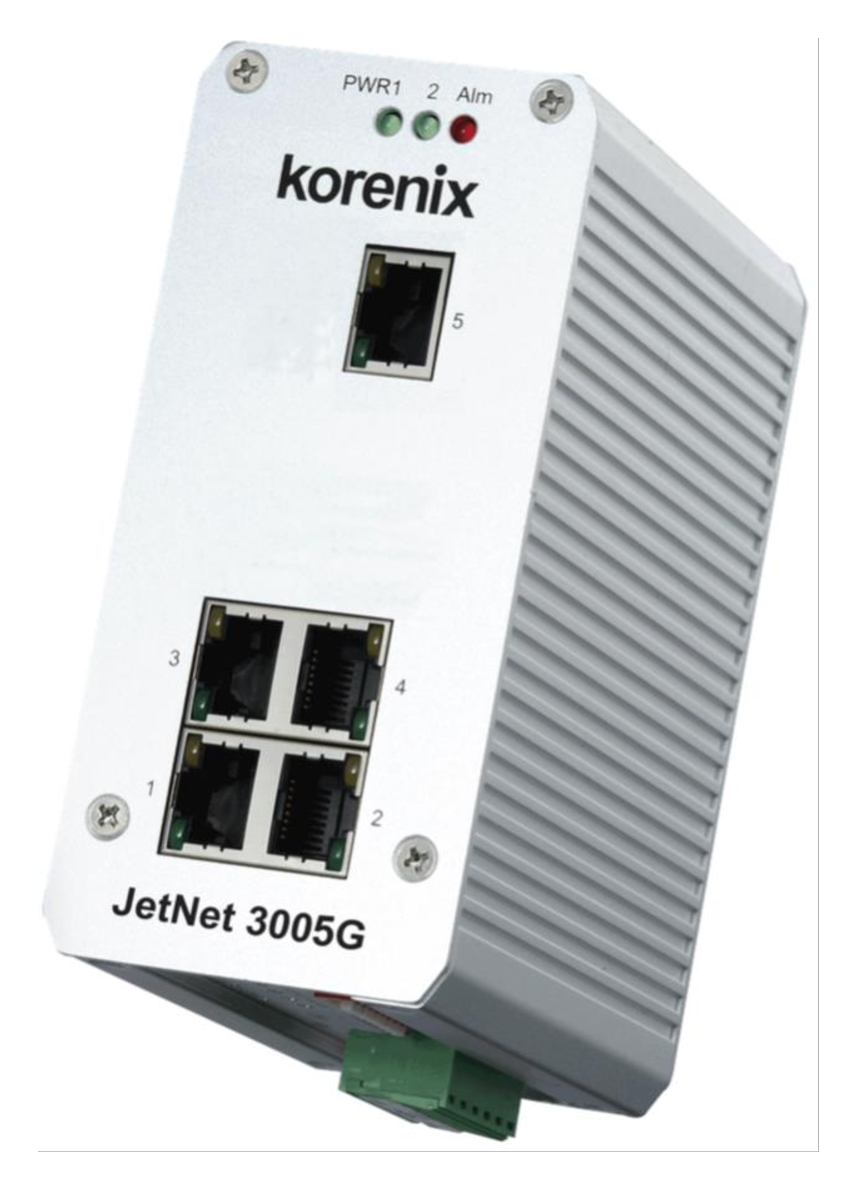
\includegraphics[angle=90,width=1\columnwidth]{figs/body02/FIGDEVICESWITCHOPTION2.pdf}\\
  \caption[Ethernet Switch (Option 2): Korenix JetNet 3008G]{Ethernet Switch (Option 2): Korenix JetNet 3005G}
  \label{FIG:DEVICESWITCHOPTION2}
\end{figure}
Korenix JetNet 3005G technical drawing (in millimeters) can be seen in figure~\ref{FIG:DEVICESWITCHOPTION2DRAWING}.
\begin{figure}
  \centering
  % Requires \usepackage{graphicx}
  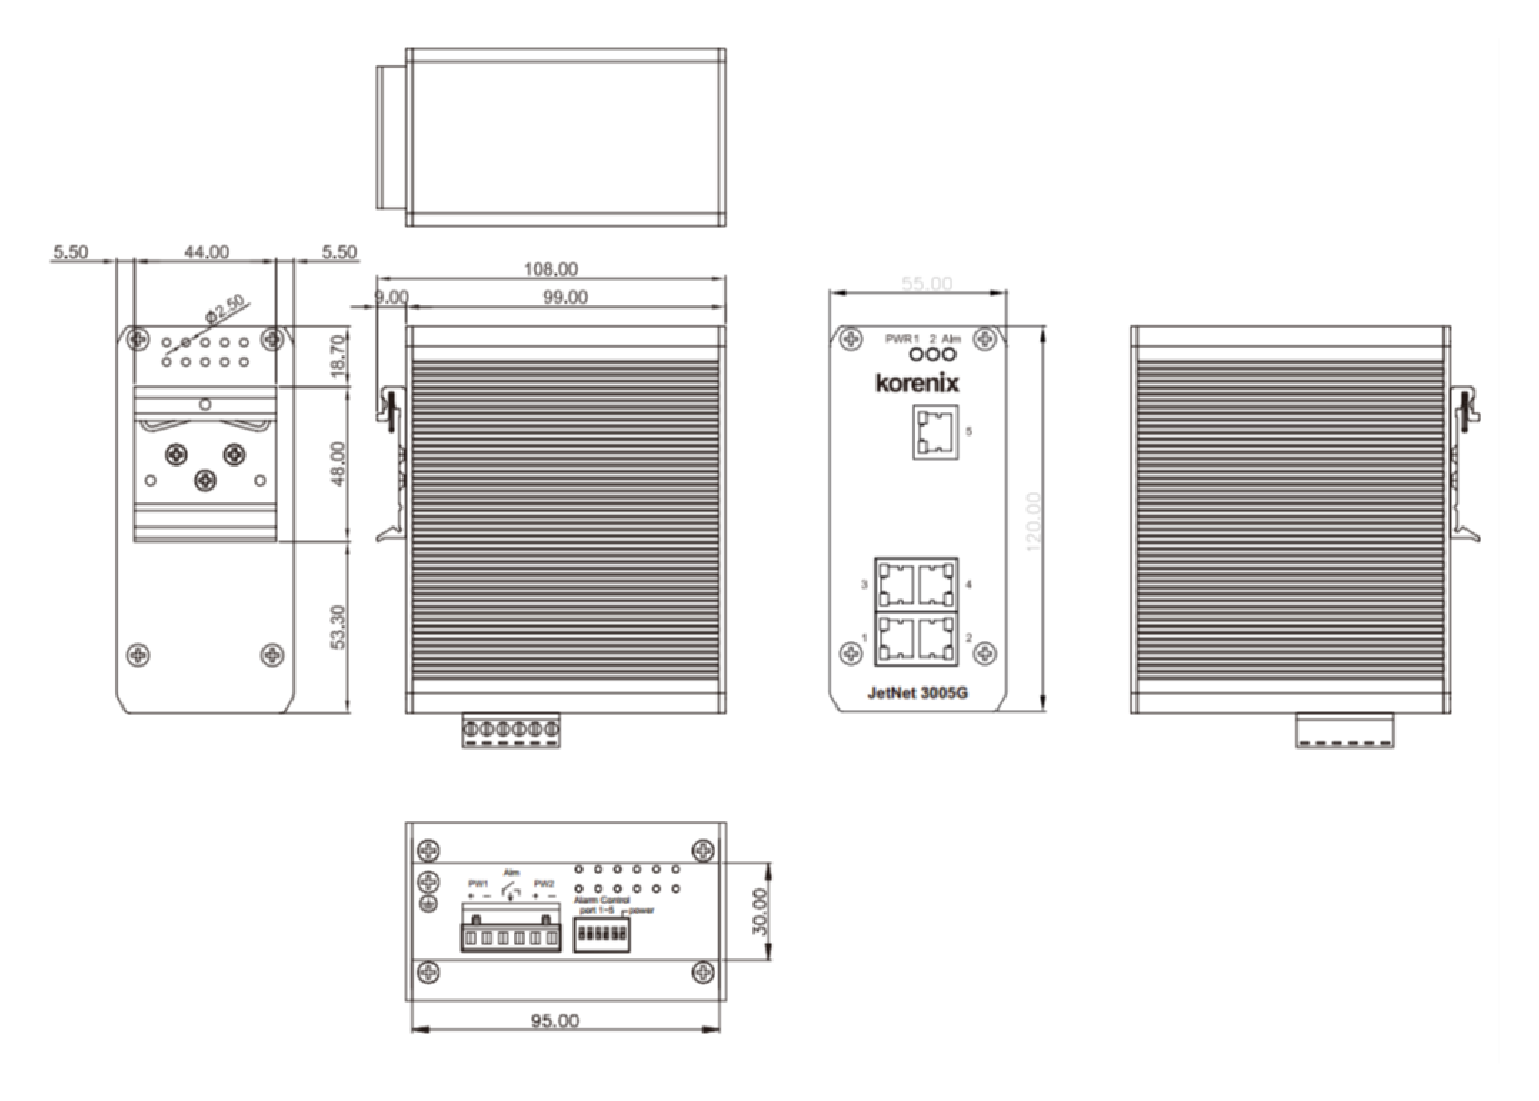
\includegraphics[angle=90,width=1\columnwidth]{figs/body02/FIGDEVICESWITCHOPTION2DRAWING.pdf}\\
  \caption[Ethernet Switch (Option 2): Korenix JetNet 3005G technical drawing (in inches)]{Ethernet Switch (Option 2): Korenix JetNet 3005G technical drawing (in inches)}
  \label{FIG:DEVICESWITCHOPTION2DRAWING}
\end{figure}


\subsection{3\textsuperscript{rd} option: Korenix JetNet 3005G V2} \label{DEVICE:ETHERNETSWITCH3005GV2}
\begin{itemize}
  \item Manufacturer: Korenix
  \item Description:
  \begin{itemize}
    \item This Ethernet switch is similar to the second option above. However, this model is smaller, which makes it suitable for DORIS, since the robot inside devices must be as smaller as possible. This is an ultimate model from Korenix, still not available for purchase.
  \end{itemize}
  \item Information:
  \begin{itemize}
    \item Website: \href{http://www.korenix.com/jetnet-ethernet-switch-3005G-V2-overview.htm}{http://www.korenix.com/jetnet-ethernet-switch-3005G-V2-overview.htm}
    \item Sales contact: sales@korenix.com; sales@korenix.com. For more info, see \href{http://www.korenix.com/contact-us.htm}{http://www.korenix.com/contact-us.htm}.
    \item Brazil sales: Marcelo.Reboucas@beijerinc.com; Flavio.Grassi@beijerinc.com. For more info, see \href{http://www.korenix.com/where-to-buy.htm}{http://www.korenix.com/where-to-buy.htm}.
  \end{itemize}
\end{itemize}
Korenix JetNet 3008G picture can be seen in figure~\ref{FIG:DEVICESWITCHOPTION3}.
\begin{figure}
  \centering
  % Requires \usepackage{graphicx}
  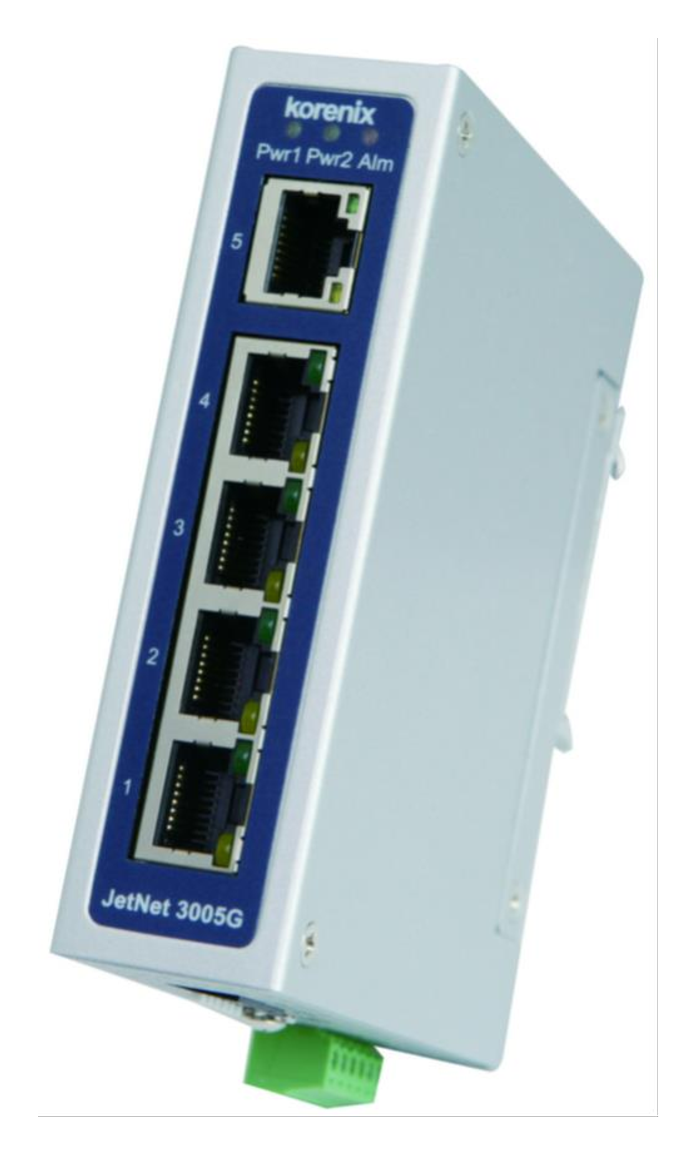
\includegraphics[angle=90,width=1\columnwidth]{figs/body02/FIGDEVICESWITCHOPTION3.pdf}\\
  \caption[Ethernet Switch (Option 3): Korenix JetNet 3005G V2]{Ethernet Switch (Option 3): Korenix JetNet 3005G V2}
  \label{FIG:DEVICESWITCHOPTION3}
\end{figure}


\subsection{4\textsuperscript{th} option: Korenix JetNet 5010G-w} \label{DEVICE:ETHERNETSWITCH5010G}
\begin{itemize}
  \item Manufacturer: Korenix
  \item Description:
  \begin{itemize}
    \item This Ethernet switch model belongs to the same family of the above options. However, the previous models are not managed switch, and the QoS setting depends on which port each network branch is connected. On the other hand, the model Korenix JetNet 5010G-w is equipped with a managed QoS system (QoS in Layer 3 TOS/DiffServ), which allows the visualization and optimization of data traffic via software, hence improving the network speed and performance. In general, the managed Ethernet Switches models found in the market are extremely big and heavy, and few models have Gigabit speed at all ports. The model Korenix JetNet 5010G-w offers a trade-off between size, weight and number of Gigabit Ethernet ports.
  \end{itemize}
  \item Main features:
  \begin{itemize}
    \item Case: IP31 protection, aluminum metal case
    \item QoS: Four priority queues per port, IEEE802.1p COS and Layer 3 TOS/DiffServ
    \item Operating Temperature: -40 to 75°C
    \item Storage Temperature: -40 to 85°C
    \item Power supply: 10.5-60VDC input range (nominal 24VDC)
    \item Power consumption: max 8W at 48VDC
    \item Approx. dimensions: 137mm x 96mm x 119mm
    \item Weight: 0.915kg with package
  \end{itemize}
  \item Main interfaces:
  \begin{itemize}
    \item 7x 10/100TX (Fast Ethernet) RJ-45
    \item 3x 10/100/1000TX (Gigabit Ethernet) RJ-45 combo with SFP
    \item Gigabit Fiber/100Base-FX: 3 x SFP with Hot Swappable
  \end{itemize}
  \item Documentation:
  \begin{itemize}
    \item Website: \href{http://www.korenix.com/jetnet-ethernet-switch-5010G-overview.htm}{http://www.korenix.com/jetnet-ethernet-switch-5010G-overview.htm}
    \item Datasheet: see website.
    \item Manual: see website.
    \item Sales contact: sales@korenix.com; sales@korenix.com. For more info, see \href{http://www.korenix.com/contact-us.htm}{http://www.korenix.com/contact-us.htm}.
    \item Brazil sales (Beijer Brasil): Marcelo.Reboucas@beijerinc.com; Flavio.Grassi@beijerinc.com. For more info, see \href{http://www.korenix.com/where-to-buy.htm}{http://www.korenix.com/where-to-buy.htm}.
  \end{itemize}
\end{itemize}
Korenix JetNet 3010G-w picture can be seen in figure~\ref{FIG:DEVICESWITCHOPTION4}.
\begin{figure}
  \centering
  % Requires \usepackage{graphicx}
  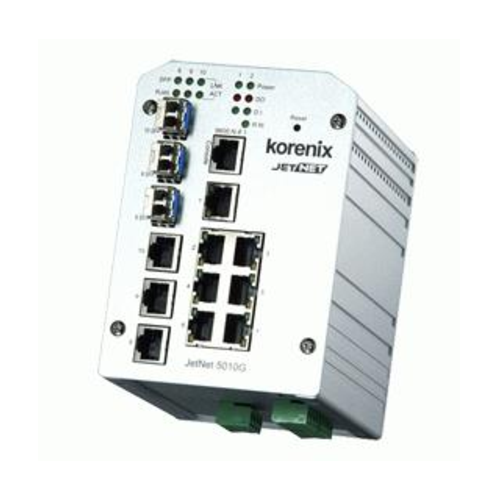
\includegraphics[angle=90,width=1\columnwidth]{figs/body02/FIGDEVICESWITCHOPTION4.pdf}\\
  \caption[Ethernet Switch (Option 4): Korenix JetNet 3010G-w]{Ethernet Switch (Option 4): Korenix JetNet 3010G-w}
  \label{FIG:DEVICESWITCHOPTION4}
\end{figure}
Korenix JetNet 3010G-w technical drawing (in millimeters) can be seen in figure~\ref{FIG:DEVICESWITCHOPTION4DRAWING}.
\begin{figure}
  \centering
  % Requires \usepackage{graphicx}
  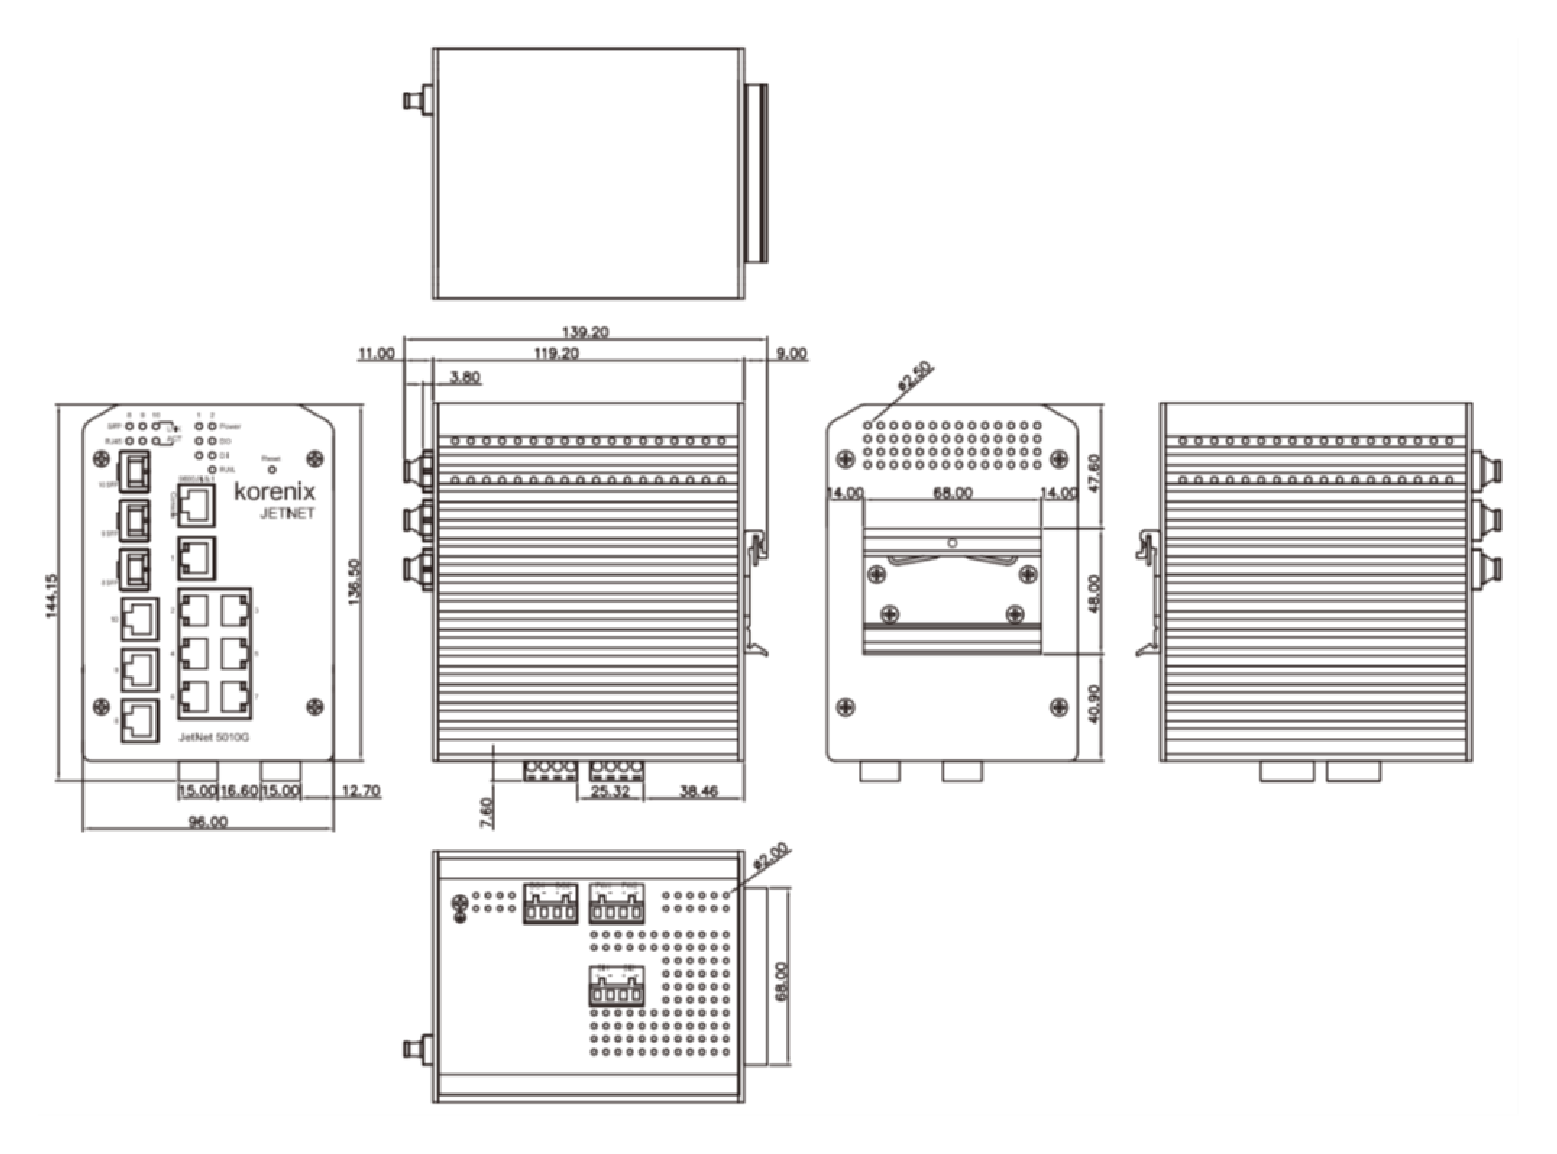
\includegraphics[angle=90,width=1\columnwidth]{figs/body02/FIGDEVICESWITCHOPTION4DRAWING.pdf}\\
  \caption[Ethernet Switch (Option 4): Korenix JetNet 3010G-w technical drawing (in inches)]{Ethernet Switch (Option 4): Korenix JetNet 3010G-w technical drawing (in inches)}
  \label{FIG:DEVICESWITCHOPTION4DRAWING}
\end{figure}
\subsection{Wi-Fi Access Points}  \label{DEVICE:WIFI}
\subsection{1\textsuperscript{st} option: EXTRONICS Universal Zone 1 Access Point Enclosure iWAP107} \label{DEVICE:iWAP107}
\begin{itemize}
  \item Manufacturer: Extronics
  \item Description:
  \begin{itemize}
    \item This Access point provides Wi-Fi IEEE 802.11n/ac and 1 Gigabit Ethernet port. The standard IEEE 802.11n/ac can provide a maximum of 300 Mbit rate for wireless. This product also complies with ATEX and IECEx certification, which meets the requirement for safe operation in classified Zone 1. According to ATEX certification for this model, the compliance with the Essential Health and Safety Requirements has been assured by compliance with EN60079 standards, specially EN60079-11:2012, which defines an intrinsically safe (Ex i) operation by the definition of RF EIRP allowed limitations in hazardous areas. This is achieved by using an embedded device (Extronics iSOLATE500 RF, see section~\ref{DEVICE:iSOLATE500RF} for more info.), which makes all the antenna points intrinsically safe.Furthermore, this product meets explosion proof (Ex d) requirements. As iWAP107 has an special Ex d enclosure, it is considerably heavy for use in vehicle applications.
  \end{itemize}
  \item Main features:
  \begin{itemize}
    \item Case: marine grade cooper free aluminum light alloy, epoxy powder coated (IP66 protection)
    \item Operating Temperature: -40 to 60°C
    \item Power supply: DC (unknown voltage)
    \item Power consumption: 25W (basic configuration), 125W (with heaters)
    \item Approx. dimensions: 415mm x 315mm x 250mm
    \item Approx. weight: 30 kg
  \end{itemize}
  \item Main interfaces:
  \begin{itemize}
    \item 1x (one) Gigabit Ethernet 100/1000 Base-T
    \item Wi-Fi (802.11n/ac) customizable antennas
  \end{itemize}
  \item Customization:
  \begin{itemize}
    \item For DORIS, the ideal customization requires 4 antennas for ESCREVER.
  \end{itemize}
  \item Documentation:
  \begin{itemize}
    \item Website: \href{http://www.extronics.com/wireless/zone\_1\_\_21\_wireless\_access\_points/iwap107}{http://www.extronics.com/wireless/zone\_1\_\_21\_wireless\_access\_points/iwap107}
    \item Datasheet: see website.
    \item Manual: see website.
    \item Certifications: see website.
    \item Sales contact: info@extronics.com; karen.bentley@extronics.com; james.eastwood@extronics.com. For more info, see \href{http://www.extronics.com/contact\_us}{http://www.extronics.com/contact\_us}.
  \end{itemize}
\end{itemize}
Extronics iWAP107 picture can be seen in figure~\ref{FIG:DEVICEWIFIOPTION1}.
\begin{figure}
  \centering
  % Requires \usepackage{graphicx}
  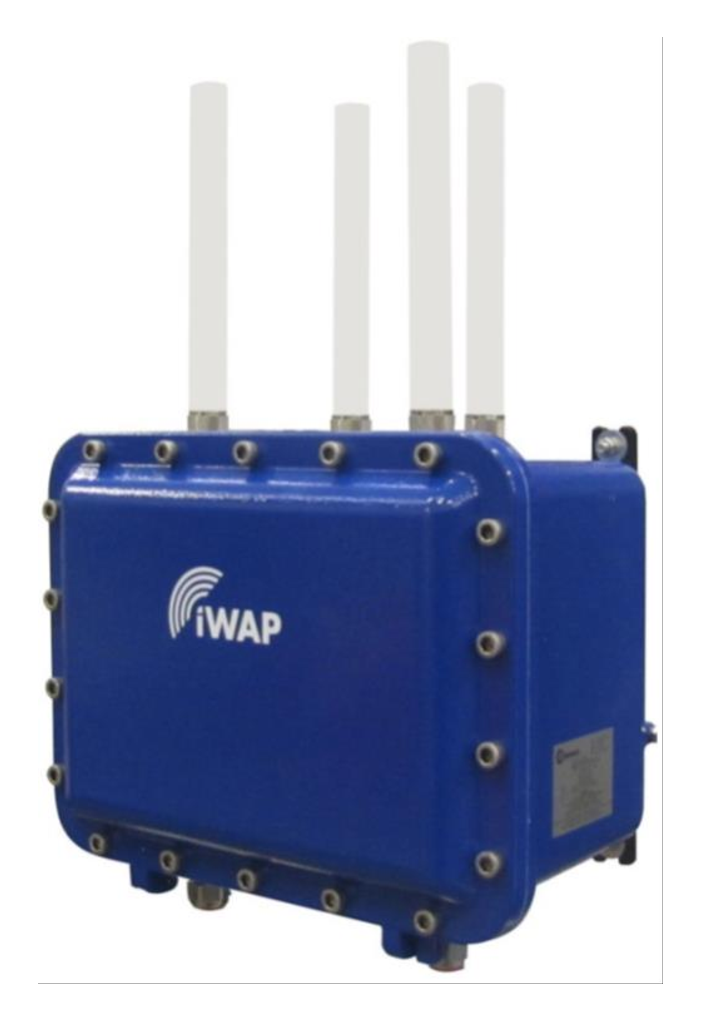
\includegraphics[angle=90,width=1\columnwidth]{figs/body02/FIGDEVICEWIFIOPTION1.pdf}\\
  \caption[Wi-Fi Access Point (Option 1): Extronics iWAP107]{Wi-Fi Access Point (Option 1): Extronics iWAP107}
  \label{FIG:DEVICEWIFIOPTION1}
\end{figure}
\subsection{CAN devices} \label{DEVICE:CAN}
\section{Traction devices}
\subsection{Motors}
\subsubsection{1\textsuperscript{st} option: Maxon Motor EC-4pole 30 diam 30 mm, brushless, 200 Watt Part Number: 305013} \label{DEVICE:MOTOR1}
\begin{itemize}
  \item Manufacturer: Maxon Motor
  \item Description:
  \begin{itemize}
    \item This EC brushless motor was specified by mechanics team (G1) with the aid guidelines of the electronics team (G2). Its main features (output power/torque, maximum electric current, efficiency, thermal constant etc.) satisfy both mechanical and electronics project requirements for DORIS traction system, which demands 4 motors.
  \end{itemize}
  \item Main features:
  \begin{itemize}
    \item Nominal speed: 15900 rpm
    \item Nominal torque: (max. continuous torque) 135 mNm
    \item Nominal current: (max. continuous current) 10.5 A
    \item Max. efficiency: 89\%
    \item Torque constant: 13.6 mNm/A
    \item Ambient temperature: -20 to 100 °C
    \item Number of pole pairs:	2
    \item Thermal constant: 2.11s
    \item Weight: 300g
  \end{itemize}
  \item Documentation:
  \begin{itemize}
    \item Website: \href{http://www.maxonmotor.com/maxon/view/product/motor/ecmotor/ec4pole/305013}{http://www.maxonmotor.com/maxon/view/product/motor/ecmotor/ec4pole/305013}
    \item Datasheet: see website.
    \item Manual: see website.
    \item Sales contact: see G1 project.
  \end{itemize}
\end{itemize}
Maxon Motor EC-4pole 200W 305013 picture can be seen in figure~\ref{FIG:DEVICEMOTOROPTION1}.
\begin{figure}
  \centering
  % Requires \usepackage{graphicx}
  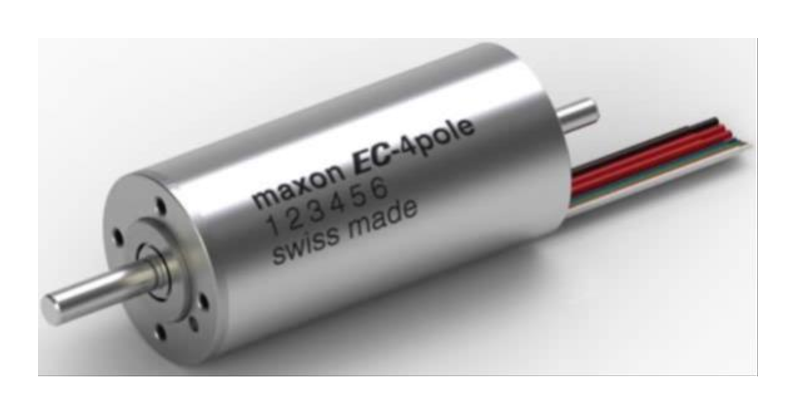
\includegraphics[angle=90,width=1\columnwidth]{figs/body02/FIGDEVICEMOTOROPTION1.pdf}\\
  \caption[Motor (Option 1): Maxon Motor EC-4pole 200W 305013]{Motor (Option 1): Maxon Motor EC-4pole 200W 305013}
  \label{FIG:DEVICEMOTOROPTION1}
\end{figure}
\subsection{Encoders}
\subsubsection{1\textsuperscript{st} option: Maxon Motor Encoder MR, Type ML, 500 CPT, 3 Channels, with Line Driver Part Number: 225778} \label{DEVICE:ENCODER1}
\begin{itemize}
  \item Manufacturer: Maxon Motor
  \item Description:
  \begin{itemize}
    \item This encoder was specified by mechanics team (G1) with the aid guidelines of the electronics team (G2). Its main features satisfy both mechanical and electronics project requirements for DORIS traction system, which demands an encoder for each of the 4 motors. This encoder should be used together with the motor 1\textsuperscript{st} option (see section above).
  \end{itemize}
  \item Main features:
  \begin{itemize}
    \item Counts per turn: 500
    \item Number of channels: 3
    \item Max. mechanical speed: 24000 rpm
    \item Supply voltage Vcc: 4.7. to 5.2VDC
    \item Index synchronized to AB: No
    \item Operating temperature: -25 to 85 °C
  \end{itemize}
  \item Documentation:
  \begin{itemize}
    \item Website: \href{http://www.maxonmotor.com/maxon/view/product/sensor/encoder/Encoder-MR-TypML-128-1000imp-3Kanal/225778}{http://www.maxonmotor.com/maxon/view/product/sensor/encoder/Encoder-MR-TypML-128-1000imp-3Kanal/225778}
    \item Datasheet: see website.
    \item Manual: see website.
    \item Sales contact: see G1 project.
  \end{itemize}
\end{itemize}
\subsection{Reduction gears}
\subsubsection{1\textsuperscript{st} option: Maxon Motor Planetary Gearhead GP 32 HP diam 32 mm, 4.0 - 8.0 Nm, Metal Version, High Power Part Number: 326660} \label{DEVICE:GEAR1}
\begin{itemize}
  \item Manufacturer: Maxon Motor
  \item Description:
  \begin{itemize}
    \item This reduction gear was specified by mechanics team (G1). Its reduction factor (21:1) satisfy mechanical parameters for the traction module project.
  \end{itemize}
  \item Main features:
  \begin{itemize}
    \item Reduction: 21:1
    \item Absolute reduction: 299:14
    \item Outer diameter: 32 mm
    \item Number of stages: 2
    \item Max. continuous torque: 4 Nm
    \item Max. intermittent torque: 6 Nm
    \item Max. transmittable power (continuous): 160 W
    \item Max. transmittable power (intermittent): 240 W
    \item Weight: 170g
  \end{itemize}
  \item Documentation:
  \begin{itemize}
    \item Website: \href{http://www.maxonmotor.com/maxon/view/product/gear/planetary/gp32/326660}{http://www.maxonmotor.com/maxon/view/product/gear/planetary/gp32/326660}
    \item Datasheet: see website.
    \item Manual: see website.
    \item Sales contact: see G1 project.
  \end{itemize}
\end{itemize}
Maxon Motor Planetary Gearhead 21:1 326660 picture can be seen in figure~\ref{FIG:DEVICEEARGOPTION1}.
\begin{figure}
  \centering
  % Requires \usepackage{graphicx}
  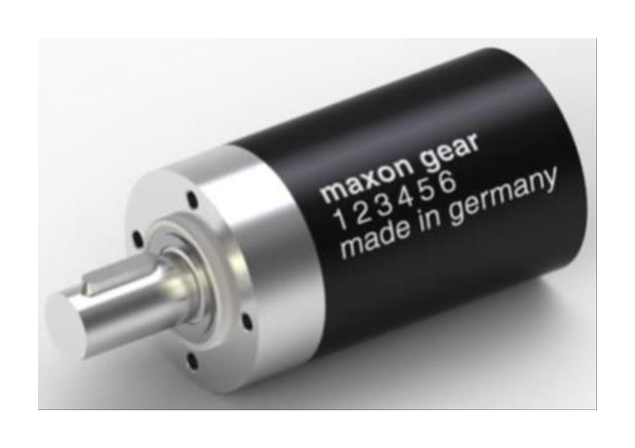
\includegraphics[angle=90,width=1\columnwidth]{figs/body02/FIGDEVICEGEAROPTION1.pdf}\\
  \caption[Reduction gear (Option 1): Maxon Motor Planetary Gearhead 21:1 326660]{Reduction gear (Option 1): Maxon Motor Planetary Gearhead 21:1 326660}
  \label{FIG:DEVICEGEAROPTION1}
\end{figure}
\subsection{Controller drivers}
\subsubsection{1\textsuperscript{st} option: Maxon Motor EPOS2 70/10, Digital positioning controller, 10 A, 11 - 70 VDC Part Number: 375711} \label{DEVICE:DRIVER1}
\begin{itemize}
  \item Manufacturer: Maxon Motor
  \item Description:
  \begin{itemize}
    \item This controller driver was specified by mechanics team (G1) with the aid guidelines of the electronics team (G2). Its main features (power supply range, max. output current/tension, CAN/USB interfaces, etc.) satisfy both mechanical and electronics project requirements for DORIS traction system, which demands 4 EC motors like the model described in section~\ref{DEVICE:MOTOR1}.
  \end{itemize}
  \item Main features:
  \begin{itemize}
    \item EC motors: up to 700W
    \item Supports Digital Incremental Encoder (3 channel, differential)
    \item Supports Digital Hall Sensors (EC Motors)
    \item Performs Current/Speed/Position control
    \item Operating voltage Vcc: 11VDC to 70VDC
    \item Max. output current: 25A
    \item Max. time of peak output current: 1s
    \item Continuous output current: 10A
    \item Max. efficiency: 94\%
    \item Hall sensor signals: H1, H2, H2
    \item Encoder signals: A, A/, B, B/, I, I/
    \item Digital inputs: 10
    \item Functionality of the digital inputs: limit switch, reference switch, general purpose, enable, quickstop, SSI encoder, 2nd incremental encoder, step/direction set value, master encoder, position marker, power stage enable
    \item Analog inputs: 2
    \item DIP switch: 8
    \item Functionality of the DIP switch: set CAN Node-ID, set CAN-Bus Termination
    \item Digital outputs: 5
    \item Functionality of the digital outputs: holding brake, general purpose, position compare, ready
    \item Hall sensor supply voltage: 5VDC, max. 30mA
    \item Encoder supply voltage: 5VDC, max. 100mA
    \item Interfaces: RS232/USB 2.0/CAN (CAN Open Software)
    \item Graphical User Interface: EPOS Studio
    \item Status indicator READY: green LED
    \item Status indicator ERROR: red LED
    \item Operation temperature: -10 to 45°C
    \item Storage temperature: -40 to 85°C
    \item Dimensions: 150mm x 93mm x 27mm
    \item Weight: 330g
  \end{itemize}
  \item Documentation:
  \begin{itemize}
    \item Website: \href{http://www.maxonmotor.com/maxon/view/product/control/Positionierung/375711}{http://www.maxonmotor.com/maxon/view/product/control/Positionierung/375711}
    \item Datasheet: see website.
    \item Manual: see website.
    \item Sales contact: see G1 project.
  \end{itemize}
\end{itemize}
Maxon Motor EPOS2 70/10 375711 picture can be seen in figure~\ref{FIG:DEVICEDRIVEROPTION1}.
\begin{figure}
  \centering
  % Requires \usepackage{graphicx}
  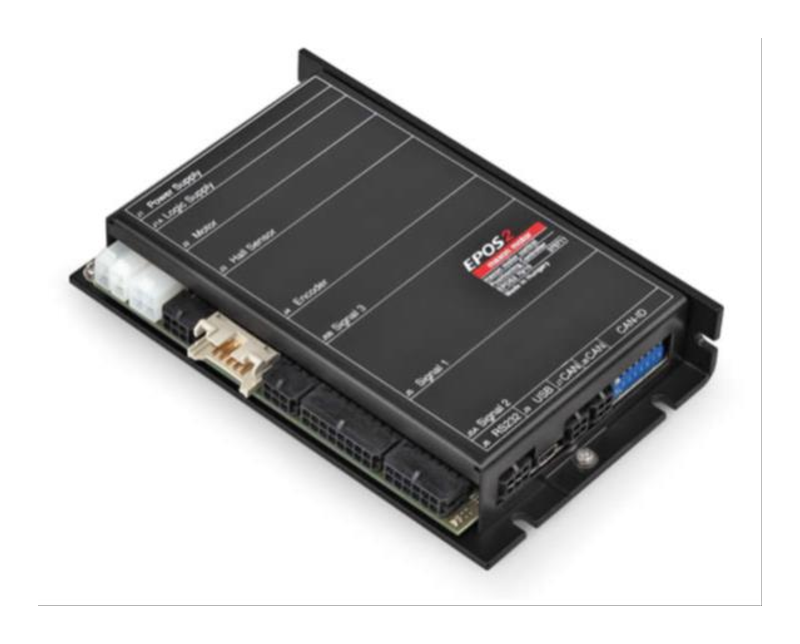
\includegraphics[angle=90,width=1\columnwidth]{figs/body02/FIGDEVICEDRIVEROPTION1.pdf}\\
  \caption[Controller driver (Option 1): Maxon Motor EPOS2 70/10 375711]{Controller driver (Option 1): Maxon Motor EPOS2 70/10 375711}
  \label{FIG:DEVICEDRIVEROPTION1}
\end{figure}
Maxon Motor EPOS2 70/10 375711 interfaces/pinouts can be seen in figure~\ref{FIG:DEVICEDRIVEROPTION1DRAWING}.
\begin{figure}
  \centering
  % Requires \usepackage{graphicx}
  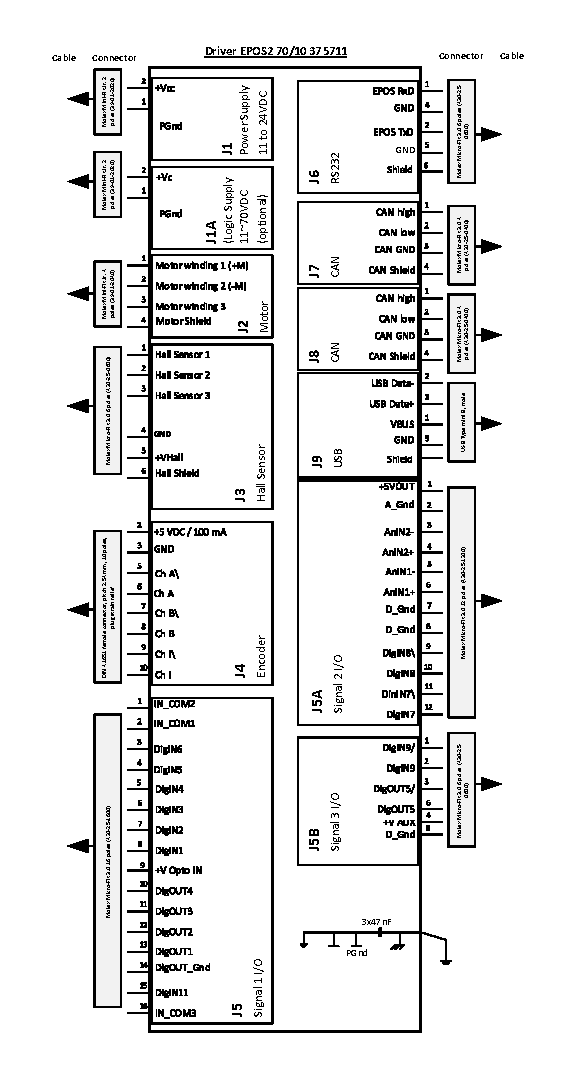
\includegraphics[angle=90,width=1\columnwidth]{figs/body02/FIGDEVICEDRIVEROPTION1DRAWING.pdf}\\
  \caption[Controller driver (Option 1): Maxon Motor EPOS2 70/10 375711 interfaces/pinout]{Controller driver (Option 1): Maxon Motor EPOS2 70/10 375711 interfaces/pinout}
  \label{FIG:DEVICEDRIVEROPTION1DRAWING}
\end{figure}
\subsection{Motor Combinations}
\subsubsection{1\textsuperscript{st} option: Maxon Motor Combination Part Number: 470625 - Items: Motor 305013 / Encoder 225778 / Reduction Gear 326660} \label{DEVICE:COMBINATION1}
\begin{itemize}
  \item Manufacturer: Maxon Motor
  \item Description:
  \begin{itemize}
    \item This motor combination was was specified by mechanics team (G1) with the aid guidelines of the electronics team (G2). This is an assembly of the motor 305013 (described in section~\ref{DEVICE:MOTOR1}), the encoder 225778 (described in section~\ref{DEVICE:ENCODER1}) and the reduction gear 326660 (described in section~\ref{DEVICE:GEAR1}) in a single combination. The gear is placed at the motor shaft output, and the encoder is placed at the motor base (see figure~\ref{FIG:DEVICECOMBINATIONOPTION1DRAWING}). Thus, the transmitted torque will always have passed through the gear reduction factor, but the encoder will be measuring the actual shaft speed (not considering the reduction).
  \end{itemize}
  \item Cable set:
  \begin{itemize}
    \item Encoder cable
    \item Hall effect sensor wires
    \item Motor supply wires
  \end{itemize}
  \item Documentation:
  \begin{itemize}
    \item Website: \href{http://www.maxonmotor.com/maxon/view/service\_search?query=470625}{http://www.maxonmotor.com/maxon/view/service\_search?query=470625}
    \item Datasheet: see website.
    \item Manual: see website.
    \item Sales contact: see G1 project.
  \end{itemize}
\end{itemize}
Maxon Motor Combination 470625 picture can be seen in figure~\ref{FIG:DEVICECOMBINATIONOPTION1}.
\begin{figure}
  \centering
  % Requires \usepackage{graphicx}
  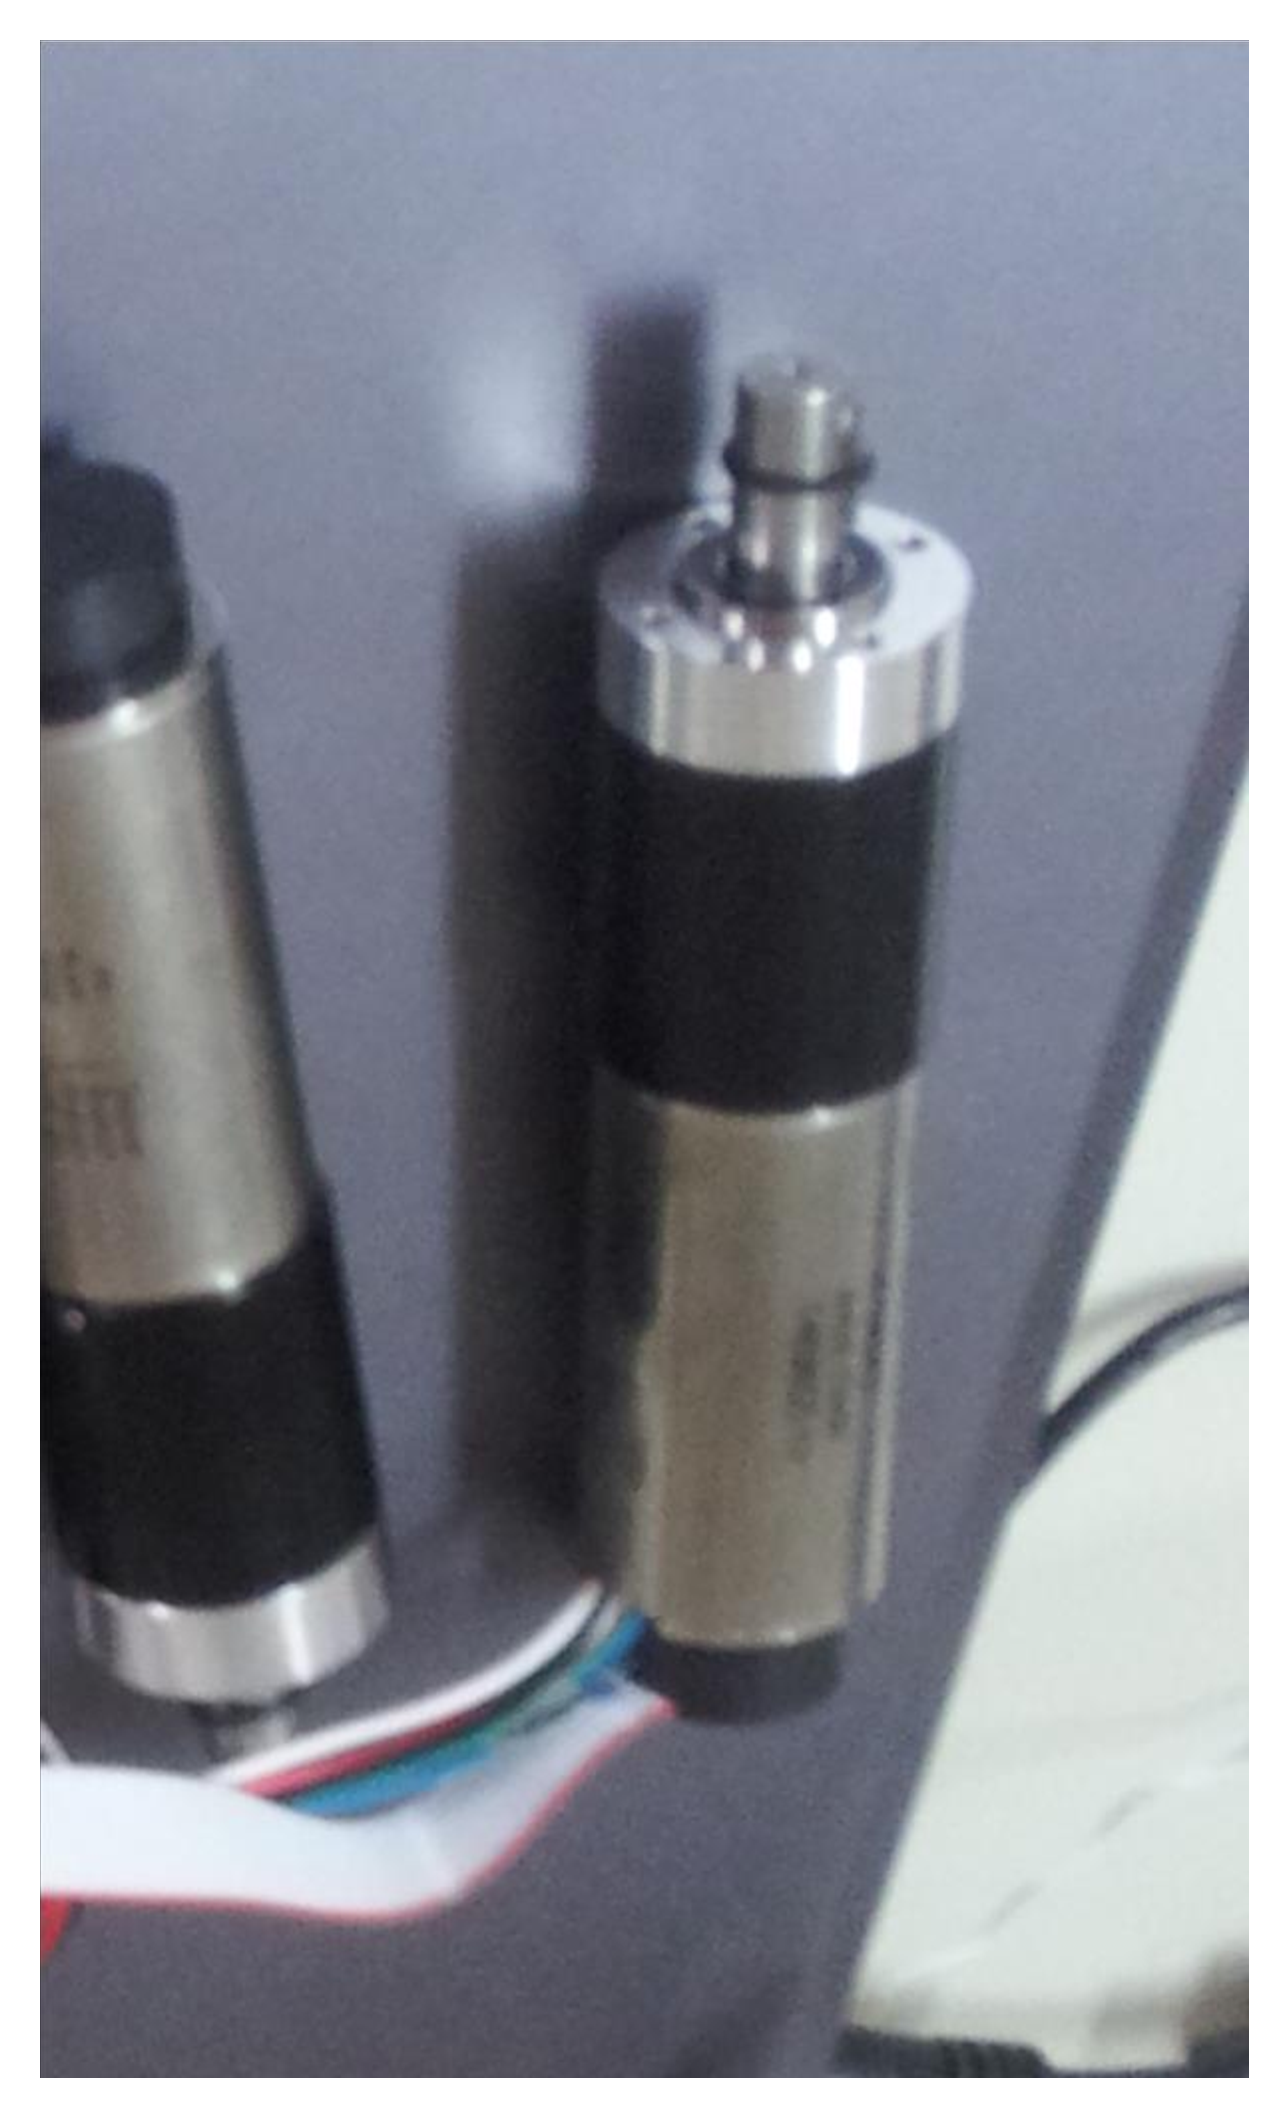
\includegraphics[angle=90,width=1\columnwidth]{figs/body02/FIGDEVICECOMBINATIONOPTION1.pdf}\\
  \caption[Motor combination (Option 1): Maxon Motor Combination 470625]{Motor combination (Option 1): Maxon Motor Combination 470625}
  \label{FIG:DEVICECOMBINATIONOPTION1}
\end{figure}
Maxon Motor EPOS2 70/10 375711 scheme and interfaces and can be seen in figure~\ref{FIG:DEVICECOMBINATIONOPTION1DRAWING}.
\begin{figure}
  \centering
  % Requires \usepackage{graphicx}
  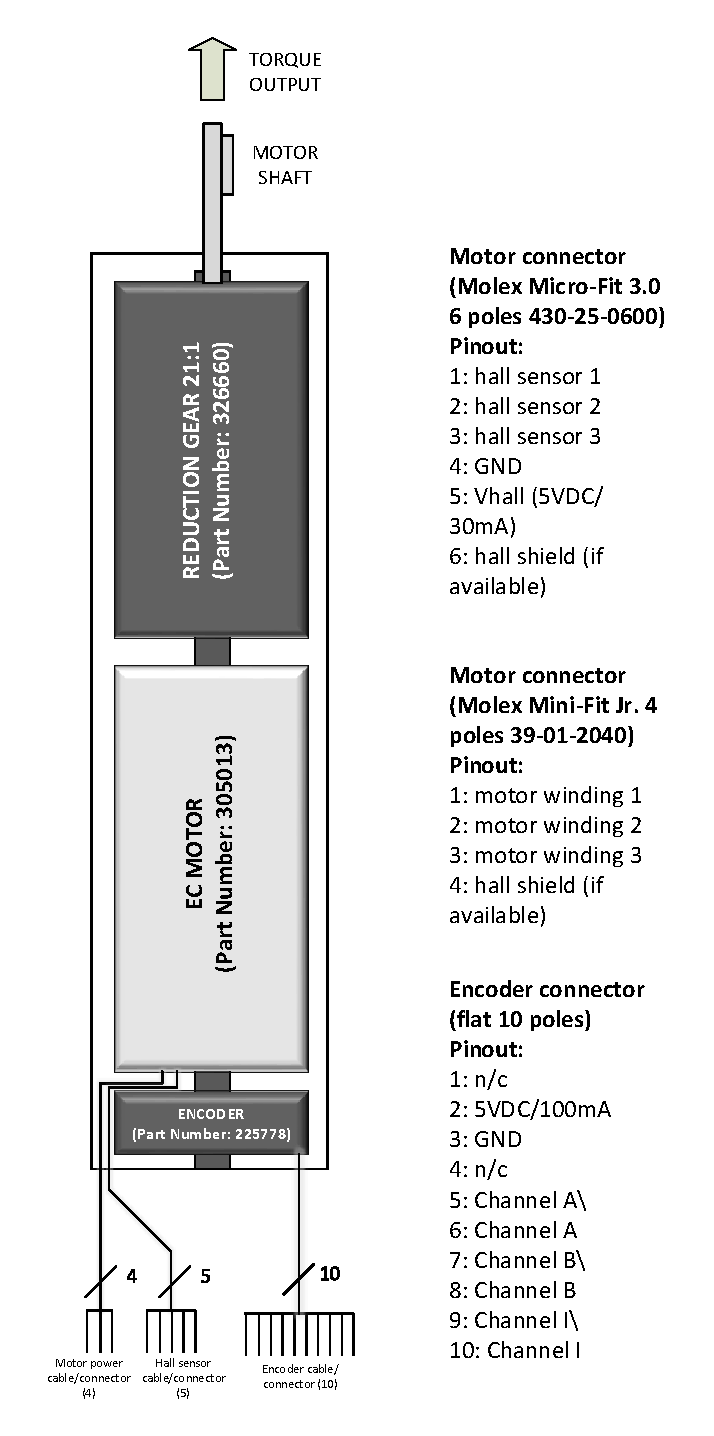
\includegraphics[angle=90,width=1\columnwidth]{figs/body02/FIGDEVICECOMBINATIONOPTION1DRAWING.pdf}\\
  \caption[Motor combination (Option 1): Maxon Motor Combination 470625 scheme and interfaces]{Motor combination (Option 1): Maxon Motor Combination 470625 scheme and interfaces}
  \label{FIG:DEVICECOMBINATIONOPTION1DRAWING}
\end{figure}
\section{Printed circuit boards}
\section{Electronic components}

\section{Wiring}
\subsection{Connectors} \label{DEVICE:CONNECTORS}
The following table (figure~\ref{FIG:DEVICECONNECTORTABLE1}) summarizes all the connectors that must be purchased for DORIS assembly. Each connector type has a respective connector acronym that appears in the cable list (section~\ref{DEVICE:CABLES}) as a easy reference for the cable connectors. In the next subsections, the most important connector types and pinouts are detailed. The possible commercial models for purchase are also suggested for each connector type.
\begin{figure}
  \centering
  % Requires \usepackage{graphicx}
  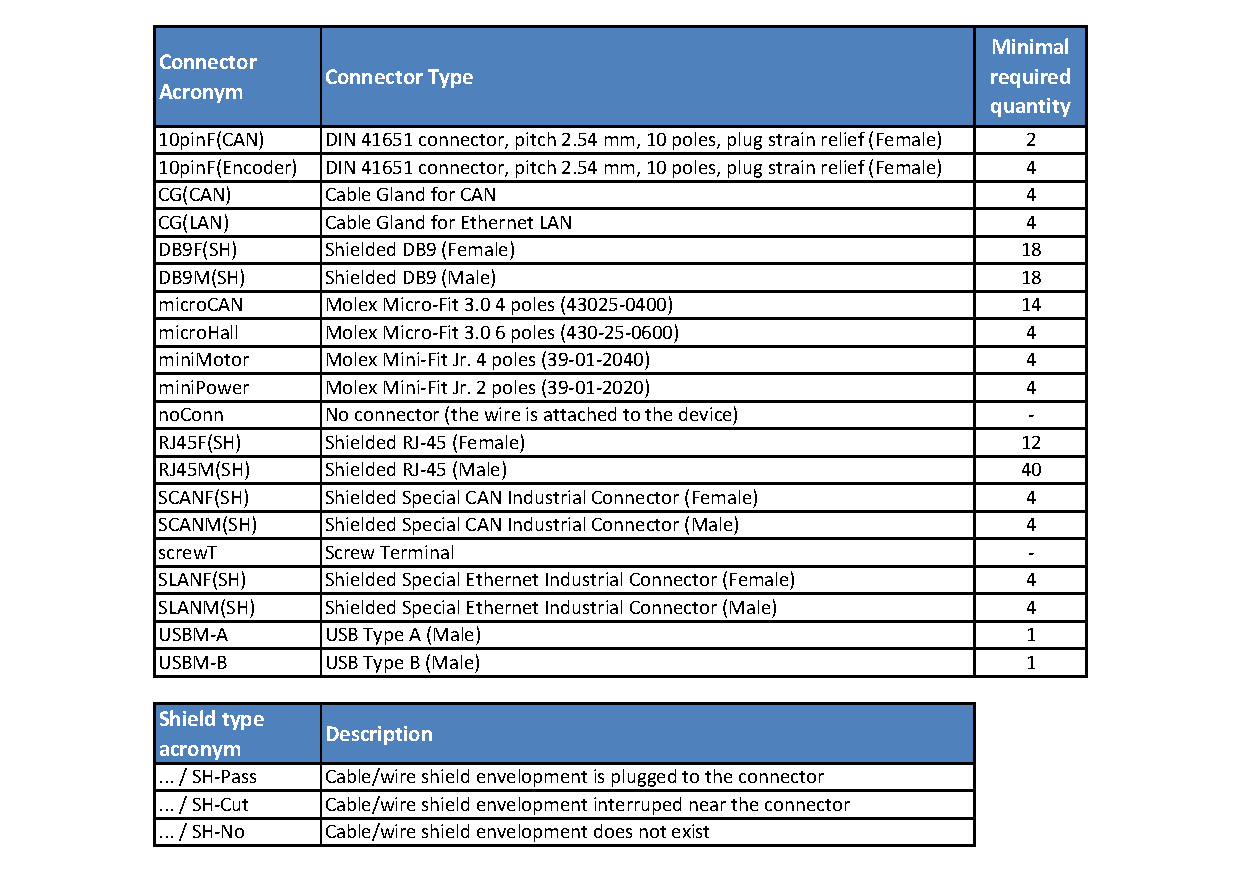
\includegraphics[angle=90,width=1\columnwidth]{figs/body02/FIGDEVICECONNECTORTABLE1.pdf}\\
  \caption[Connector table]{Connector table}
  \label{FIG:DEVICECONNECTORTABLE1}
\end{figure}
Also note that, for each cable connector at the "cable list", an acronym (SH-Pass, SH-Cut or SH-No) is designated. This indicates if the cable shield is plugged at the cable connector. The shield acronyms meanings are also described at the above connector table (figure~\ref{FIG:DEVICECONNECTORTABLE1}).

\subsubsection{10pinF(CAN): DIN 41651 connector, pitch 2.54 mm, 10 poles, plug strain relief (Female)} \label{DEVICE:10pinF(CAN)}
\begin{itemize}
  \item Acronym for cable/connector lists: 10pinF
  \item Name: DIN 41651 connector, pitch 2.54 mm, 10 poles, plug strain relief (Female)
  \item Picture and pinout: see figure~\ref{FIG:DEVICE10pinF(CAN)}
\end{itemize}
\begin{figure}
  \centering
  % Requires \usepackage{graphicx}
  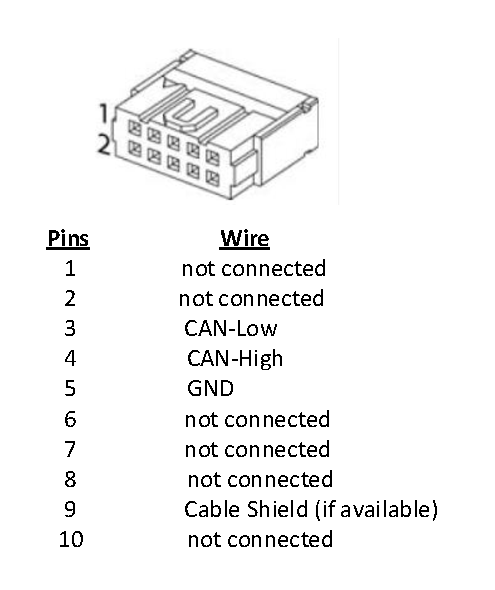
\includegraphics[angle=90,width=1\columnwidth]{figs/body02/FIGDEVICE10pinF(CAN).pdf}\\
  \caption[10pinF(CAN): DIN 41651 connector, pitch 2.54 mm, 10 poles, plug strain relief (Female)]{10pinF(CAN): DIN 41651 connector, pitch 2.54 mm, 10 poles, plug strain relief (Female)}
  \label{FIG:DEVICE10pinF(CAN)}
\end{figure}
\subsubsection{10pinF(Encoder): DIN 41651 connector, pitch 2.54 mm, 10 poles, plug strain relief (Female)} \label{DEVICE:10pinF(Encoder)}
\begin{itemize}
  \item Acronym for cable/connector lists: 10pinF(Encoder)
  \item Name: DIN 41651 connector, pitch 2.54 mm, 10 poles, plug strain relief (Female)
  \item Model references (Website): this connector type is provided together with the motor/driver combination package (described in sections~\ref{DEVICE:COMBINATION1} and~\ref{DEVICE:COMBINATION1}).
  \item Picture and pinout: see figure~\ref{FIG:DEVICE10pinF(Encoder)}
\end{itemize}
\begin{figure}
  \centering
  % Requires \usepackage{graphicx}
  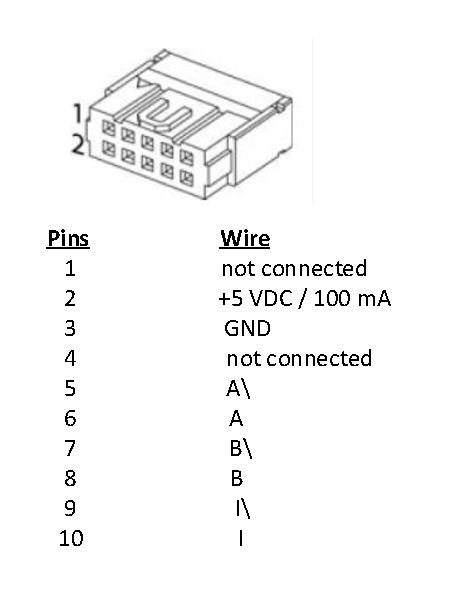
\includegraphics[angle=90,width=1\columnwidth]{figs/body02/FIGDEVICE10pinF(Encoder).pdf}\\
  \caption[10pinF(Encoder): DIN 41651 connector, pitch 2.54 mm, 10 poles, plug strain relief (Female)]{10pinF(Encoder): DIN 41651 connector, pitch 2.54 mm, 10 poles, plug strain relief (Female)}
  \label{FIG:DEVICE10pinF(Encoder)}
\end{figure}
\subsubsection{CG(CAN): Cable Gland for CAN} \label{DEVICE:CG(CAN)}
\begin{itemize}
  \item Acronym for cable/connector lists: CG(CAN)
  \item Name: Cable Gland for CAN
  \item Description: each CAN cable gland is used to fit one side of the outdoor CAN cable on the rear interface of each module. The presented option for this item can fit cables with 5mm to 10mm diameter, and is IP68 certified.
  \item Commercial option (Website): \href{http://www.digikey.com/product-detail/en/AIO-CSJM18/AIO-CSJM18-ND/3904970}{http://www.digikey.com/product-detail/en/AIO-CSJM18/AIO-CSJM18-ND/3904970}
  \item Picture and dimensions: see figure~\ref{DEVICE:CG(CAN)}
\end{itemize}
\begin{figure}
  \centering
  % Requires \usepackage{graphicx}
  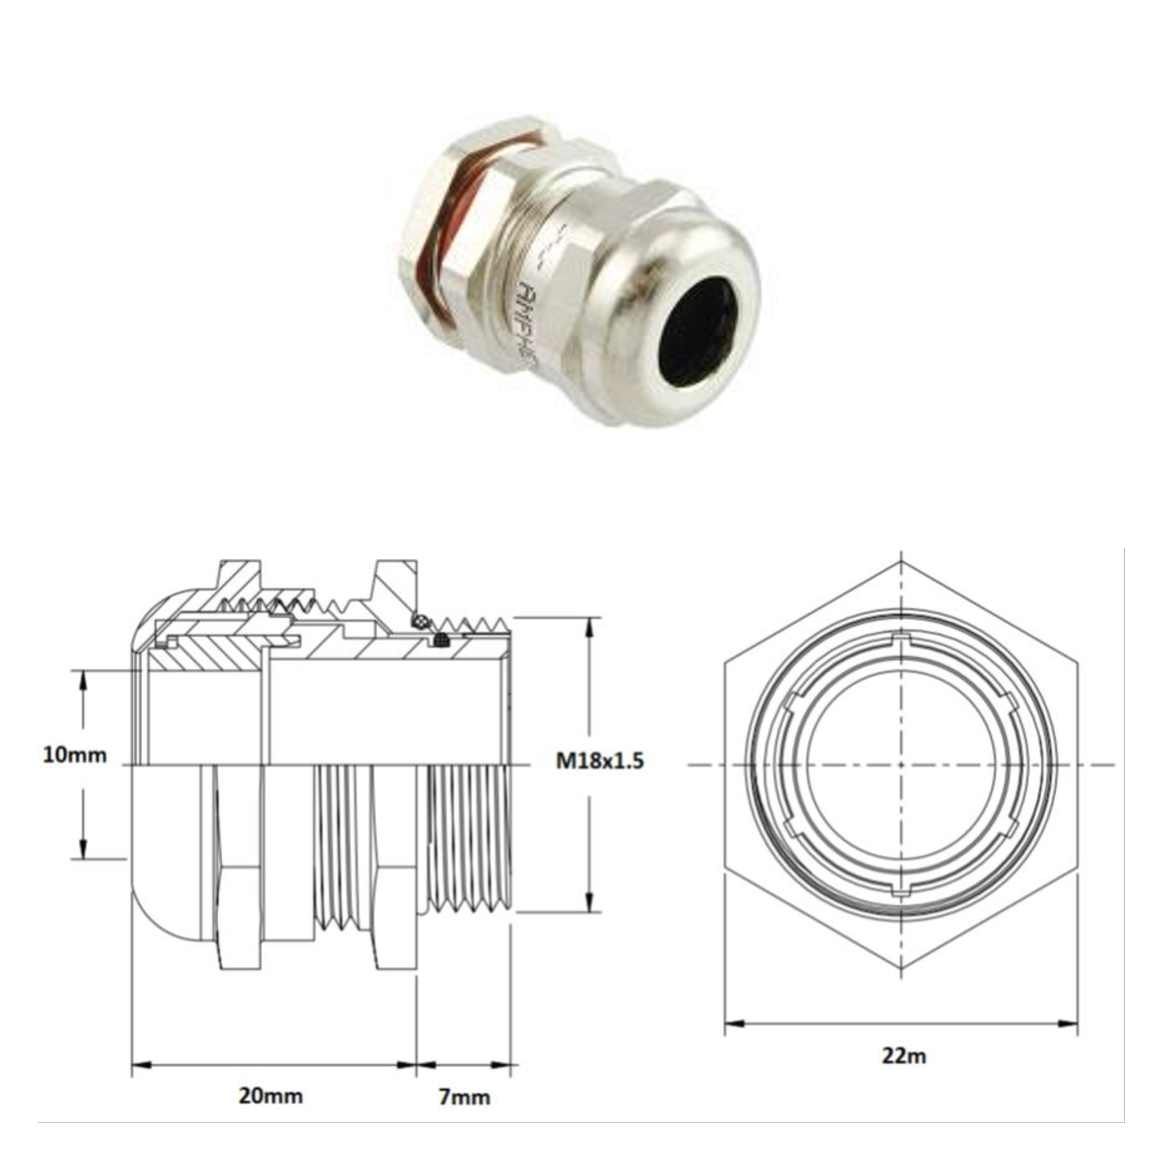
\includegraphics[angle=90,width=1\columnwidth]{figs/body02/FIGDEVICECG(CAN).pdf}\\
  \caption[CG(CAN): Cable Gland for CAN]{CG(CAN): Cable Gland for CAN}
  \label{FIG:DEVICE:CG(CAN)}
\end{figure}
\subsubsection{CG(LAN): Cable Gland for Ethernet LAN} \label{DEVICE:CG(LAN)}
\begin{itemize}
  \item Acronym for cable/connector lists: CG(LAN)
  \item Name: Cable Gland for Ethernet
  \item Description: each Ethernet cable gland is used to fit one side of the outdoor Ethernet cable on the rear interface of each module. The presented option for this item can fit cables with 5mm to 10mm diameter, and is IP68 certified.
  \item Commercial option (Website): \href{http://www.digikey.com/product-detail/en/AIO-CSJM18/AIO-CSJM18-ND/3904970}{http://www.digikey.com/product-detail/en/AIO-CSJM18/AIO-CSJM18-ND/3904970}
  \item Picture and dimensions: see figure~\ref{DEVICE:CG(LAN)}
\end{itemize}
\begin{figure}
  \centering
  % Requires \usepackage{graphicx}
  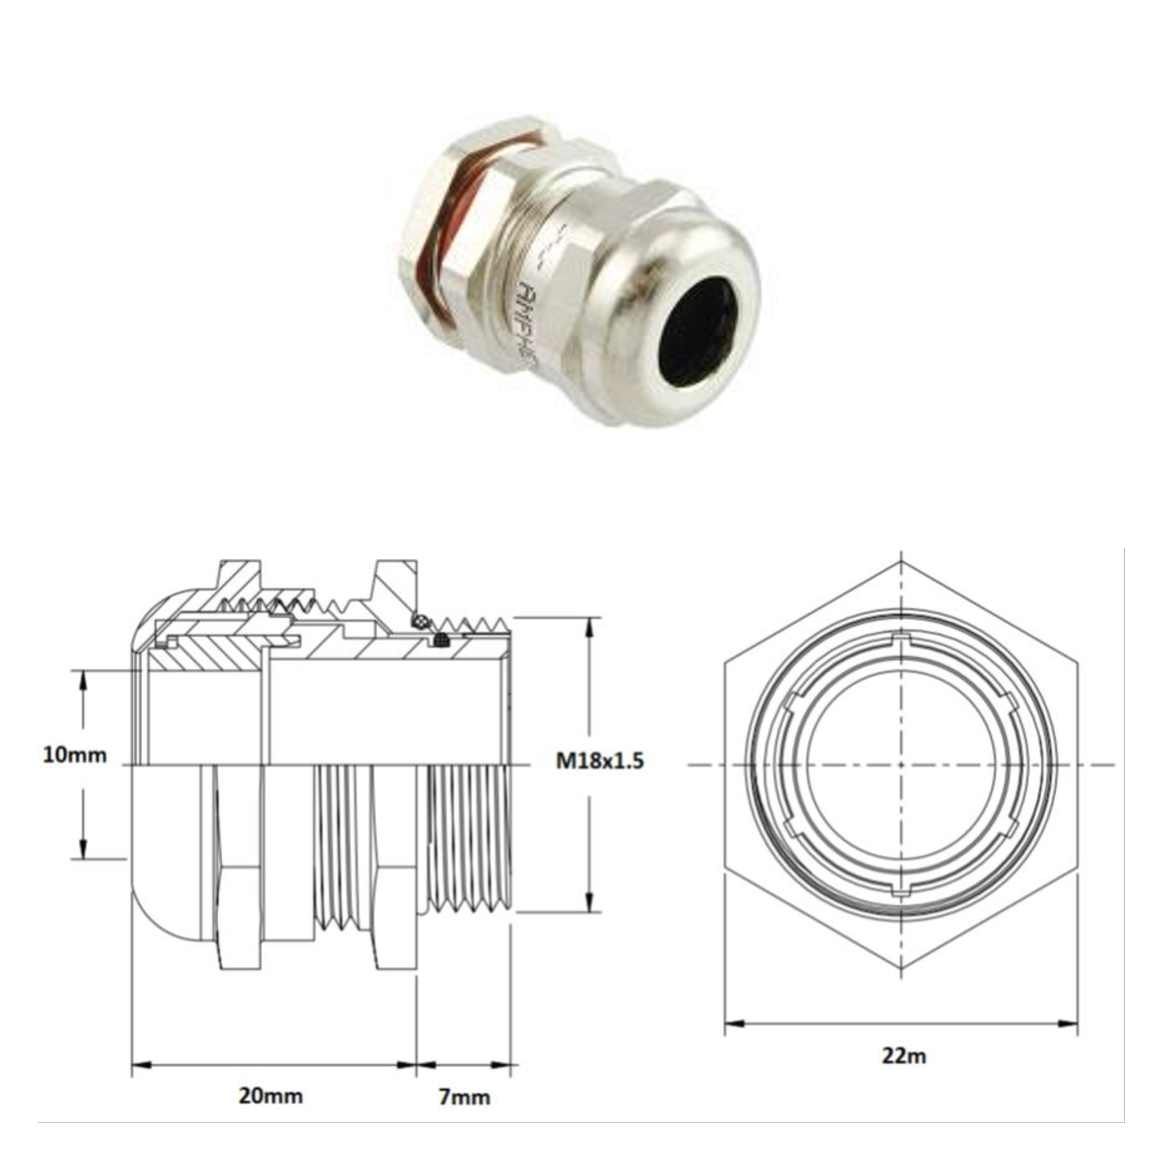
\includegraphics[angle=90,width=1\columnwidth]{figs/body02/FIGDEVICECG(LAN).pdf}\\
  \caption[CG(LAN): Cable Gland for Ethernet]{CG(LAN): Cable Gland for Ethernet}
  \label{FIG:DEVICE:CG(LAN)}
\end{figure}
\subsubsection{DB9F(SH): Shielded DB9 (Female)} \label{DEVICE:DB9F(SH)}
\begin{itemize}
  \item Acronym for cable/connector lists: DB9F(SH)
  \item Name: Shielded DB9 (Female)
  \item Commercial option (Website): \href{http://www.digikey.com/product-detail/en/D09S13A4GL00LF/609-1482-ND/1001796}{http://www.digikey.com/product-detail/en/D09S13A4GL00LF/609-1482-ND/1001796}
  \item Picture and pinout: see figure~\ref{FIG:DEVICEDB9F(SH)}
\end{itemize}
\begin{figure}
  \centering
  % Requires \usepackage{graphicx}
  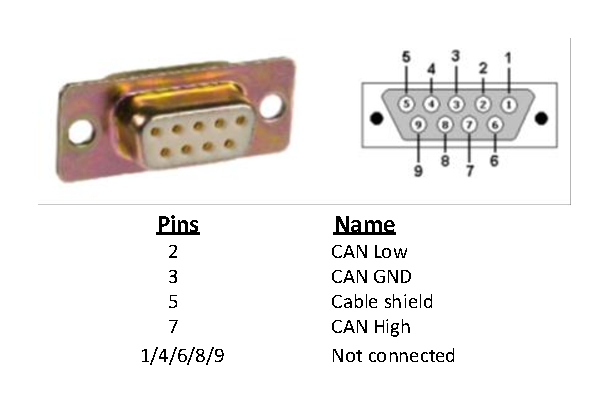
\includegraphics[angle=90,width=1\columnwidth]{figs/body02/FIGDEVICEDB9F(SH).pdf}\\
  \caption[DB9F(SH): Shielded DB9 (Female)]{DB9F(SH): Shielded DB9 (Female)}
  \label{FIG:DEVICEDB9F(SH)}
\end{figure}
\subsubsection{DB9M(SH): Shielded DB9 (Male)} \label{DEVICE:DB9M(SH)}
\begin{itemize}
  \item Acronym for cable/connector lists: DB9M(SH)
  \item Name: Shielded DB9 (Male)
  \item Commercial option (Website): \href{http://www.digikey.com/product-detail/en/DE09P064TXLF/609-1524-ND/1001838}{http://www.digikey.com/product-detail/en/DE09P064TXLF/609-1524-ND/1001838}
  \item Picture and pinout: see figure~\ref{FIG:DEVICEDB9M(SH)}
\end{itemize}
\begin{figure}
  \centering
  % Requires \usepackage{graphicx}
  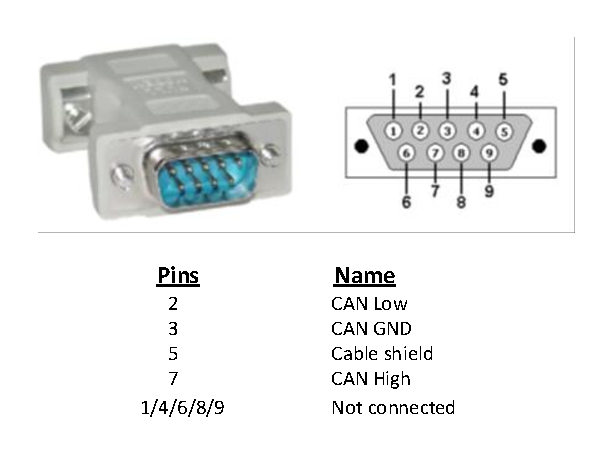
\includegraphics[angle=90,width=1\columnwidth]{figs/body02/FIGDEVICEDB9M(SH).pdf}\\
  \caption[DB9M(SH): Shielded DB9 (Male)]{DB9M(SH): Shielded DB9 (Male)}
  \label{FIG:DEVICEDB9M(SH)}
\end{figure}
\subsubsection{microCAN: Molex Micro-Fit 3.0\texttrademark 4 poles (43025-0400)} \label{DEVICE:microCAN}
\begin{itemize}
  \item Acronym for cable/connector lists: microCAN
  \item Name: Molex Micro-Fit 3.0\texttrademark 4 poles, Part Number: 43025-0400
  \item Model references (Website): \href{http://www.molex.com/molex/products/datasheet.jsp?part=active/0430250400\_CRIMP\_HOUSINGS.xml}{http://www.molex.com/molex/products/datasheet.jsp?part=active/0430250400\_CRIMP\_HOUSINGS.xml}
  \item Picture and pinout: see figure~\ref{FIG:DEVICEmicroCAN}
  \item Commercial option (Website): \href{http://www.digikey.com/product-search/en?WT.z\_header=search\_go\&lang=en\&site=us\&keywords=43025-0400\&x=0\&y=0\&formaction=on}{http://www.digikey.com/product-search/en?WT.z\_header=search\_go\&lang=en\&site=us\&keywords=43025-0400\&x=0\&y=0\&formaction=on}
\end{itemize}
\begin{figure}
  \centering
  % Requires \usepackage{graphicx}
  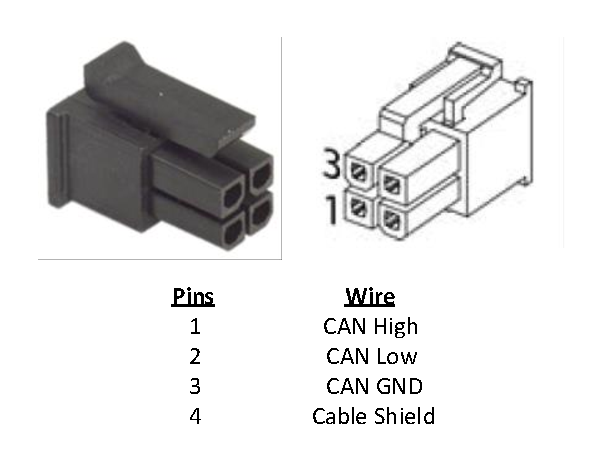
\includegraphics[angle=90,width=1\columnwidth]{figs/body02/FIGDEVICEmicroCAN.pdf}\\
  \caption[microCAN: Molex Micro-Fit 3.0\texttrademark 4 poles (43025-0400)]{microCAN: Molex Micro-Fit 3.0\texttrademark 4 poles (43025-0400)}
  \label{FIG:DEVICEmicroCAN}
\end{figure}

\subsubsection{microHall: Molex Micro-Fit 3.0\texttrademark 6 poles (43025-0600)} \label{DEVICE:microHall}
\begin{itemize}
  \item Acronym for cable/connector lists: microHall
  \item Name: Molex Micro-Fit 3.0\texttrademark 6 poles, Part Number: 43025-0600
  \item Model references (Website): \href{http://www.molex.com/molex/products/datasheet.jsp?part=active/0430250600\_CRIMP\_HOUSINGS.xml}{http://www.molex.com/molex/products/datasheet.jsp?part=active/0430250600\_CRIMP\_HOUSINGS.xml}
  \item Commercial option (Website): \href{http://www.digikey.com/product-search/en?WT.z\_header=search\_go\&lang=en\&site=us\&keywords=43025-0600\&x=0\&y=0\&formaction=on}{http://www.digikey.com/product-search/en?WT.z\_header=search\_go\&lang=en\&site=us\&keywords=43025-0600\&x=0\&y=0\&formaction=on}
  \item Picture and pinout: see figure~\ref{FIG:DEVICEmicroHall}
\end{itemize}
\begin{figure}
  \centering
  % Requires \usepackage{graphicx}
  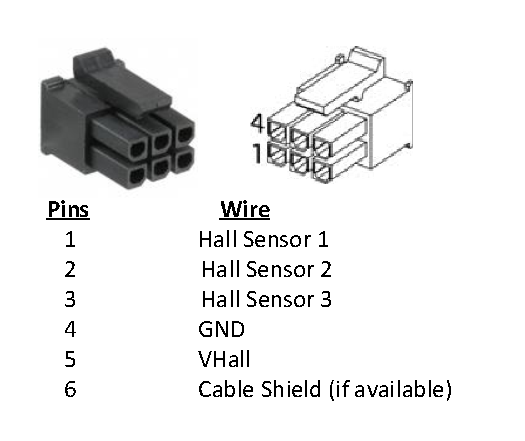
\includegraphics[angle=90,width=1\columnwidth]{figs/body02/FIGDEVICEmicroHall.pdf}\\
  \caption[microHall: Molex Micro-Fit 3.0\texttrademark 6 poles (43025-0600)]{microHall: Molex Micro-Fit 3.0\texttrademark 6 poles (43025-0600)}
  \label{FIG:DEVICEmicroHall}
\end{figure}
\subsubsection{miniMotor: Molex Mini-Fit\textregistered Jr. 4 poles (39-01-2040)} \label{DEVICE:miniMotor}
\begin{itemize}
  \item Acronym for cable/connector lists: miniMotor
  \item Name: Molex Mini-Fit\textregistered Jr. 4 poles, Part Number: 39-01-2040
  \item Model references (Website): \href{http://www.molex.com/molex/products/datasheet.jsp?part=active/0039012040\_CRIMP\_HOUSINGS.xml}{http://www.molex.com/molex/products/datasheet.jsp?part=active/0039012040\_CRIMP\_HOUSINGS.xml}
  \item Commercial option (Website): \href{http://www.digikey.com/product-search/en?vendor=0\&keywords=39-01-2040}{http://www.digikey.com/product-search/en?vendor=0\&keywords=39-01-2040}
  \item Picture and pinout: see figure~\ref{FIG:DEVICEminiMotor}
\end{itemize}
\begin{figure}
  \centering
  % Requires \usepackage{graphicx}
  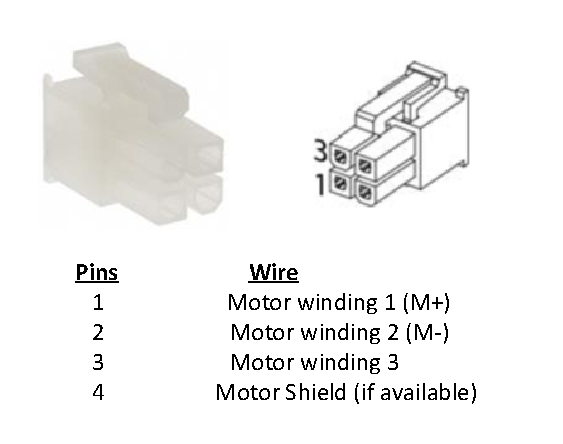
\includegraphics[angle=90,width=1\columnwidth]{figs/body02/FIGDEVICEminiMotor.pdf}\\
  \caption[miniMotor: Molex Mini-Fit\textregistered Jr. 4 poles (39-01-2040)]{miniMotor: Molex Mini-Fit\textregistered Jr. 4 poles (39-01-2040)}
  \label{FIG:DEVICEminiMotor}
\end{figure}
\subsubsection{miniPower: Molex Mini-Fit\textregistered Jr. 2 poles (39-01-2020)} \label{DEVICE:miniPower}
\begin{itemize}
  \item Acronym for cable/connector lists: miniPower
  \item Name: Molex Mini-Fit\textregistered Jr. 2 poles, Part Number: 39-01-2020
  \item Model references (Website): \href{http://www.molex.com/molex/products/datasheet.jsp?part=active/0039012020\_CRIMP\_HOUSINGS.xml}{http://www.molex.com/molex/products/datasheet.jsp?part=active/0039012020\_CRIMP\_HOUSINGS.xml}
  \item Commercial option (Website): \href{http://www.digikey.com/product-search/en?WT.z\_header=search\_go\&lang=en\&site=us\&keywords=39-01-2020\&x=0\&y=0\&formaction=on}{http://www.digikey.com/product-search/en?WT.z\_header=search\_go\&lang=en\&site=us\&keywords=39-01-2020\&x=0\&y=0\&formaction=on}
  \item Picture and pinout: see figure~\ref{FIG:DEVICEminiPower}
\end{itemize}
\begin{figure}
  \centering
  % Requires \usepackage{graphicx}
  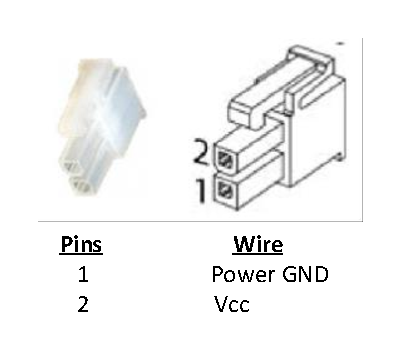
\includegraphics[angle=90,width=1\columnwidth]{figs/body02/FIGDEVICEminiPower.pdf}\\
  \caption[miniPower: Molex Mini-Fit\textregistered Jr. 2 poles (39-01-2020)]{miniPower: Molex Mini-Fit\textregistered Jr. 2 poles (39-01-2020)}
  \label{FIG:DEVICEminiPower}
\end{figure}
\subsubsection{RJ45F(SH): Shielded RJ-45 (Female)} \label{DEVICE:RJ45F(SH)}
\begin{itemize}
  \item Acronym for cable/connector lists: RJ45F(SH)
  \item Name: Shielded RJ-45 (Female)
  \item Model references (Website): ESCREVER
  \item Picture and pinout: see figure~\ref{FIG:DEVICERJ45F(SH)}
\end{itemize}
\begin{figure}
  \centering
  % Requires \usepackage{graphicx}
  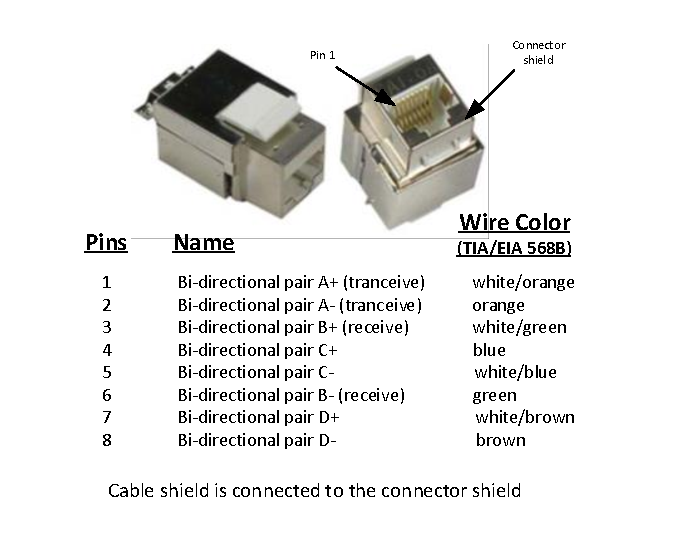
\includegraphics[angle=90,width=1\columnwidth]{figs/body02/FIGDEVICERJ45F(SH).pdf}\\
  \caption[RJ45F(SH): Shielded RJ-45 (Female)]{RJ45F(SH): Shielded RJ-45 (Female)}
  \label{FIG:DEVICERJ45F(SH)}
\end{figure}
\subsubsection{RJ45M(SH): Shielded RJ-45 (Male)} \label{DEVICE:RJ45M(SH)}
\begin{itemize}
  \item Acronym for cable/connector lists: RJ45M(SH)
  \item Name: Shielded RJ-45 (Male)
  \item Model references (Website): ESCREVER
  \item Picture and pinout: see figure~\ref{FIG:DEVICERJ45M(SH)}
\end{itemize}
\begin{figure}
  \centering
  % Requires \usepackage{graphicx}
  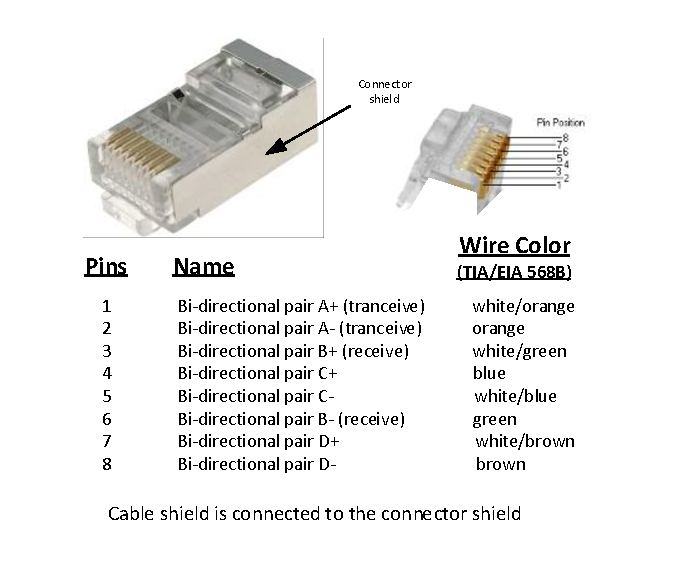
\includegraphics[angle=90,width=1\columnwidth]{figs/body02/FIGDEVICERJ45M(SH).pdf}\\
  \caption[RJ45M(SH): Shielded RJ-45 (Male)]{RJ45M(SH): Shielded RJ-45 (Male)}
  \label{FIG:DEVICERJ45M(SH)}
\end{figure}
\subsubsection{SCANF(SH): Shielded Special CAN Industrial Connector (Female)} \label{DEVICE:SCANF(SH)}
\begin{itemize}
  \item Acronym for cable/connector lists: SCANF(SH)
  \item Name: Shielded Special CAN Industrial Connector (Female)
  \item Description: This connector type is used for the CAN cables that are used outside DORIS modules. Hence, its protection level is higher. The presented option for this connector is a 4 position M12 (Female) with IP67 certification.
  \item Commercial option (Website): \href{http://www.digikey.com/product-detail/en/1838274-2/A97641-ND/1764156}{http://www.digikey.com/product-detail/en/1838274-2/A97641-ND/1764156}
  \item Picture and pinout: see figure~\ref{FIG:DEVICESCANF(SH)}
\end{itemize}
\begin{figure}
  \centering
  % Requires \usepackage{graphicx}
  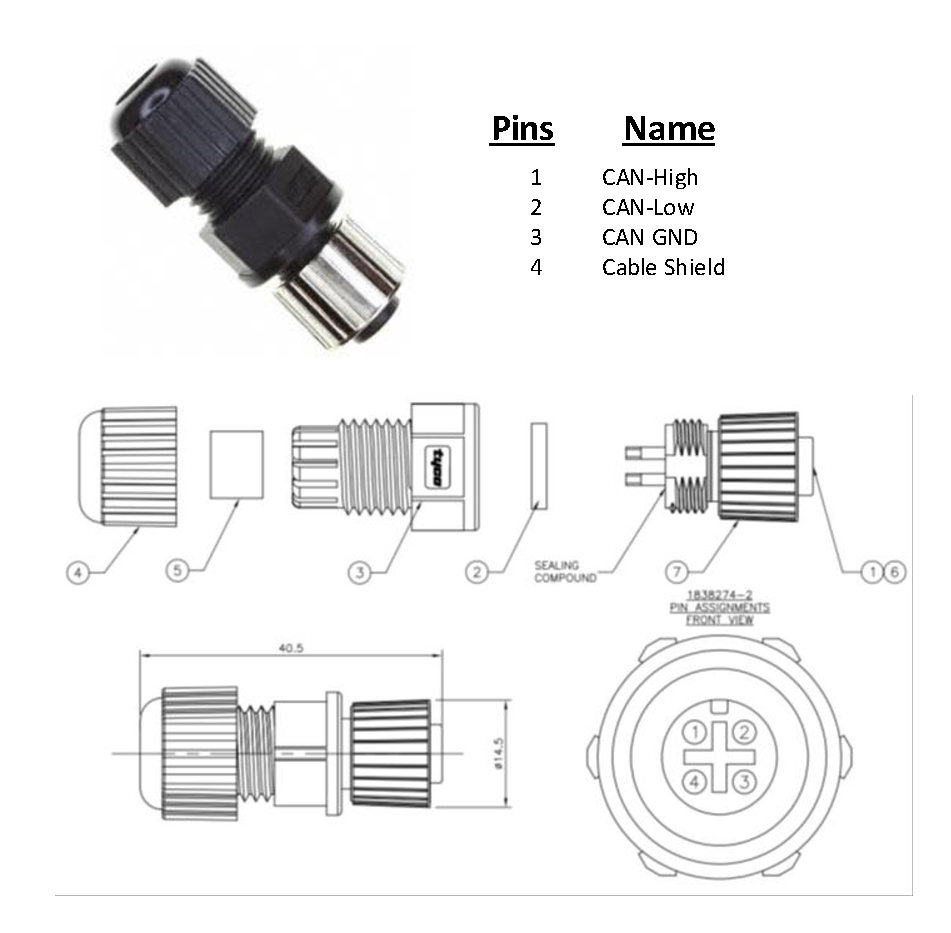
\includegraphics[angle=90,width=1\columnwidth]{figs/body02/FIGDEVICESCANF(SH).pdf}\\
  \caption[SCANF(SH): Shielded Special CAN Industrial Connector (Female)]{SCANF(SH): Shielded Special CAN Industrial Connector (Female)}
  \label{FIG:DEVICESCANF(SH)}
\end{figure}
\subsubsection{SCANM(SH): Shielded Special CAN Industrial Connector (Male)} \label{DEVICE:SCANM(SH)}
\begin{itemize}
  \item Acronym for cable/connector lists: SCANM(SH)
  \item Name: Shielded Special CAN Industrial Connector (Male)
  \item Description: This connector type is used for the CAN cables that are used outside DORIS modules. Hence, its protection level is higher. The presented option for this connector is a 4 position M12 (Male) with IP67 certification.
  \item Commercial option (Website): \href{http://www.digikey.com/product-detail/en/1838277-2/A97670-ND/1764185}{http://www.digikey.com/product-detail/en/1838277-2/A97670-ND/1764185}
  \item Picture and pinout: see figure~\ref{FIG:DEVICESCANM(SH)}
\end{itemize}
\begin{figure}
  \centering
  % Requires \usepackage{graphicx}
  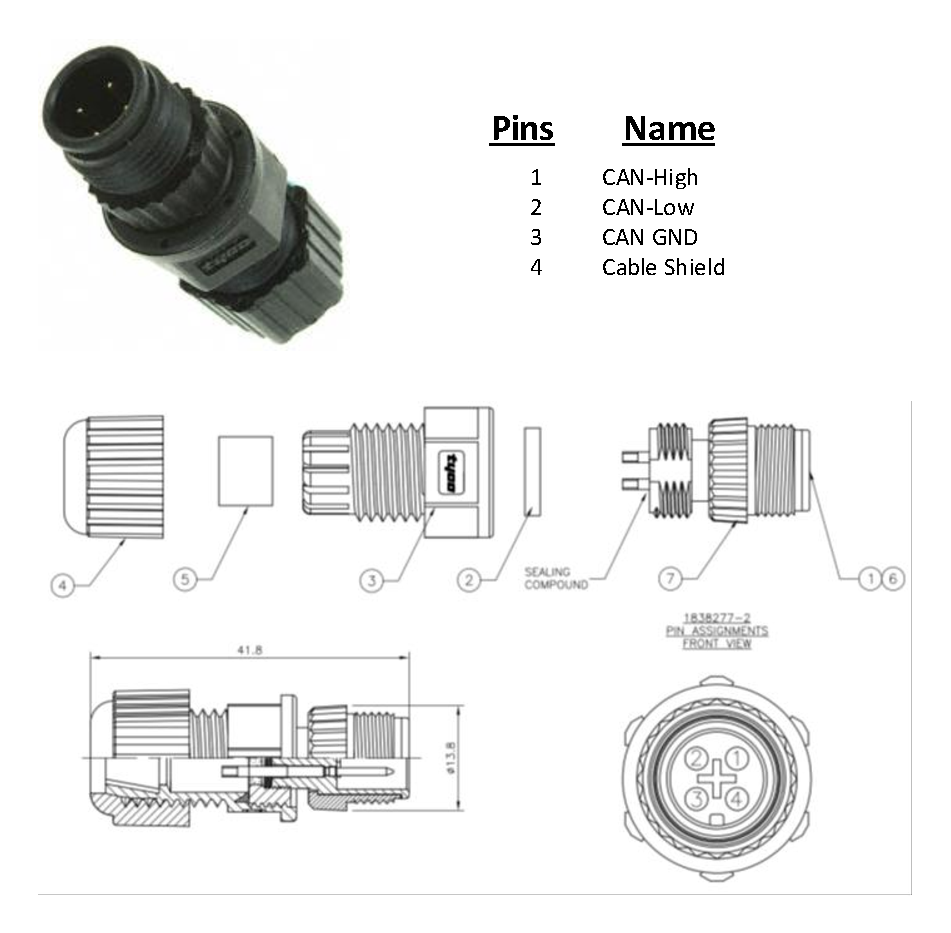
\includegraphics[angle=90,width=1\columnwidth]{figs/body02/FIGDEVICESCANM(SH).pdf}\\
  \caption[SCANM(SH): Shielded Special CAN Industrial Connector (Male)]{SCANM(SH): Shielded Special CAN Industrial Connector (Male)}
  \label{FIG:DEVICESCANM(SH)}
\end{figure}
\subsubsection{SLANF(SH): Shielded Special Ethernet Industrial Connector (Female)} \label{DEVICE:SLANF(SH)}
\begin{itemize}
  \item Acronym for cable/connector lists: SLANF(SH)
  \item Name: Shielded Special Ethernet Industrial Connector (Female)
  \item Description: This connector type is used for the Ethernet cables that are used outside DORIS modules. Hence, its protection level is higher. The presented option for this connector is a RJ-45 (Female) with IP67 certification.
  \item Commercial option (Website): \href{http://www.digikey.com/product-search/en?v=626\&mpart=17-10017}{http://www.digikey.com/product-search/en?v=626\&mpart=17-10017}
  \item Picture and pinout: see figure~\ref{FIG:DEVICESLANF(SH)}
\end{itemize}
\begin{figure}
  \centering
  % Requires \usepackage{graphicx}
  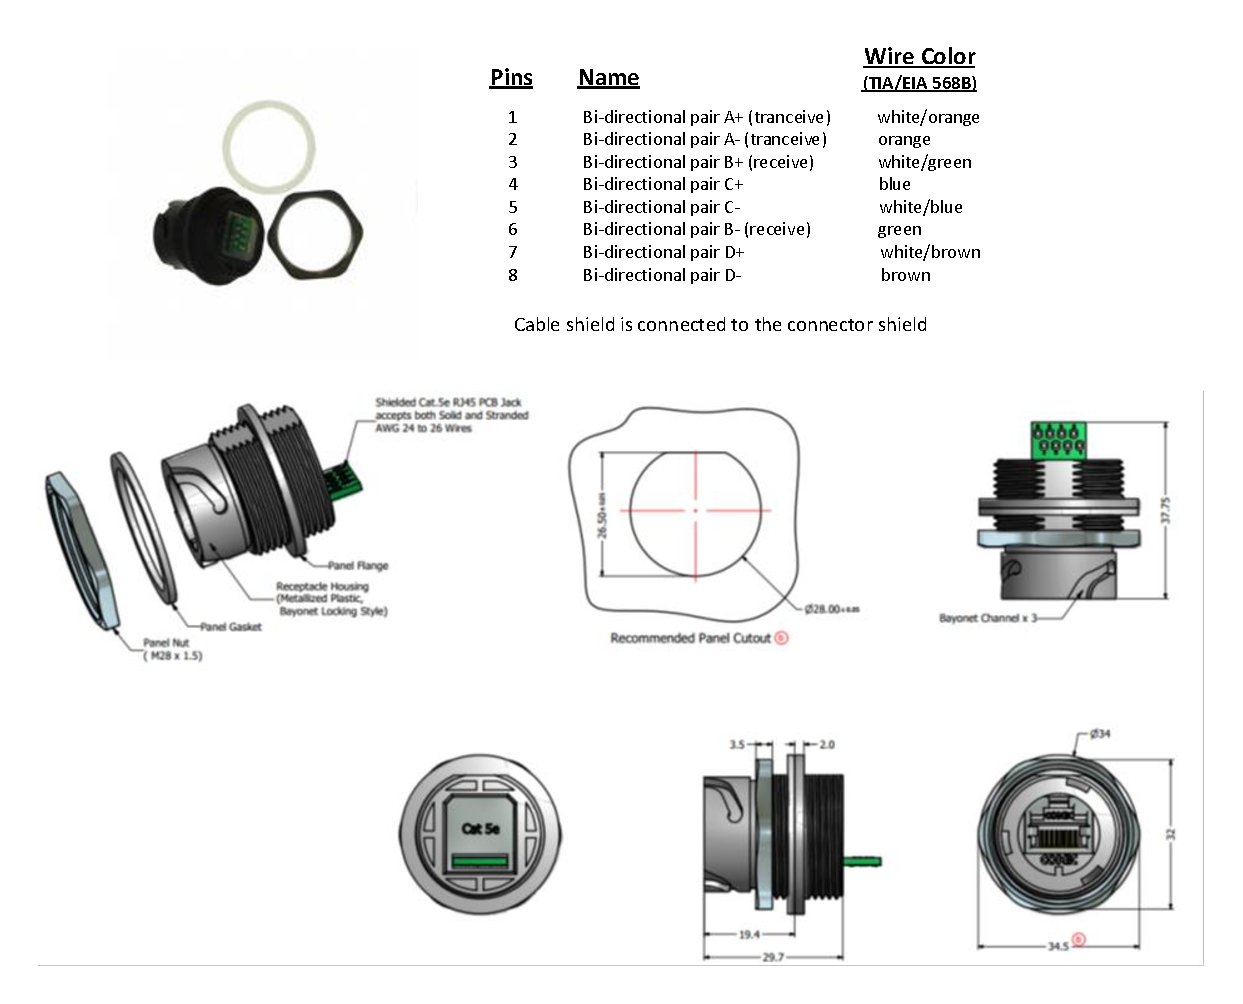
\includegraphics[angle=90,width=1\columnwidth]{figs/body02/FIGDEVICESLANF(SH).pdf}\\
  \caption[SLANF(SH): Shielded Special Ethernet Industrial Connector (Female)]{SLANF(SH): Shielded Special Ethernet Industrial Connector (Female)}
  \label{FIG:DEVICESLANF(SH)}
\end{figure}
\subsubsection{SLANM(SH): Shielded Special Ethernet Industrial Connector (Male)} \label{DEVICE:SLANM(SH)}
\begin{itemize}
  \item Acronym for cable/connector lists: SLANM(SH)
  \item Name: Shielded Special Ethernet Industrial Connector (Male)
  \item Description: This connector type is used for the Ethernet cables that are used outside DORIS modules. Hence, its protection level is higher. The presented option for this connector is a RJ-45 (Male) with IP67 certification and a cable gland.
  \item Commercial option (Website): \href{http://www.digikey.com/product-detail/en/17-10001/626-1294-ND/1618640}{http://www.digikey.com/product-detail/en/17-10001/626-1294-ND/1618640}
  \item Picture and pinout: see figure~\ref{FIG:DEVICESLANM(SH)}
\end{itemize}
\begin{figure}
  \centering
  % Requires \usepackage{graphicx}
  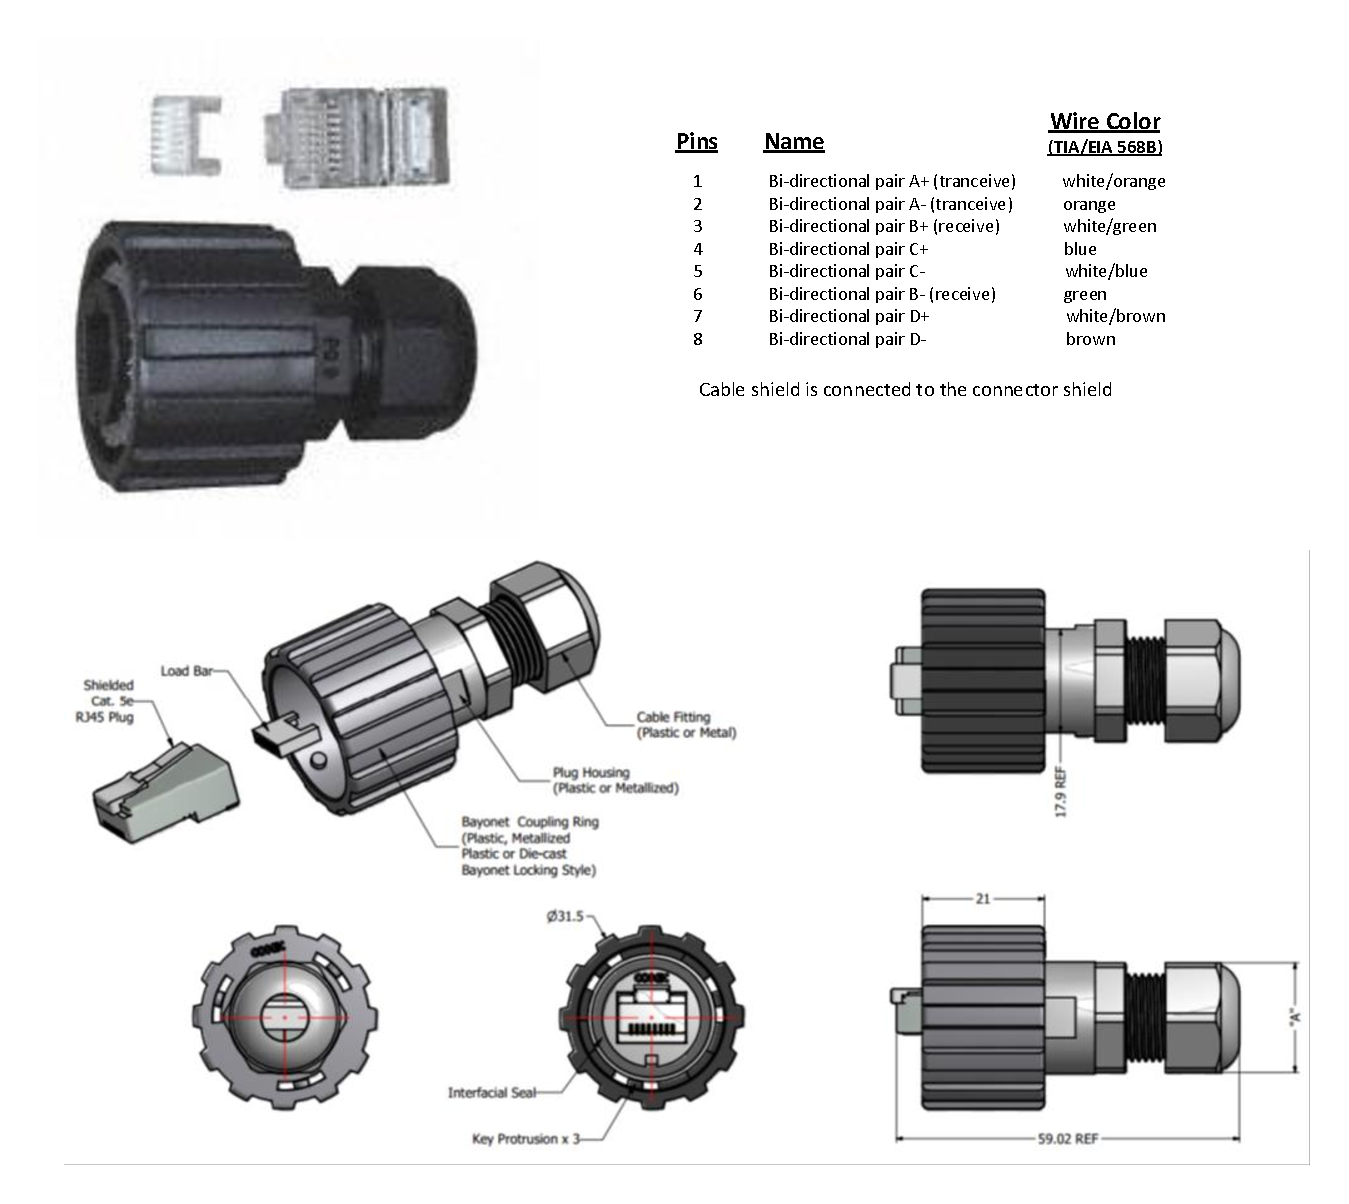
\includegraphics[angle=90,width=1\columnwidth]{figs/body02/FIGDEVICESLANM(SH).pdf}\\
  \caption[SLANM(SH): Shielded Special Ethernet Industrial Connector (Male)]{SLANM(SH): Shielded Special Ethernet Industrial Connector (Male)}
  \label{FIG:DEVICESLANM(SH)}
\end{figure}
\subsection{Cables} \label{DEVICE:CABLES}
ESCREVER
The table (figure~\ref{FIG:CABLELIST}) summarizes all the communication cables that must be prepared for DORIS assembly. For each cable, you must check at the cable list:
\begin{itemize}
  \item Cable tag:
  \begin{itemize}
    \item For each communication cable, a tag is assigned in order to facilitate its identification. The cable tagging follows the standard described in figure~\ref{FIG:CABLETAGGING}.
    \item Each cable must be physically identified with a cable mark showing its tag. It is recommended the use of ovalgrips, as shown in figure~\ref{FIG:OVALGRIP}.
  \end{itemize}
  \item Connectors:
  \begin{itemize}
    \item At the cable list, the connectors at both origin and destination are defined by an acronym. Check the acronyms at the connector section (section~\ref{DEVICE:CONNECTORS}) and at the connector table (figure~\ref{FIG:DEVICECONNECTORTABLE1}) to understand the specifications of each connector type, such as: pinout, commercial model, IP protection, shield.
    \item Also check at the connector table (figure~\ref{FIG:DEVICECONNECTORTABLE1}) if the cable shield (if present) must pass through the connector or if it must be interrupted near the connector.
  \end{itemize}
  \item Cable signal type:
  \begin{itemize}
    \item Each cable is used for a different purpose. For each purpose, a different cable type is required. The cable type list is presented in figure~\ref{FIG:CABLETYPELIST}.
  \end{itemize}
  \item Construction type:
  \begin{itemize}
    \item Each cable has a different way to be constructed. Construction types are distinguished by:
    \begin{itemize}
      \item Commercial cable model to be used.
      \item Connector types to be used.
      \item Presence (or not) of shield envelopment.
      \item Shield passage, i.e., if the shield envelopment or wire passes through the connector or not.
    \end{itemize}
    \item Each construction type is defined by an acronym.
    \item Details of each construction type can be found at the section~\ref{CONSTRUCTIONS}.
  \end{itemize}
  \item Length:
  \begin{itemize}
    \item The lengths defined in the cable list are estimated values. Updates may occur in future revisions of this memorandum.
  \end{itemize}
\end{itemize}
\begin{figure}
  \centering
  % Requires \usepackage{graphicx}
  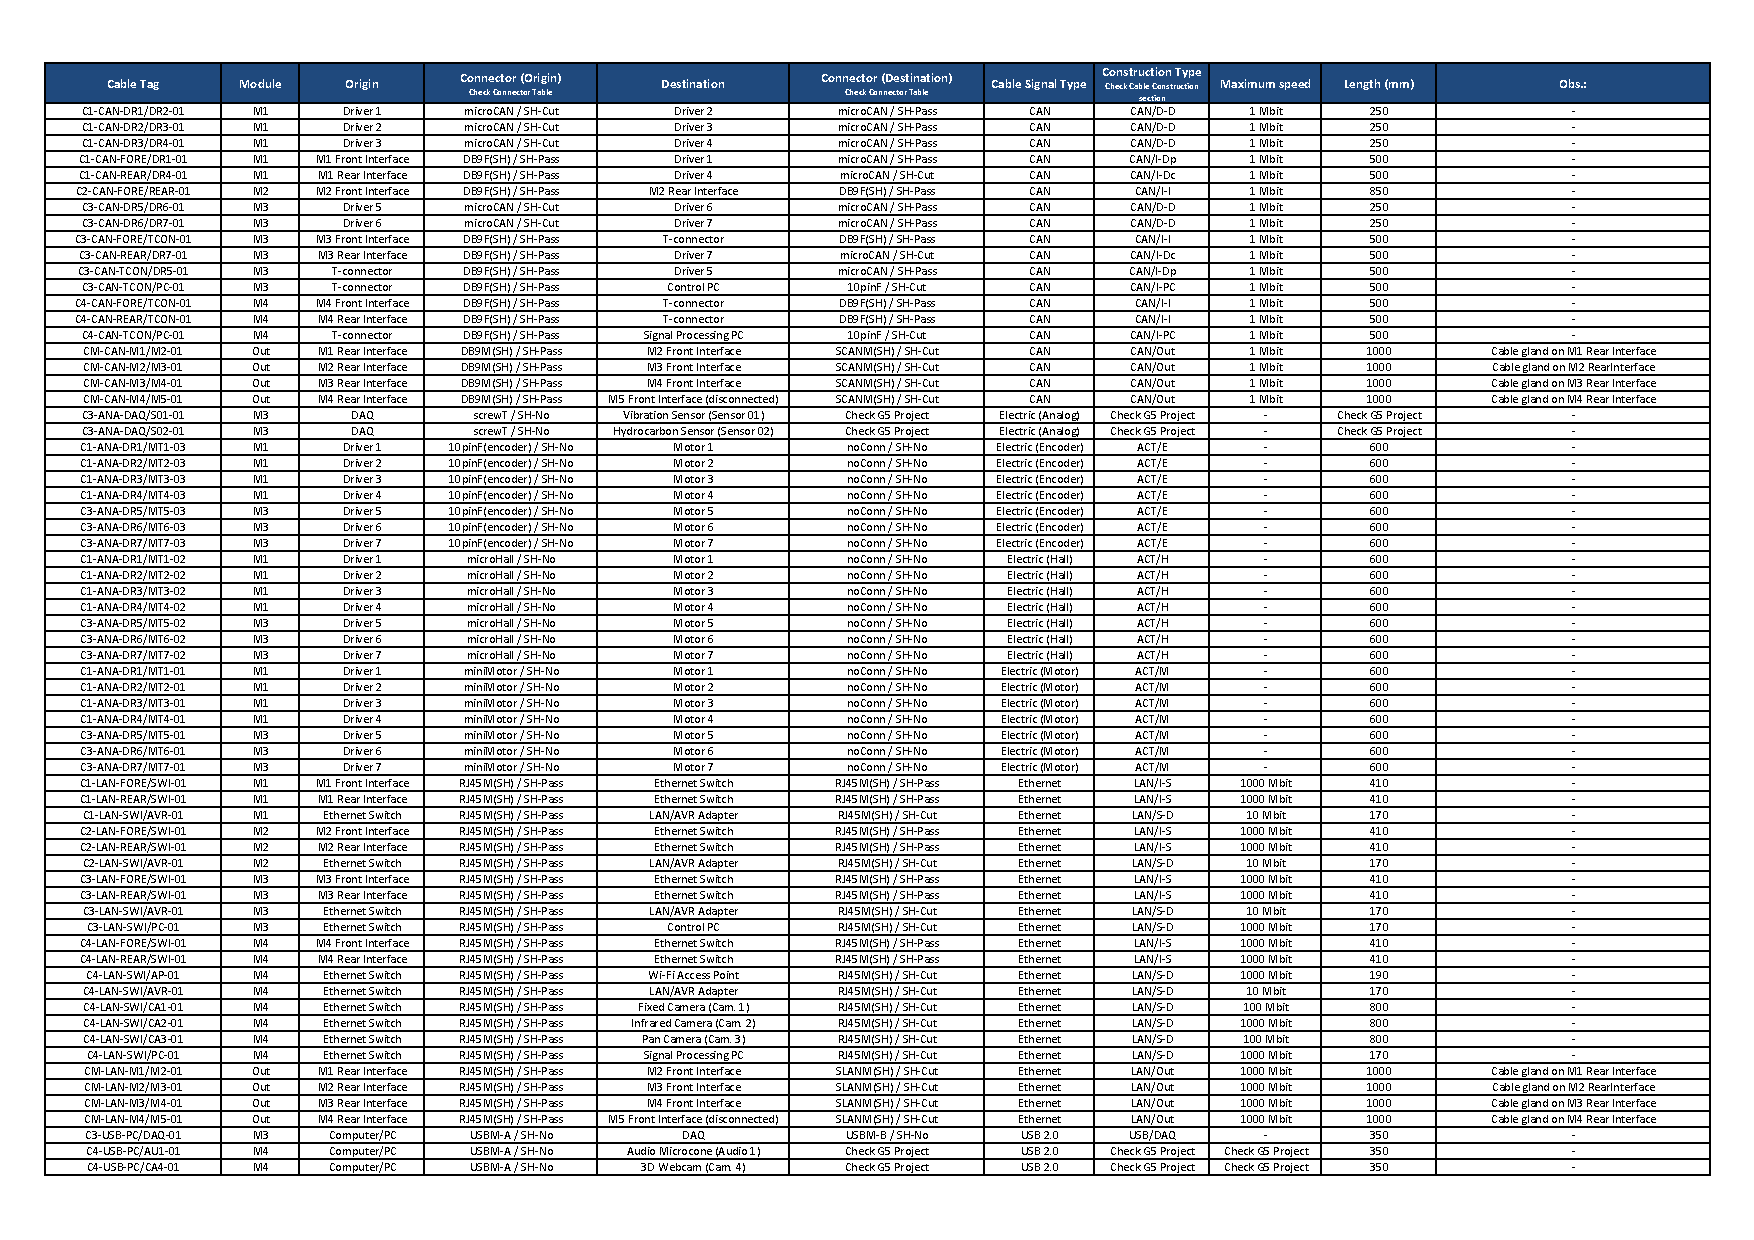
\includegraphics[angle=90,width=1\columnwidth]{figs/body02/FIGCABLELIST.pdf}\\
  \caption[Cable list]{Cable list}
  \label{FIG:CABLELIST}
\end{figure}
\begin{figure}
  \centering
  % Requires \usepackage{graphicx}
  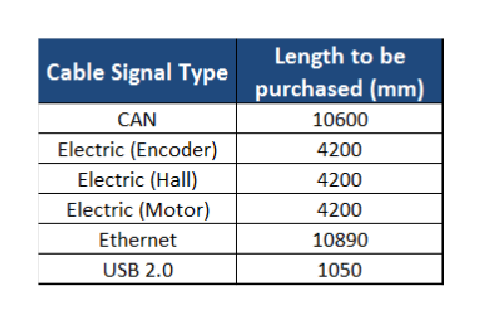
\includegraphics[angle=90,width=1\columnwidth]{figs/body02/FIGCABLETYPELIST.pdf}\\
  \caption[Cable signal type list]{Cable signal type list}
  \label{FIG:CABLETYPELIST}
\end{figure}
\begin{figure}
  \centering
  % Requires \usepackage{graphicx}
  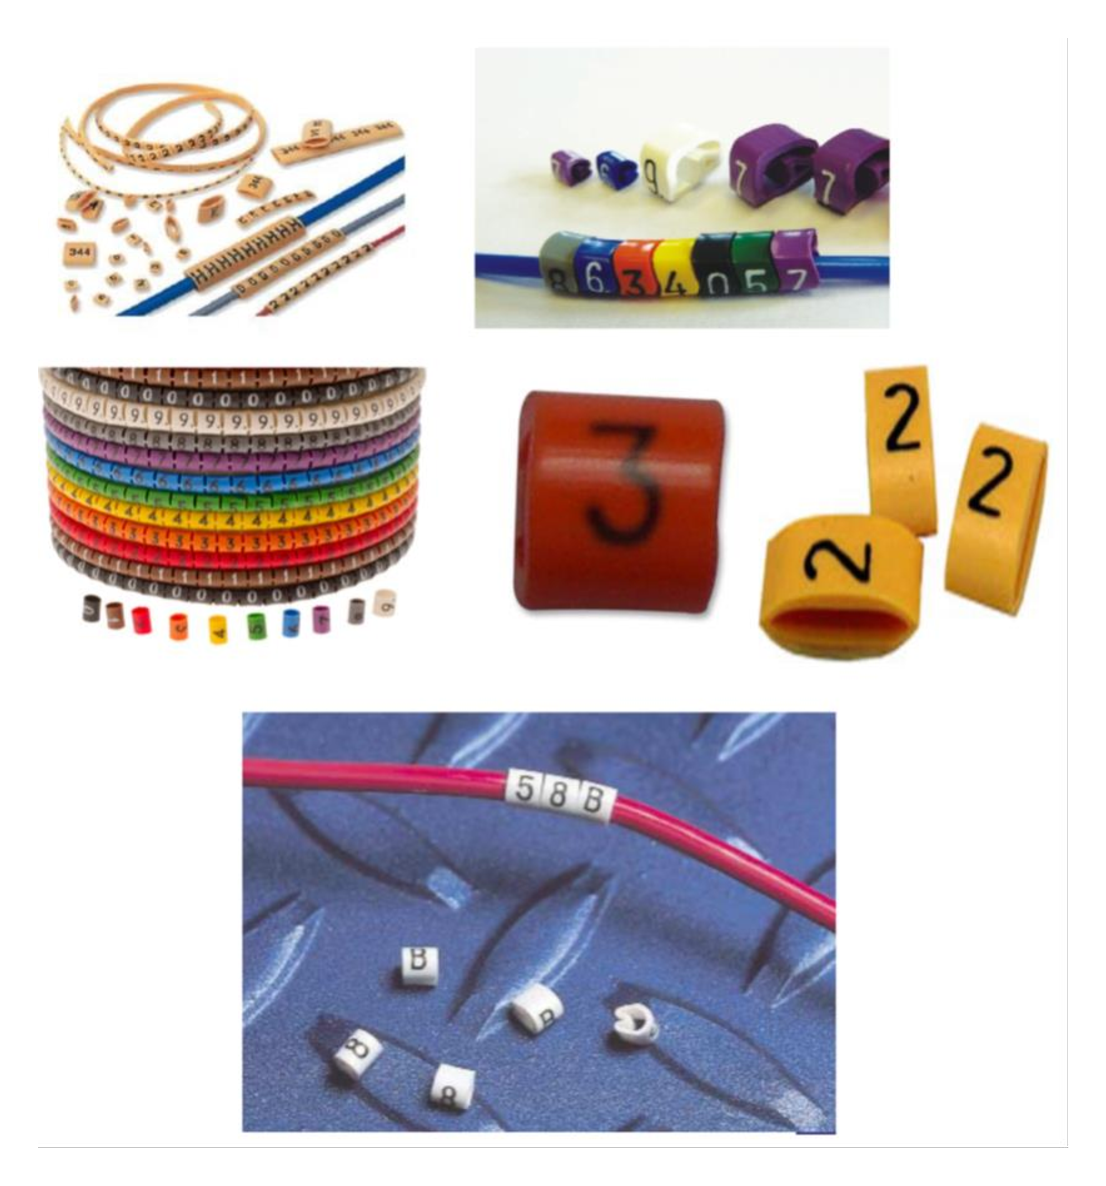
\includegraphics[angle=90,width=1\columnwidth]{figs/body02/FIGOVALGRIP.pdf}\\
  \caption[Cable Mark Type: Ovalgrip]{Cable Mark Type: Ovalgrip}
  \label{FIG:OVALGRIP}
\end{figure}


\subsubsection{Cable signal type: CAN} \label{CABLETYPE:CAN}
\begin{itemize}
  \item Purpose: transmission of CAN
  \item Minimum speed: 1 Mbit
  \item Mean of transmission: 2 twisted pairs
  \item Shielding: 1 shield envelop for all pairs; 1 shield envelop for each pair (optional)
  \item Total length to be purchased: 10600 mm (10.6 m)
  \item Important highlight: Ethernet cable can be used for CAN. For this, use a pair for CAN-High and CAN-Low, a wire from other pair for CAN GND, and the shield envelop.
  \item Commercial models: ESCREVER
\end{itemize}
\subsubsection{Cable signal type: Electric (Encoder)} \label{CABLETYPE:Electric(Encoder)}
\begin{itemize}
  \item Purpose: transmission of Encoder signals from motor encoders to drivers
  \item Mean of transmission: 10 x AWG28, round-jacket, twisted pair flat cable, pitch 1.27 mm
  \item Shielding: No
  \item Total length to be purchased: 4200 mm (4.2 m)
  \item Important highlight: the encoder cable is supplied together with the motor combination (see section~\ref{DEVICE:COMBINATION1}). Instead of purchasing for 4.2 meters of cable for encoder, a better option is ordering 60cm of the encoder cable for each ordered motor combination.
  \item Commercial models: ESCREVER
\end{itemize}
\subsubsection{Cable signal type: Electric (Hall)} \label{CABLETYPE:Electric(Hall)}
\begin{itemize}
  \item Purpose: transmission of Hall sensor signals from motors to drivers
  \item Mean of transmission: 5 x 0.14 mm$^{2}$
  \item Shielding: No
  \item Total length to be purchased: 4200 mm (4.2 m)
  \item Important highlight: the Hall sensor cable is supplied together with the motor combination (see section~\ref{DEVICE:COMBINATION1}). Instead of purchasing for 4.2 meters of cable for Hall sensor, a better option is ordering 60cm of the Hall sensor cable for each ordered motor combination.
  \item Commercial models: ESCREVER
\end{itemize}
\subsubsection{Cable signal type: Electric (Motor)} \label{CABLETYPE:Electric(Motor)}
\begin{itemize}
  \item Purpose: transmission of motor supply and commands from driver
  \item Mean of transmission: 3 x 0.75 mm$^{2}$
  \item Shielding: No
  \item Total length to be purchased: 4200 mm (4.2 m)
  \item Important highlight: the motor supply cable is supplied together with the motor combination (see section~\ref{DEVICE:COMBINATION1}). Instead of purchasing for 4.2 meters of cable for motor supply, a better option is ordering 60cm of the motor supply cable for each ordered motor combination.
  \item Commercial models: ESCREVER
\end{itemize}
\subsubsection{Cable signal type: Ethernet} \label{CABLETYPE:Ethernet}
\begin{itemize}
  \item Purpose: transmission of Ethernet
  \item Minimum speed: 1000 Mbit
  \item Mean of transmission: 4 twisted pairs
  \item Shielding: 1 shield envelop for all pairs; 1 shield envelop for each pair (optional)
  \item Total length to be purchased: 10890 mm (10.89 m)
  \item Commercial models: ESCREVER
\end{itemize}
\subsubsection{Cable signal type: USB 2.0} \label{CABLETYPE:USB20}
\begin{itemize}
  \item Purpose: transmission of USB 2.0
  \item Total length to be purchased: 1050 mm (1.-5 m)
  \item Important highlight: the USB devices generally comes with the specific cable set. However, if needed, this cable can be purchased apart. Generally, 1 meter USB commercial cables can be easily found.
  \item Commercial models: ESCREVER
\end{itemize}
\section{Tools and utilities}
This section presents a list of tools and utilities that must be used for DORIS assembly. In chapter~\ref{CHAPTERASSEMBLY}, some DORIS assembly procedures need the tools that are listed here. This will be indicated as a reference.
\subsection{Tools}
\subsubsection{Heat blower} \label{DEVICE:TOOLTHERMALBLOWER}
\begin{itemize}
  \item Description: The heat blower is the tool used for the application of the heat shrink tubes (see section~\ref{DEVICE:TOOLTHERMALINSULATION}). Generally, heat blowers come as an accessory of soldering stations (see section~\ref{DEVICE:TOOLSOLDERINGSTATION}).
  \item Point the heat blower tip towards the tube (which is already placed over the application area). Continue this procedure until the tube shrunk entirely, hence holding the cable and wires. See figure~\ref{FIG:DEVICEUTILITYHEATSHRINK2} as an illustration.
  \item Examples of models: see figure~\ref{FIG:DEVICEUTILITYHEATSHRINK}
\end{itemize}
\begin{figure}
  \centering
  % Requires \usepackage{graphicx}
  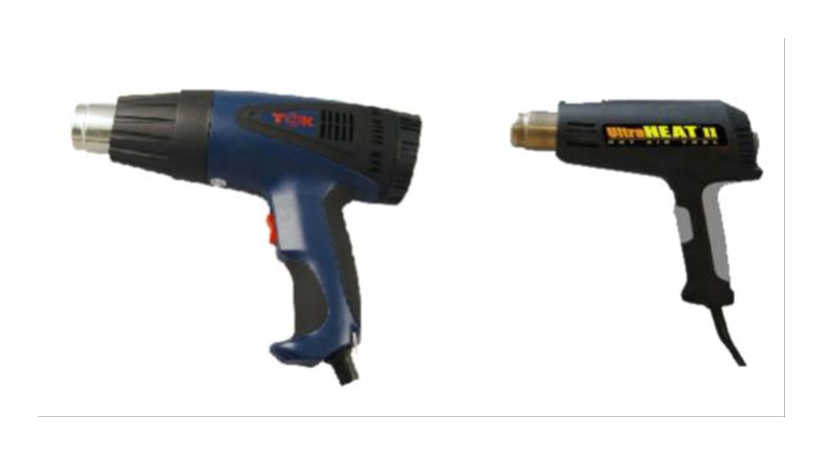
\includegraphics[angle=90,width=1\columnwidth]{figs/body02/FIGDEVICEUTILITYHEATSHRINK.pdf}\\
  \caption[Heat shrink tube for thermal insulation]{Heat shrink tube for thermal insulation}
  \label{FIG:DEVICEUTILITYHEATSHRINK}
\end{figure}
\begin{figure}
  \centering
  % Requires \usepackage{graphicx}
  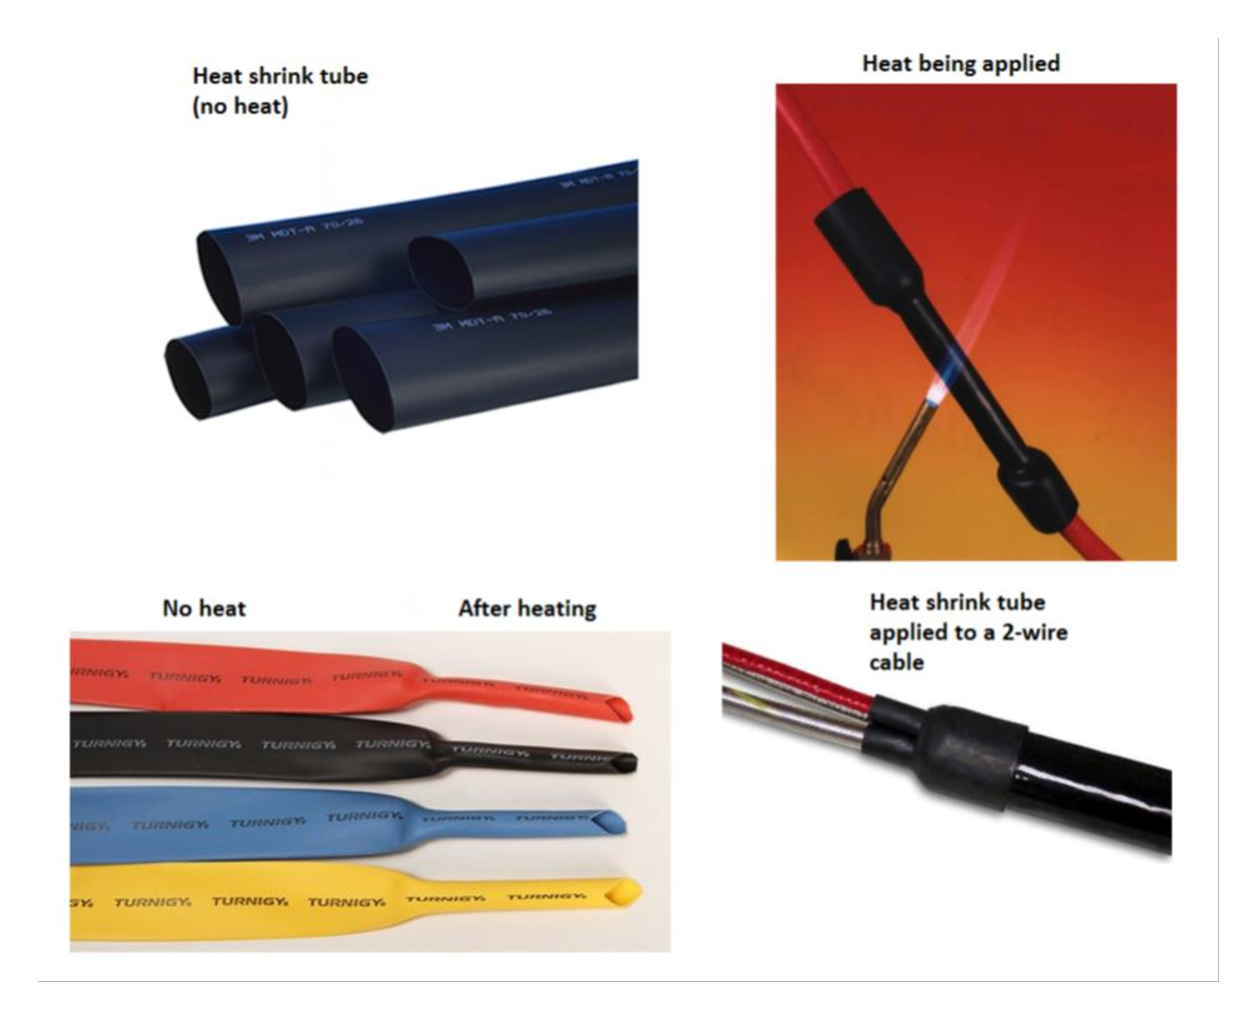
\includegraphics[angle=90,width=1\columnwidth]{figs/body02/FIGDEVICEUTILITYHEATSHRINK2.pdf}\\
  \caption[Heat blower - Application over the cable/wires]{Heat blower - Application over the cable/wires}
  \label{FIG:DEVICEUTILITYHEATSHRINK2}
\end{figure}
\subsubsection{Plier: Cutting plier} \label{DEVICE:TOOLPLIERCUTTING}
\begin{itemize}
  \item Description: This is a cutting plier. It is generally used to cut wires/cables or to strip wire envelops.
  \item Examples of models: see figure~\ref{FIG:DEVICETOOLPLIERCUTTING}
\end{itemize}
\begin{figure}
  \centering
  % Requires \usepackage{graphicx}
  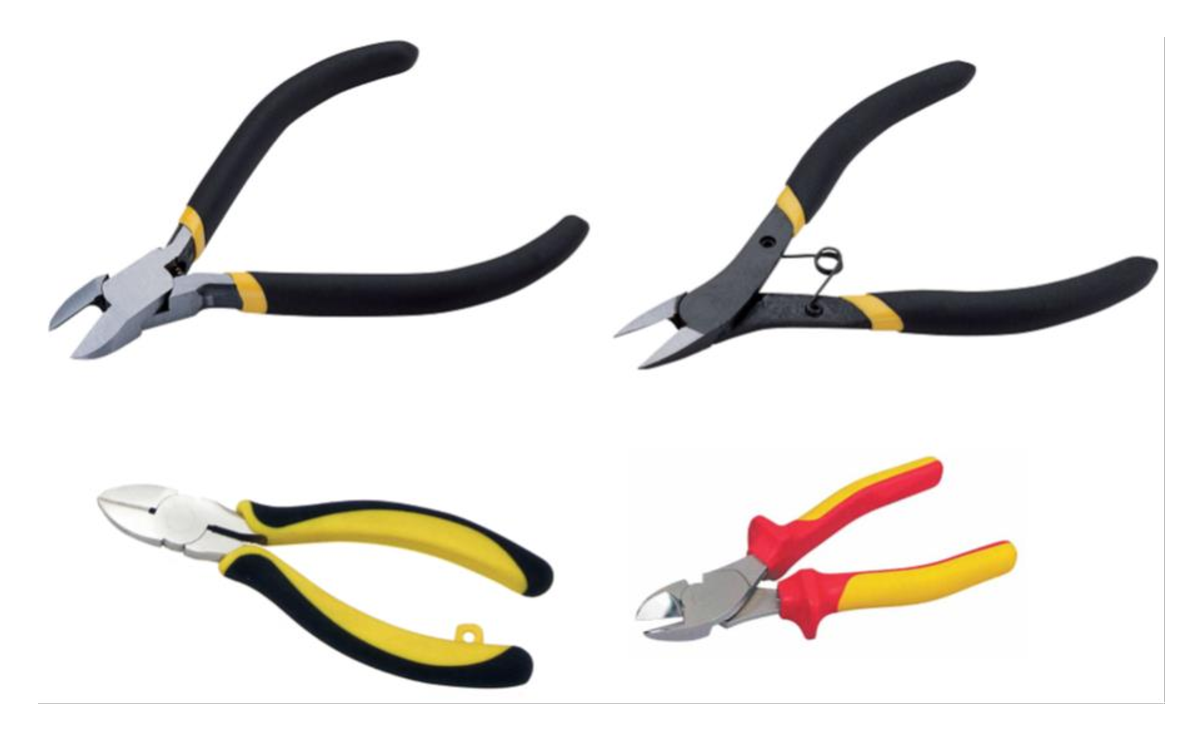
\includegraphics[angle=90,width=1\columnwidth]{figs/body02/FIGDEVICETOOLPLIERCUTTING.pdf}\\
  \caption[Cutting plier examples (out of scale)]{Cutting plier examples (out of scale)}
  \label{FIG:DEVICETOOLPLIERCUTTING}
\end{figure}
\subsubsection{Plier: Long needle-nose plier} \label{DEVICE:TOOLPLIERNEEDLENOSE}
\begin{itemize}
  \item Description: This is a long needle-nose plier. It is generally used to hold wires/cables and strain wire terminals.
  \item Examples of models: see figure~\ref{FIG:DEVICETOOLPLIERNEEDLENOSE}
\end{itemize}
\begin{figure}
  \centering
  % Requires \usepackage{graphicx}
  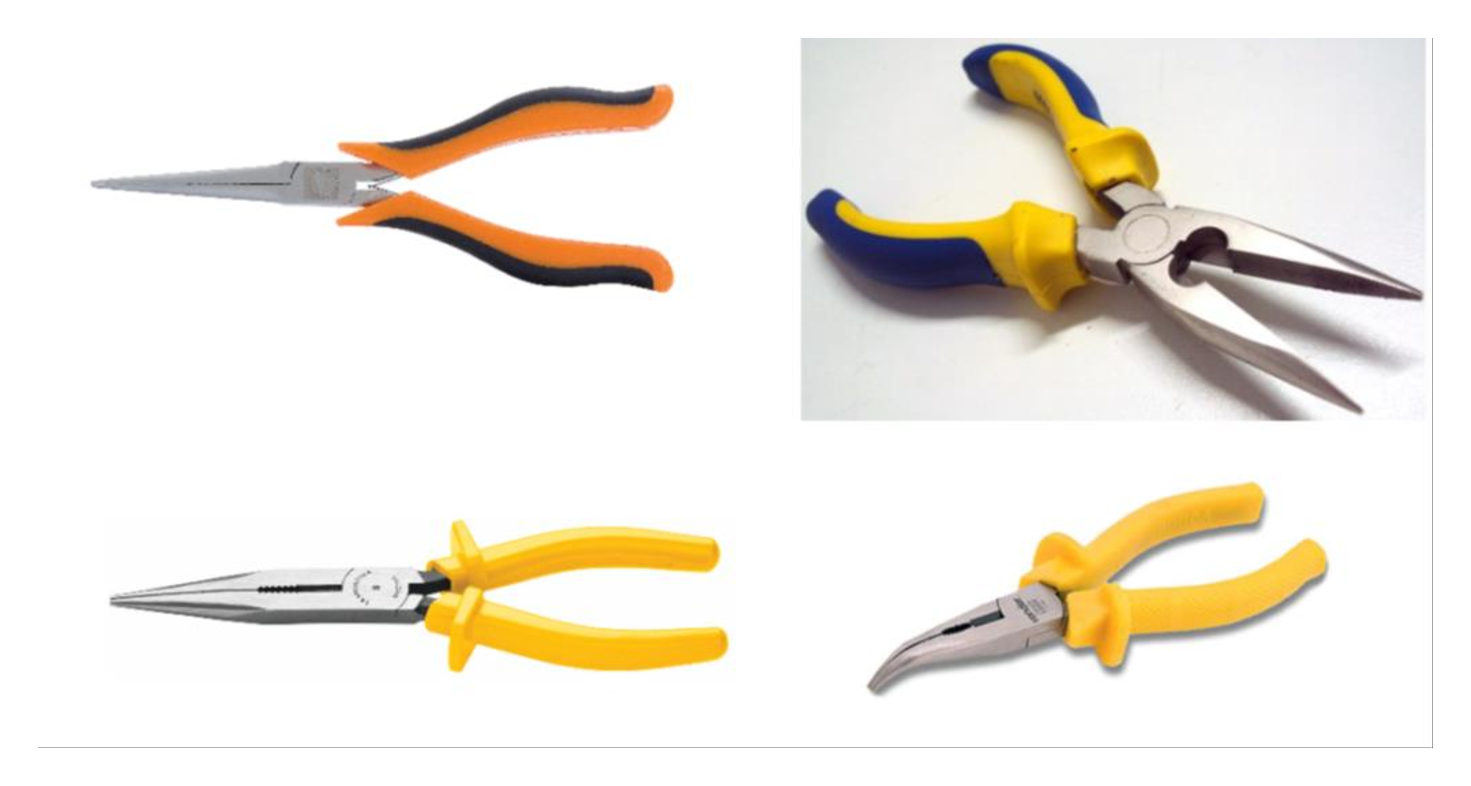
\includegraphics[angle=90,width=1\columnwidth]{figs/body02/FIGDEVICETOOLPLIERNEEDLENOSE.pdf}\\
  \caption[Long needle-nose plier examples (out of scale)]{Long needle-nose plier examples (out of scale)}
  \label{FIG:DEVICETOOLPLIERNEEDLENOSE}
\end{figure}
\subsubsection{Plier: Molex hand crimper for Micro-Fit 3.0 \texttrademark crimp terminals (63819-0000)} \label{DEVICE:TOOLCRIMPERmicro}
\begin{itemize}
\item Name: Molex hand crimper tool for Micro-Fit 3.0\texttrademark crimp terminals, Part Number: 63819-0000
  \item Description: This tool is a special plier for crimping Molex Micro-Fit 3.0\texttrademark female crimp terminals. In DORIS project, it is specially used for crimping the Molex Micro-Fit 3.0\texttrademark female crimp terminals (43030-xxxx family)
  \item Product references (website): \href{http://www.molex.com/molex/products/datasheet.jsp?part=active/0638190000\_APPLICATION\_TOOLIN.xml}{http://www.molex.com/molex/products/datasheet.jsp?part=active/0638190000\_APPLICATION\_TOOLIN.xml}
  \item Commercial option (Website): \href{http://www.digikey.com/product-search/en/tools/crimpers-applicators-presses/1245292?k=63819-0000}{http://www.digikey.com/product-search/en/tools/crimpers-applicators-presses/1245292?k=63819-0000}
  \item Picture: see figure~\ref{FIG:DEVICECRIMPERmicro}
\end{itemize}
\begin{figure}
  \centering
  % Requires \usepackage{graphicx}
  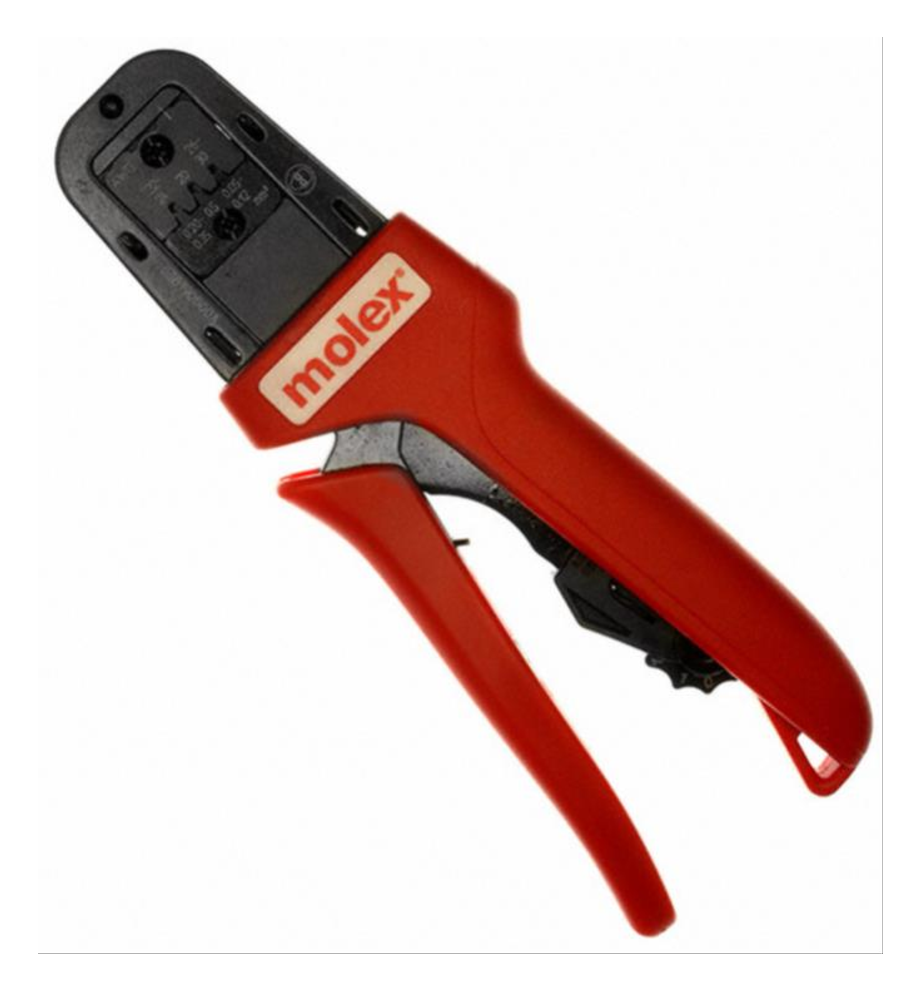
\includegraphics[angle=90,width=1\columnwidth]{figs/body02/FIGDEVICECRIMPERmicro.pdf}\\
  \caption[Plier: Molex hand crimper for Micro-Fit 3.0\texttrademark crimp terminals (63819-0000)]{Plier: Molex hand crimper for Micro-Fit 3.0\texttrademark crimp terminals (63819-0000)}
  \label{FIG:DEVICECRIMPERmicro}
\end{figure}
\subsubsection{Plier: Molex hand crimper for Mini-Fit\textregistered crimp terminals (63819-0900)} \label{DEVICE:TOOLCRIMPERmini}
\begin{itemize}
\item Name: Molex hand crimper tool for Mini-Fit\textregistered crimp terminals, Part Number: 63819-0900
  \item Description: This tool is a special plier for crimping Molex Mini-Fit\textregistered female crimp terminals. In DORIS project, it is specially used for crimping the Molex Mini-Fit\textregistered female crimp terminals (44476-xxxx family)
  \item Product references (website): \href{http://www.molex.com/molex/products/datasheet.jsp?part=active/0638190900\_APPLICATION\_TOOLIN.xml}{http://www.molex.com/molex/products/datasheet.jsp?part=active/0638190900\_APPLICATION\_TOOLIN.xml}
  \item Commercial option (Website): \href{http://www.digikey.com/product-search/en/tools/crimpers-applicators-presses/1245292?k=63819-0900}{http://www.digikey.com/product-search/en/tools/crimpers-applicators-presses/1245292?k=63819-0900}
  \item Picture: see figure~\ref{FIG:DEVICECRIMPERmini}
\end{itemize}
\begin{figure}
  \centering
  % Requires \usepackage{graphicx}
  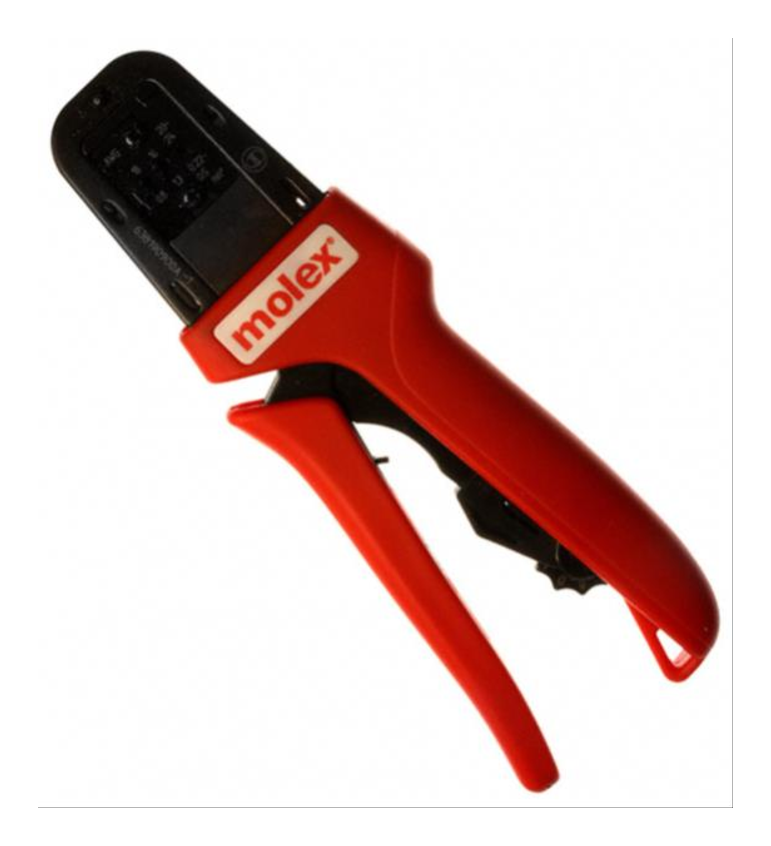
\includegraphics[angle=90,width=1\columnwidth]{figs/body02/FIGDEVICECRIMPERmini.pdf}\\
  \caption[Plier: Molex hand crimper for Mini-Fit\textregistered crimp terminals (63819-0900)]{Plier: Molex hand crimper for Mini-Fit\textregistered crimp terminals (63819-0900)}
  \label{FIG:DEVICECRIMPERmini}
\end{figure}
\subsubsection{Soldering station} \label{DEVICE:TOOLSOLDERINGSTATION}
\begin{itemize}
  \item Description: The soldering station is the tool used for general welding. the application of the heat shrink tubes (see section~\ref{DEVICE:TOOLTHERMALINSULATION}).
  \item Features: Generally, the soldering station comes with: a soldering iron, support for soldering iron, heat blower, power supply.
  \item Example of model: see figure~\ref{FIG:DEVICESOLDERINGSTATION}
\end{itemize}
\begin{figure}
  \centering
  % Requires \usepackage{graphicx}
  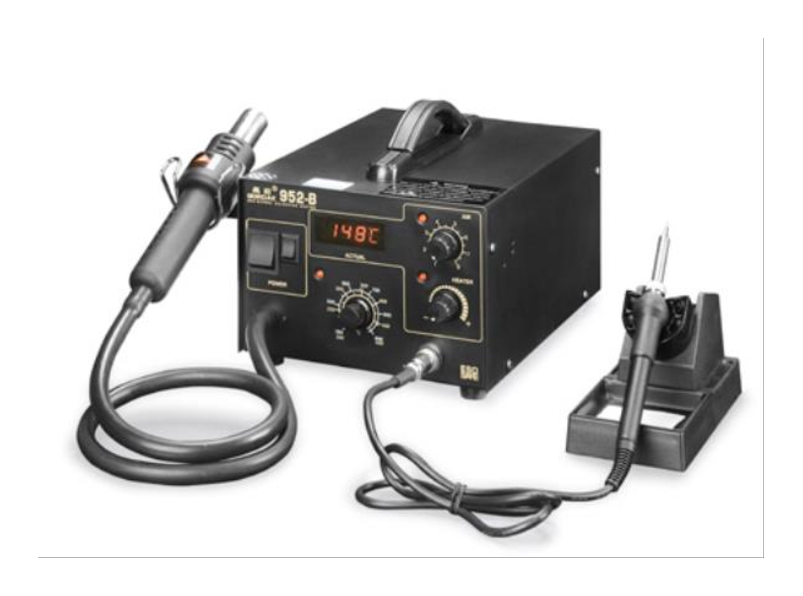
\includegraphics[angle=90,width=1\columnwidth]{figs/body02/FIGDEVICESOLDERINGSTATION.pdf}\\
  \caption[Soldering station]{Soldering station}
  \label{FIG:DEVICESOLDERINGSTATION}
\end{figure}
\subsection{Utilities}
\subsubsection{Heat shrink tube for thermal insulation} \label{DEVICE:TOOLTHERMALINSULATION}
\begin{itemize}
  \item Description: This tube is applied on parts of the cable that require isolation, such as the sections near connectors or striped wire/cable envelops. Commercial models with different diameters can be found. Each tube diameter is suitable for a specific wire/cable gauge on which the application will be done.
  \item Application procedure: The application of a heat shrink on a cable requires a heat blower(see section~\ref{DEVICE:TOOLTHERMALBLOWER}). First, select the right tube diameter and length (generally, 2cm length are reasonable). Afterwards, place this tube piece over the application area, covering the whole cable and internal wires. Then, point the heat blower tip towards the tube. Continue this procedure until the tube shrunk entirely, hence holding the cable and wires. See figure~\ref{FIG:DEVICEUTILITYHEATSHRINK2} as an illustration.
  \item Examples of models: see figure~\ref{FIG:DEVICEUTILITYHEATSHRINK1}
\end{itemize}
\begin{figure}
  \centering
  % Requires \usepackage{graphicx}
  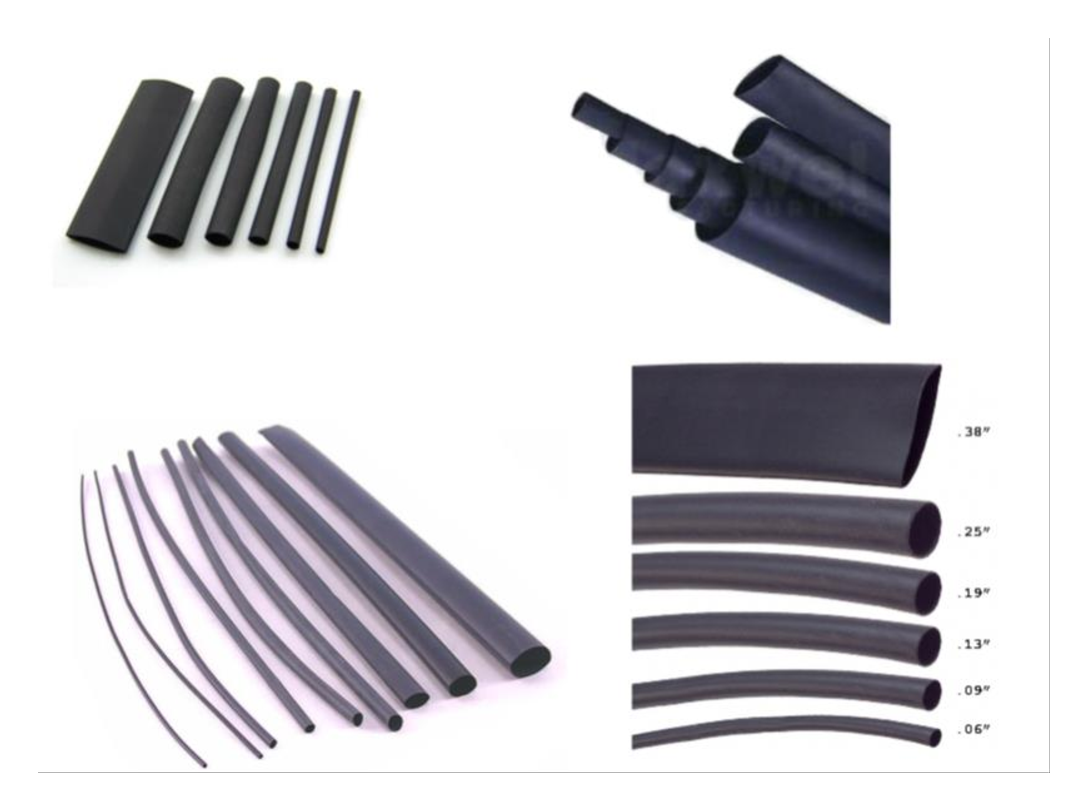
\includegraphics[angle=90,width=1\columnwidth]{figs/body02/FIGDEVICEUTILITYHEATSHRINK1.pdf}\\
  \caption[Heat shrink tube for thermal insulation]{Heat shrink tube for thermal insulation}
  \label{FIG:DEVICEUTILITYHEATSHRINK1}
\end{figure}
\begin{figure}
  \centering
  % Requires \usepackage{graphicx}
  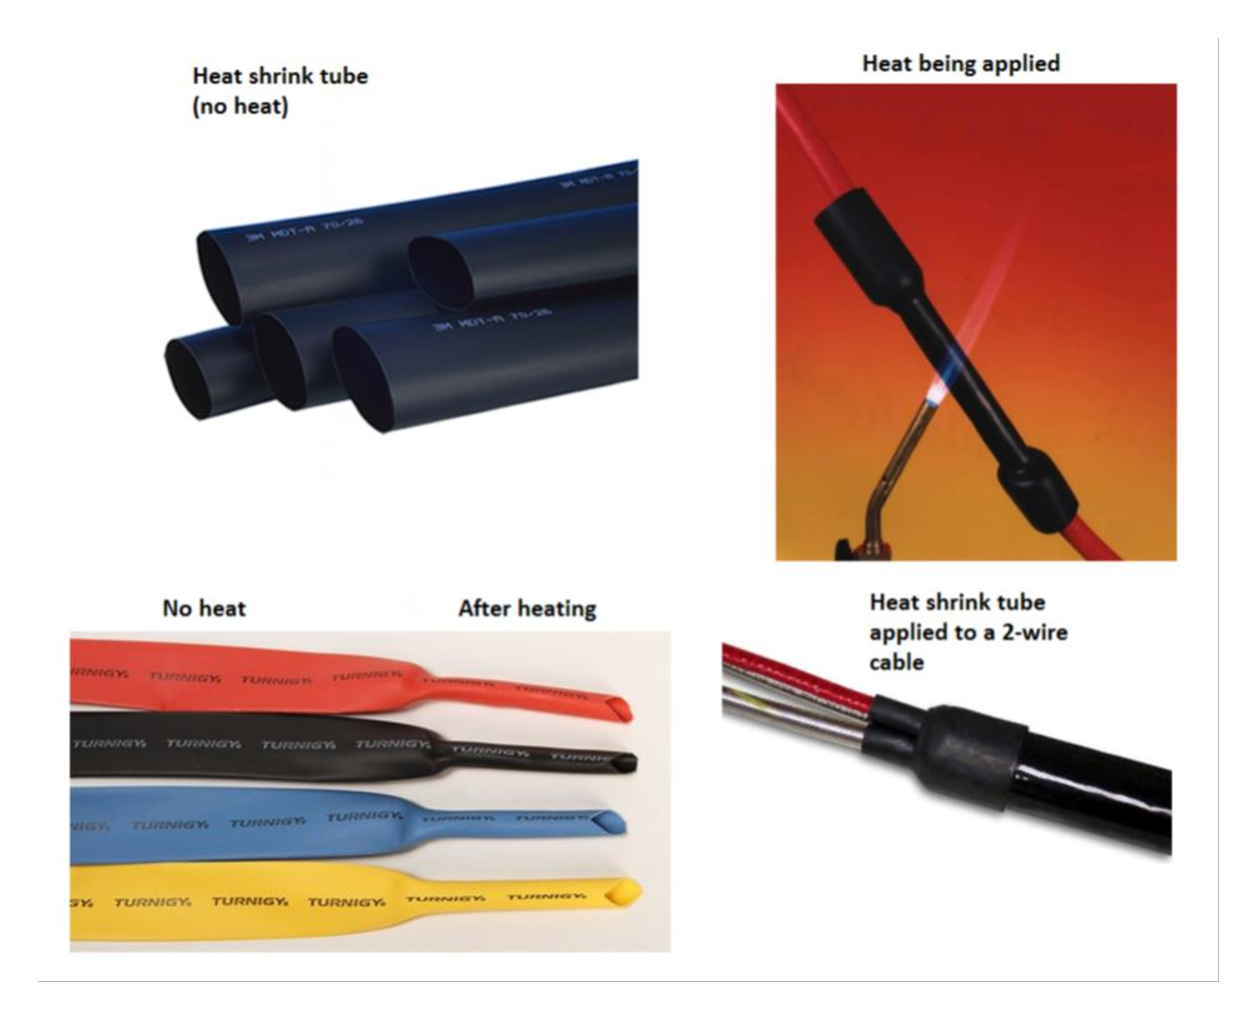
\includegraphics[angle=90,width=1\columnwidth]{figs/body02/FIGDEVICEUTILITYHEATSHRINK2.pdf}\\
  \caption[Heat shrink tube for thermal insulation - Application over the cable/wires]{Heat shrink tube for thermal insulation - Application over the cable/wires}
  \label{FIG:DEVICEUTILITYHEATSHRINK2}
\end{figure}
\subsubsection{microCrimp: Molex Micro-Fit 3.0\texttrademark female crimp terminals (43030-xxxx)} \label{DEVICE:microCrimp}
\begin{itemize}
  \item Acronym for cable/connector lists: microCrimp
  \item Name: Molex Micro-Fit 3.0\texttrademark female crimp terminals, Part Number: 43030-xxxx (there are many metal and color options). In this section, the part number 43030-0002 is being used as an example.
  \item Description: This crimp terminal is used to crimp the wire ends which are fitted in Molex Micro-Fit 3.0\texttrademark connectors 43025-xxxx family (sections~\ref{DEVICE:microCAN} and~\ref{DEVICE:microHall}).
  \item Model references (Website): \href{http://www.molex.com/molex/products/datasheet.jsp?part=active/0430300002\_CRIMP\_TERMINALS.xml}{http://www.molex.com/molex/products/datasheet.jsp?part=active/0430300002\_CRIMP\_TERMINALS.xml}
  \item Picture: see figure~\ref{FIG:DEVICEmicroCrimp}
  \item Commercial option (Website): \href{http://www.digikey.com/product-detail/en/0430300002/WM1125TR-ND/467797}{http://www.digikey.com/product-detail/en/0430300002/WM1125TR-ND/467797}
\end{itemize}
\begin{figure}
  \centering
  % Requires \usepackage{graphicx}
  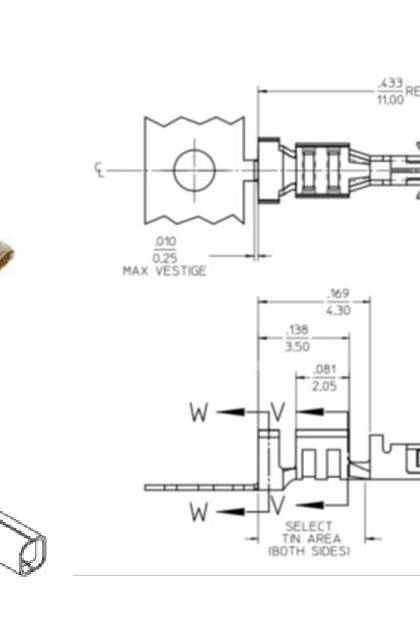
\includegraphics[angle=90,width=1\columnwidth]{figs/body02/FIGDEVICEmicroCrimp.pdf}\\
  \caption[microCrimp: Molex Micro-Fit 3.0\texttrademark female crimp terminals (43030-xxxx)]{microCrimp: Molex Micro-Fit 3.0\texttrademark female crimp terminals (43030-xxxx)}
  \label{FIG:DEVICEmicroCrimp}
\end{figure}
\subsubsection{miniCrimp: Molex Mini-Fit\textregistered Jr. female crimp terminals (44476-xxxx)} \label{DEVICE:miniCrimp}
\begin{itemize}
  \item Acronym for cable/connector lists: miniCrimp
  \item Name: Molex Mini-Fit\textregistered Jr. female crimp terminals, Part Number: 44476-xxxx (there are many metal and color options). In this section, the part number 44476-1112 is being used as an example.
  \item Description: This crimp terminal is used to crimp the wire ends which are fitted in Molex Mini-Fit\textregistered connectors 44476-xxxx family (sections~\ref{DEVICE:miniMotor} and~\ref{DEVICE:miniPower}).
  \item Model references (Website): \href{http://www.molex.com/molex/products/datasheet.jsp?part=active/0444761112\_CRIMP\_TERMINALS.xml}{http://www.molex.com/molex/products/datasheet.jsp?part=active/0444761112\_CRIMP\_TERMINALS.xml}
  \item Picture: see figure~\ref{FIG:DEVICEminiCrimp}
  \item Commercial option (Website): \href{http://www.digikey.com/product-detail/en/0444761112/WM1914-ND/283456}{http://www.digikey.com/product-detail/en/0444761112/WM1914-ND/283456}
\end{itemize}
\begin{figure}
  \centering
  % Requires \usepackage{graphicx}
  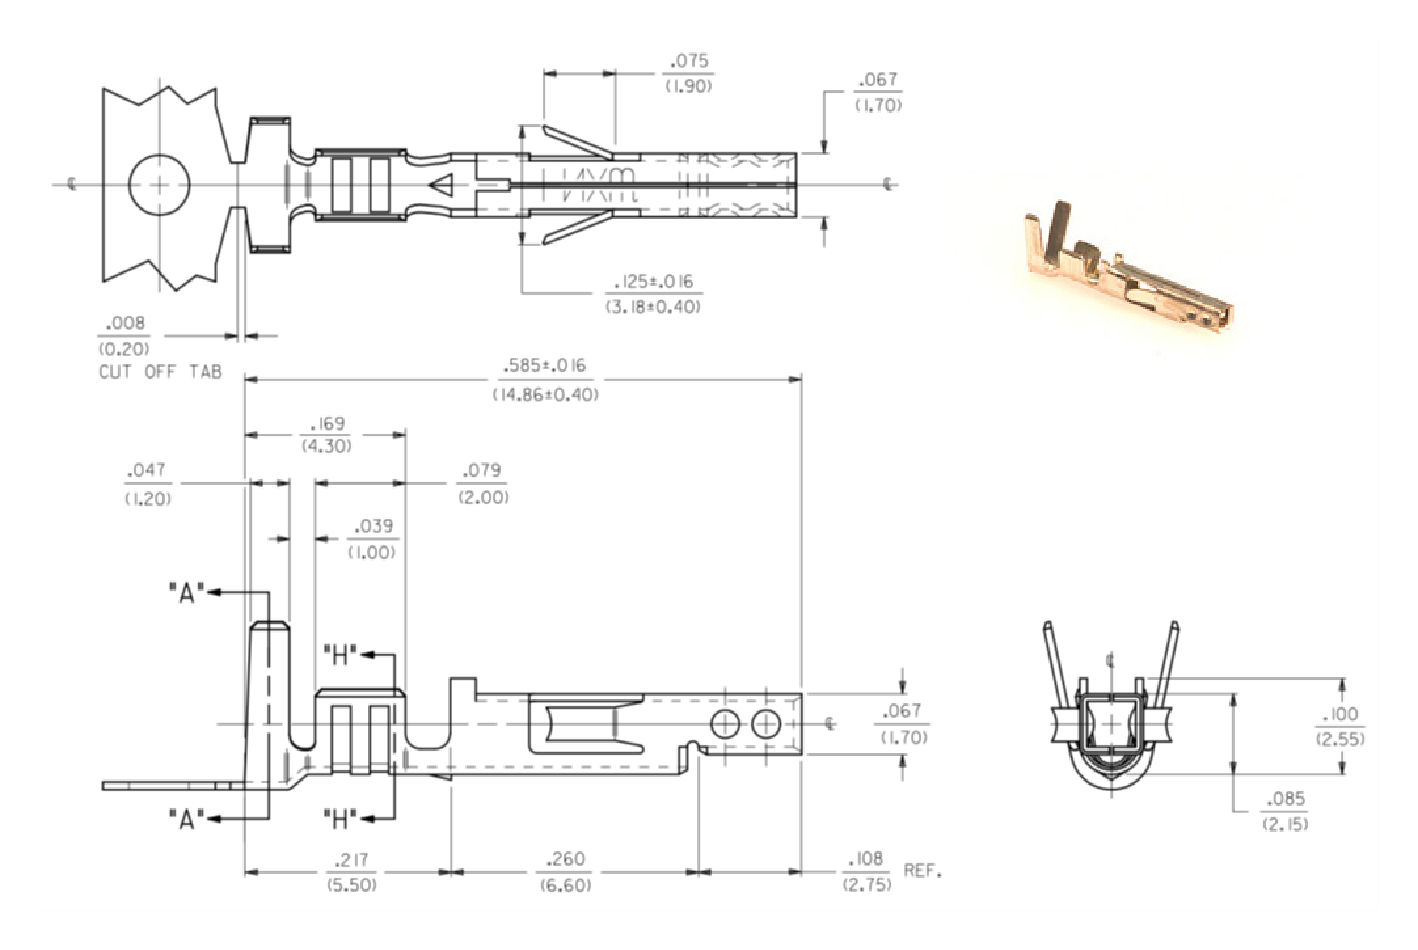
\includegraphics[angle=90,width=1\columnwidth]{figs/body02/FIGDEVICEminiCrimp.pdf}\\
  \caption[miniCrimp: Molex Mini-Fit\textregistered Jr. female crimp terminals (44476-xxxx)]{miniCrimp: Molex Mini-Fit\textregistered Jr. female crimp terminals (44476-xxxx)}
  \label{FIG:DEVICEminiCrimp}
\end{figure} 